% =====================================================================
%  companion_categorical_v8.tex -- standalone theory paper.
%  ---------------------------------------------------------------
%  Role:       full development of the categorical and
%              homotopy-theoretic framework for viability-
%              weighted curvature: the SAVGS object, the 2-category
%              StCon(B) of stratified connections with the gluing
%              theorem and the piecewise-holonomy formula, the
%              Fisher-minimal transport law on constant-active-set
%              strata, the Bregman--Noether correspondence, the
%              seven-optic composition theorem with per-optic
%              Lipschitz constants and the Banach contraction, the
%              filtered-colimit construction of RAF sets, and the
%              HoTT/infty-categorical extension.
%  Relation:   the application paper (journal_manuscript_v10.tex)
%              states the load-bearing definitions of this
%              framework in brief adapted form and cites this
%              development for the constructions and proofs; this
%              paper cites the application paper where the empirical
%              line is concerned. Each paper is self-contained for
%              its own claims.
%  Gemini-alignment round (v7 -> v8): narrative harm-in-sequence
%              abstract opening (net word-neutral; < 265 cap kept),
%              the concrete closed-cycle example in the Introduction,
%              the intuitive gloss at the viability-weighted curvature
%              definition, an in-words gloss at the optic category
%              definition, the stabilization question at the head of
%              the Lipschitz section, the application-bridge numbers
%              in the Introduction, and a compact Conclusion section.
%              Every numerical claim is unchanged from v7.
%  Provenance: machine-verification scripts and artifacts are
%              committed in the repository (Data Availability).
%  Proof status is labeled per theorem: complete proofs; proofs
%              that reduce to cited descent/coherence theory
%              (marked); proof sketches (marked); machine-verified
%              statements with committed artifacts. Conjectures stay
%              conjectures.
% =====================================================================
\documentclass[11pt,a4paper]{article}

\usepackage{amsmath,amssymb,amsthm}
\usepackage{mathtools}
\usepackage{mathrsfs}
\usepackage[margin=2.4cm]{geometry}
\usepackage{microtype}
\usepackage{booktabs}
\usepackage{tabularx}
\usepackage{enumitem}
\usepackage{xcolor}
\usepackage{graphicx}
\graphicspath{{./}{../download/}}
\usepackage[colorlinks=true,linkcolor=blue!55!black,citecolor=blue!45!black,urlcolor=blue!55!black,bookmarks=true,bookmarksnumbered=true,unicode=true]{hyperref}
\usepackage[round]{natbib}

% Theorem environments
\theoremstyle{plain}
\newtheorem{theorem}{Theorem}[section]
\newtheorem{proposition}[theorem]{Proposition}
\newtheorem{lemma}[theorem]{Lemma}
\newtheorem{corollary}[theorem]{Corollary}
\theoremstyle{definition}
\newtheorem{definition}[theorem]{Definition}
\newtheorem{construction}[theorem]{Construction}
\newtheorem{assumption}[theorem]{Assumption}
\newtheorem{conjecture}[theorem]{Conjecture}
\theoremstyle{remark}
\newtheorem{remark}[theorem]{Remark}

% Macros
\newcommand{\kk}{\kappa_{\!V}}
\newcommand{\HH}{\mathcal{H}}
\newcommand{\OO}{\mathcal{O}}
\newcommand{\CC}{\mathcal{C}}
\newcommand{\RR}{\mathbb{R}}
\newcommand{\PP}{\mathbb{P}}
\newcommand{\SO}{\mathrm{SO}}
\newcommand{\CO}{\mathrm{CO}}
\newcommand{\so}{\mathfrak{so}}
\newcommand{\Stab}{\mathrm{Stab}}
\newcommand{\End}{\mathrm{End}}
\newcommand{\Optic}{\mathbf{Optic}}
\newcommand{\RAF}{\mathrm{RAF}}
\newcommand{\colim}{\operatorname{colim}}
\newcommand{\id}{\mathrm{id}}
\newcommand{\sgn}{\operatorname{sgn}}
\newcommand{\Frob}{\!\operatorname{}\!\mathopen{}\Vert\cdot\mathclose{}\Vert_{\!F}}
\newcommand{\normF}[1]{\mathopen{}\Vert#1\mathclose{}\Vert_{\!F}}
\newcommand{\distD}{\mathrm{dist}_{D}}
\newcommand{\SAVGS}{\mathrm{SAVGS}}
\DeclareMathOperator{\Lip}{Lip}
\newcommand{\kmu}{\kappa^{\mu}}

\hypersetup{
 pdftitle={Stratified Connections, Optic Composition, and the
           Homotopy Fixed-Point Extension: A Categorical Framework
           for Viability-Weighted Curvature},
 pdfauthor={Amin Abaee},
 pdfsubject={categorical framework for viability-weighted curvature:
             stratified connections, optic composition, homotopy
             type theory},
 pdfkeywords={optic category, stratified connection, 2-category,
              filtered colimit, homotopy type theory,
              applied category theory}}

\widowpenalty=10000
\clubpenalty=10000
\emergencystretch=3em
\hbadness=2500
\vbadness=2500

\begin{document}

\begin{center}
  \vspace*{0.4em}
  {\large\bfseries Stratified Connections, Optic Composition, and the
   Homotopy Fixed-Point Extension:\par
   A Categorical Framework for Viability-Weighted Curvature\par}
  \vspace{0.8em}
  {\normalsize Amin Abaee\par}
  \vspace{0.3em}
  {\small\itshape Independent Researcher, Tehran, Iran\par}
  {\small\itshape amin\_abaee@ut.ac.ir\ \textbullet\ ORCID 0000-0002-0019-1842\par}
  \vspace{0.2em}
  {\small\itshape Preprint, September 2026\par}
  \vspace{0.6em}
  \rule{0.7\textwidth}{0.4pt}
\end{center}

\vspace{0.6em}
\begin{center}
\begin{minipage}{0.92\textwidth}
\small
\textbf{Abstract.} An adaptive system must stay viable while its
environment changes; its policy is optimal subject to active
constraints, and a closed sequence of manageable changes can
accumulate into a threat. We develop the categorical and
homotopy-theoretic framework for viability-weighted curvature: the
geometric object measuring this accumulation through the policy
holonomy.
(i)~The SAVGS object assembles control base, Fisher--Rao
policy bundle, viability margin, maintenance graph, and a
$2$-categorical boundary span into one stratified bundle.
(ii)~The $2$-category $\mathbf{StCon}(B)$ of stratified
$G_C$-connections carries a lax-functorial gluing theorem, a
piecewise-holonomy formula, and the small-loop expansion for loops
crossing a constraint-switching wall transversally in
\emph{pairs}; on constant-active-set strata the connection is the
Fisher-minimal transport law (KKT projection), and the small-loop
viability--holonomy theorem bounds endpoint erosion of a viability
margin by the viability-weighted curvature, its worst-case
positive-part contraction with active survival covectors.
(iii)~A single composition theorem types the seven domain bridges
as optics, establishing a per-optic Lipschitz bound and a Banach
contraction of the Krasnoselskii--Mann-averaged update for its
instantiation; the projected CPTP contraction
settles the Zeno self-reference.
(iv)~The filtered-colimit construction of RAF sets is proved at Set
level with an adapter-level optic statement, verified at scale;
the $\infty$-categorical extension is developed in homotopy type
theory, proof-sketch status marked. The validation battery is
robust across six axes: carbon, oxygen, nitrogen,
phosphate, and iron supply plus non-medium maintenance stress
leave labels invariant, re-stratifying only at
regime switches; the association is invariant under canonical
flux selection, the declared tie-break closing its near-degeneracy
boundary. The application paper
develops the atomic curvature measure and its genome-scale
validation.
\par
\vspace{0.5em}

\noindent\textbf{Keywords:} optic category; stratified connection;
2-category; filtered colimit; homotopy type theory;
applied category theory\\[0.3em]
\noindent\textbf{AMS 2020 Subject Classification:} 18D05; 18N99;
92B05\par
\end{minipage}
\end{center}

\tableofcontents
\newpage

% =====================================================================
\section{Introduction}\label{sec:role}

\paragraph{The problem.}
An adaptive system that must remain viable while its environment
changes is governed, at each instant, by a policy that is optimal
subject to active constraints. A \emph{policy} is the optimizer's
chosen response at each state; a \emph{connection} is the rule for
comparing policies at nearby states; and its \emph{holonomy} is the
drift accumulated around a closed loop of changes --- the geometric
signature of non-commutativity. In concrete terms: a system can
survive a change in temperature, and separately survive a change in
nutrient supply; applied as a closed cycle --- temperature, then
nutrients, then reverse temperature, then reverse nutrients --- the
same two changes can still return the system to its starting
environment with its internal reserves degraded. The order matters,
not only the magnitudes: adjustments governed by active constraints
need not commute. Classical viability theory \citep{aubin2011} supplies
set-valued dynamics and tangential conditions, but no
\emph{geometric} object that measures how a non-commuting sequence
of individually manageable changes accumulates into a viability
threat. The obstruction is structural: at a constraint-switching
boundary the active set changes, horizontal subspaces jump, the
connection $1$-form ceases to be defined, and the standard holonomy
integral fails exactly where the question is most interesting. This
paper constructs the missing object categorically: a stratified
connection with a boundary gluing law, a viability-weighted
curvature that contracts the curvature $2$-form with survival
covectors, and a compositional semantics (optics --- a map paired
with its feedback channel) under which
heterogeneous domain bridges compose into one typed endomorphism
whose fixed point is well posed and, for an explicit
instantiation, contractive.

\paragraph{Contributions.}
\begin{enumerate}[leftmargin=*,itemsep=2pt]
\item The \emph{SAVGS object}
(Definition~\ref{def:savgs}): control base, policy bundle with
Fisher--Rao geometry, viability margin, maintenance graph, and a
$2$-categorical boundary span, assembled into one stratified
$G_C$-reduced bundle.
\item The $2$-category $\mathbf{StCon}(B)$ of stratified
$G_C$-connections (Definition~\ref{def:stcon}), the
$2$-categorical gluing theorem (Theorem~\ref{thm:2cat-gluing}), and
the piecewise holonomy formula
(Theorem~\ref{thm:stratified-holonomy}), with the small-loop
expansion stated for closed loops crossing a switching wall
transversally in pairs and the boundary-reset contribution at its
true order, in agreement with the machine-verified numerics in
five loop geometries and three structure-group regimes.
\item The \emph{Fisher-minimal transport law} on
constant-active-set strata in closed KKT form
(Proposition~\ref{prop:kkt}) and the \emph{small-loop
viability--holonomy theorem} (Theorem~\ref{thm:smallloop}): endpoint
erosion of a viability margin is bounded, to leading order, by the
viability-weighted curvature
(Definition~\ref{def:kv}).
\item The Bregman--Hessian Noether correspondence
(Proposition~\ref{prop:noether}) with its falsifiable precondition
check, giving the gauge-covariance statement for the curvature.
\item The \emph{single composition theorem}
(Theorem~\ref{thm:composition}): seven domain bridges typed as
optics, the realized update on a complete metric state space
(Definition~\ref{def:realization}), per-optic analytic Lipschitz
constants (Lemma~\ref{lem:lip-per-optic}), the Banach contraction
of the Krasnoselskii--Mann-averaged update for the chosen seven-map
instantiation (Theorem~\ref{thm:unconditional-banach}), and the
projected CPTP channel contraction
(Theorem~\ref{thm:zeno-contraction}) settling the Zeno
self-reference resolution.
\item The filtered-colimit construction of RAF sets, proved at the
Set level with the adapter-level optic statement
(Theorem~\ref{thm:filtered-colimits-optic}) and verified at scale
(Proposition~\ref{prop:invlim-extended}).
\item The $\infty$-categorical extension via homotopy type theory
(Theorem~\ref{thm:hott-composition},
Corollary~\ref{cor:hott-fixedpoint}), with proof-sketch status
explicitly marked (Remark~\ref{rem:proof-status-hott}), and the
three-phase autopoiesis closure test built on it
(Definition~\ref{def:autopoiesis-phase3}).
\end{enumerate}

\paragraph{Relation to the application paper.}
An application of this framework to metabolic flux rerouting appears
in a separate manuscript \citep{zai2026measure}: there the
viability-weighted-curvature idea is realized measure-theoretically
as an atomic curvature measure on the active-set complex of
parametric flux balance analysis, a gene-level sensitivity metric
$\kappa^{\mu}$ is derived from it, and the metric is validated at
genome scale against carbon-depletion transcriptional response
($r = +0.395$, $n = 424$ genes), with an explicit protein-layer null
($r = -0.083$ on matched quantitative proteomics, $n = 366$) and
selection-rule robustness checks. The application paper states the load-bearing definitions
of the present framework in brief, adapted form and cites this
paper for the constructions, machine verifications, and proofs at
the status marked per result --- complete proofs for the gluing
formula, the Fisher-minimal transport law, the composition and
contraction layers, and the terminal-coalgebra theorem;
machine-verified statements for the numerics; citation-level
reduction for the stratified descent; proof-sketch status, marked
as such, for the homotopy-type-theoretic extension. The present
paper develops the full categorical machinery and cites the
application paper where the empirical line is concerned. The division of labor is
deliberate: the empirical claims of the application paper are
statistical, the categorical claims of this
paper are mathematical, and neither paper depends on the other's
claims.

\paragraph{Status conventions.}
Theorem-level claims are labeled by proof status throughout:
complete proofs; proofs that reduce to cited descent or coherence
theory (marked in remarks); proof sketches (marked); and
machine-verified statements, whose scripts and artifacts are
committed in the project repository and regenerated by them. Open
problems are collected in Section~\ref{sec:future}.

\section{Preliminaries}\label{sec:prelim}
% =============================================================

The standing objects of the paper are collected here for reference:
the viability depth functional (and its distinction from curvature),
the structure group of the policy bundle, the optic category, and
the RAF, CPTP, Bregman, and algorithmic rate-distortion notions, up
to the viability-weighted curvature itself. Each is used where cited.

\begin{definition}[Viability depth functional $D_V$; distinct from curvature]
\label{def:kappa-depth}
Let $M$ be a smooth state manifold, $V:M\to\RR$ a smooth viability
function with maximum $V_{\max}=\max_M V$, and $\gamma_a:[0,1]\to M$ a
smooth policy loop of amplitude $a$, parametrized at unit speed so that
$|\gamma_a| = \int_0^1|\dot\gamma_a(t)|\,dt$ is the loop length. The
\emph{viability depth functional} is
\begin{equation}\label{eq:DV}
  D_V(\gamma_a) \;=\; \frac{1}{|\gamma_a|}\int_{\gamma_a}\!\bigl(V_{\max}-V\bigr)\,ds
  \;=\; \frac{1}{|\gamma_a|}\int_0^1\!\bigl(V_{\max}-V\circ\gamma_a(t)\bigr)\,|\dot\gamma_a(t)|\,dt.
\end{equation}
For the radially symmetric viability $V(x_1,\ldots,x_{n-1}) = 1 - \sum_i
x_i^2$ and the circular loop $\gamma_a(t) = (a\cos 2\pi t, a\sin 2\pi t,
0,\ldots,0)$ at unit speed, $D_V(a) = a^2$. The viability depth is a
loop-averaged deficit; it is \emph{not} a curvature 2-form: it carries
no orientation, no dependence on path ordering, and no commutator
structure. The curvature-based viability-weighted curvature $\kk$
(Definition~\ref{def:kv} below, contracting the curvature
$2$-form $F$ with viability covectors) is a distinct object; the
equality $D_V(a) = \kk(a) = a^2$ in the radial prototype is a
model-specific relation, not an identity.
\end{definition}

\begin{definition}[Structure group: $O(r)$, $SO(r)$, or $CO(r)$ with Weyl scale]
\label{def:struct}
The Fisher--Rao metric on a policy fiber of dimension $r$ admits an
orthonormal frame bundle with structure group $O(r)$
(\cite{kobayashinomizu1969,amari2000}). If the policy frame is
oriented, the structure group reduces to $SO(r)$. A reduction to the
conformal group $\CO(r) = \RR_+ \ltimes \SO(r)$ requires an additional
\emph{scale (Weyl) structure} on the policy bundle: a positive scale
bundle $L \to E$ together with a conformal class $[g^F]$ of the
Fisher metric and a Weyl connection preserving the conformal class.
The three cases are distinct modeling commitments; Chentsov's
uniqueness theorem~\cite{chentsov1982} fixes the Fisher metric under
statistical-map invariance but does \emph{not} by itself select among
$O(r)$, $SO(r)$, or $\CO(r)$. For the framework's prototypes we use:
$G_C = SO(2)$ for the abelian $n=3$ prototype; $G_C = SO(3)$ for the
non-abelian $n=4$ prototype; and $\CO(r)$ only when an endogenous
scale variable (effective precision, temperature, sample size, or
Weyl factor) is explicitly modeled (Remark~\ref{rem:fisher-weyl}).
\end{definition}

\begin{remark}[Fisher--Weyl policy structure, when $\CO(r)$ is justified]
\label{rem:fisher-weyl}
A Fisher--Weyl policy structure consists of: (i) a policy bundle
$E\to B$; (ii) a vertical Fisher metric $g^F$; (iii) a positive scale
bundle $L\to E$; (iv) a conformal class $[g^F]$; (v) a Weyl connection
preserving the conformal class. The conformal frame bundle then has
structure group $\CO(r)$. If the cost functional depends only on the
conformal class of $g^F$ and is invariant under positive rescalings of
orthonormal frames, its stabilizer contains $\CO(r)$; if scale is
fixed, the stabilizer reduces to $SO(r)$ or $O(r)$. This preserves the $\CO(r)$ ambition with mathematical precision: $\CO(r)$ is an
\emph{added modeling structure}, not a consequence of Chentsov's
theorem alone.
\end{remark}

\begin{remark}[Physical meaning of the $n=3\to n=4$ transition]
\label{rem:n3-n4}
At $n=3$ the policy simplex is two-dimensional, the prototype's
structure group is $\SO(2)$
(Definition~\ref{def:struct}; the full Fisher--Rao point stabilizer
on the simplex is $O(n-1)\supseteq SO(n-1)$, and $\CO(2)=\RR_+
\ltimes\SO(2)$ arises only under the Weyl structure of
Remark~\ref{rem:fisher-weyl}), and the Lie algebra
$\so(2)$ is one-dimensional, generated by the single infinitesimal
rotation about the origin. Two rotations about the same origin
necessarily commute (they lie in the same one-parameter subgroup), so
the holonomy of a sequence of loops is path-independent up to
homotopy, and the path-ordering in the parallel-transport exponential
collapses to ordinary commutative multiplication. The non-abelian
signature (Claim F) is then unobservable: the commutator
$[R_1,R_2]=0$ identically, regardless of the rotation amplitudes.
At $n=4$ the policy simplex is three-dimensional, the prototype's
structure group is $\SO(3)$ (Definition~\ref{def:struct}; $\CO(3)$
again only under the Weyl structure), and $\so(3)$ is
three-dimensional with
three independent generators $\{\mathfrak{l}_x,\mathfrak{l}_y,
\mathfrak{l}_z\}$ satisfying $[\mathfrak{l}_z,\mathfrak{l}_x]
=\mathfrak{l}_y$ etc. Two rotations about \emph{distinct} axes (e.g.\
$R_z(\alpha_1)R_x(\alpha_2)$ vs $R_x(\alpha_2)R_z(\alpha_1)$) no
longer commute, and the small-angle commutator is
$[R_1,R_2]\approx\alpha_1\alpha_2[\mathfrak{l}_i,\mathfrak{l}_j]$
with Frobenius norm $\sqrt{2}\,\alpha_1\alpha_2$ (each
$\so(3)$ basis element has Frobenius norm $\sqrt{2}$). The
non-abelian signature is therefore a quantitative, falsifiable
prediction specific to $n\geq 4$; it cannot be tested at $n=3$ by any
experimental design.
\end{remark}

\begin{definition}[Optic category]
\label{def:optic}
Following Riley~\cite{riley2018optics}, for a monoidal category
$(\CC, \otimes, I)$ with finite limits the \emph{optic category}
$\Optic(\CC)$ has as \emph{objects} pairs $(M, C)$ of a forward
carrier $M$ and a backward carrier $C$, and as \emph{morphisms} from
$(M, C)$ to $(M', C')$ the equivalence classes $[R, f, g]$ of triples
consisting of a residual object $R$, a forward map
$f : M \otimes R \to M'$, and a backward map $g : C' \to C \otimes
R$, quotiented by the coend relation: $[R, f, g] = [R', f', g']$
whenever there exists $h : R \to R'$ with
$f' \circ (\mathrm{id}_M \otimes h) = f$ and
$(\mathrm{id}_C \otimes h) \circ g' = g$. Composition is
Riley's Proposition~2.3~\cite{riley2018optics}: the composite of
$[R, f, g]$ followed by $[R', f', g']$ is
$[R \otimes R',\; f' \circ (f \otimes \mathrm{id}_{R'}),\;
(g \otimes \mathrm{id}_{R'}) \circ g']$, with unit
$[I, \rho, \eta]$ given by the left/right unitors of $\CC$. The
adapter subcategory is the case $R = I$ (trivial residual).
\end{definition}

In words: an optic pairs a forward map, which turns an internal
carrier state together with a residual (memory) into an external
action, with a backward map, which turns external feedback together
with that residual into an internal adjustment --- a map paired
with its feedback channel, in the terminology of the Introduction.

\begin{remark}[Strict feedback representatives]
\label{rem:optic-strict}
The operational sections of this paper
(Construction~\ref{con:seven}, Table~\ref{tab:optics},
Definition~\ref{def:realization}, and
Section~\ref{sec:invlim}) work with \emph{strict feedback
representatives} over $\CC = \mathbf{Set}$ (cartesian monoidal): a
morphism from $(M, C)$ to $(M', C')$ is a triple $(R, f, g)$ with
$f : M \times R \to M'$ and $g : R \times C' \to C$ --- the
representative-level shape in which the residual, consumed by the
forward pass, is reused as the backward pass's input (the feedback
instantiation appropriate when the forward pass transports the
residual, as in Definition~\ref{def:realization}). Strict feedback
morphisms compose by
\begin{equation}\label{eq:feedback-comp}
  (R_2, f_2, g_2) \circ (R_1, f_1, g_1)
  \;=\; \bigl(R_1 \times R_2,\;
  f_2 \circ (f_1 \times \mathrm{id}_{R_2}),\;
  g_1 \circ (\mathrm{id}_{R_1} \times g_2)\bigr),
\end{equation}
with unit $(1, \pi, \mathrm{co}\pi)$ on the (co)product projections;
associativity and unitality follow directly from function
composition and the associativity of finite products, and the
composite's residual $R_1 \times R_2$ is the representative-level
form of Riley's $R \otimes R'$. On the adapter subcategory
($R = 1$) the strict feedback form and the coend form of
Definition~\ref{def:optic} coincide. The general translation
between the strict feedback form and the coend-quotient form is
recorded as an open problem (Section~\ref{sec:future}); nothing
below depends on it: every statement of this paper is typed in the
strict form and every composition law is verified at the
representative level.
\end{remark}

\begin{definition}[Hordijk--Steel closure and RAF set]
\label{def:raf}
Following Hordijk and Steel~\cite{steel2004,hordijk2011}, given a
catalytic reaction network $(X, \mathcal{R}, F, c)$ over a molecule set
$X$ with food set $F\subset X$ and catalysis assignment $c:\mathcal{R}
\to 2^X$, define for each $A\subseteq\mathcal{R}$ the
\emph{Hordijk--Steel closure} $\mathrm{cl}_{A}(F)$ of the food set
under $A$ as the least set of molecules containing $F$ and closed
under the reactions of $A$:
\begin{equation}\label{eq:hs-closure}
  \mathrm{cl}_{A}(F) \;:=\; \bigcup_{n\geq 0} S_{n}, \qquad
  S_{0}=F,\qquad
  S_{n+1} \;=\; S_{n}\cup\bigl\{\mathrm{react}(r)\cup\mathrm{prod}(r):
  r\in A,\ \mathrm{react}(r)\subseteq S_{n}\bigr\}.
\end{equation}
A subset $R'\subseteq\mathcal{R}$ is a \emph{reflexively
autocatalytic food-generated (RAF) set} if (i) every $r\in R'$ is
catalyzed by some element of $\mathrm{cl}_{R'}(F)$, and (ii) every
reactant of every $r\in R'$ lies in $\mathrm{cl}_{R'}(F)$. (Both
conditions use the closure: catalysts must be food-reachable through
$R'$, not merely present as reactants or products of $R'$.)
\end{definition}

\begin{definition}[CPTP channel]
\label{def:cptp}
A \emph{completely-positive trace-preserving (CPTP) channel} on a finite
Hilbert space $\HH$ is a linear map $\Phi:\End(\HH)\to\End(\HH)$ of the
form $\Phi(\rho)=\sum_i K_i\,\rho\,K_i^\dagger$ with Kraus operators
$\{K_i\}$ satisfying $\sum_i K_i^\dagger K_i = I$. The measurement
schedule of $\Phi$ is the sequence $(\tau_k, P_k)_{k\geq 1}$ of inter-
measurement intervals $\tau_k$ and projective measurements $P_k$. The
Liouvillian $\mathcal{L}$ of the underlying Markov process has a spectral
gap $\Delta = \min_{\lambda\neq 0}\mathrm{Re}(\lambda)$.
\end{definition}

\begin{definition}[Bregman divergence]
\label{def:bregman}
A \emph{Bregman divergence}~\cite{bregman1967,amari2000} generated by
a strictly convex differentiable function $\phi$ is
\begin{equation}
  D_\phi(p,q) \;=\; \phi(p) - \phi(q) - \langle\nabla\phi(q),\, p-q\rangle.
\end{equation}
The divergence is not symmetric in general. The \emph{dual affine
coordinates} are $p$ (the primal) and $\nabla\phi(p)$ (the dual). The
Bregman divergence is affine-invariant in the sense that an affine
transformation in the primal coordinate, paired with the corresponding
affine transformation in the dual, leaves $D_\phi$ unchanged.
\end{definition}

\begin{definition}[Algorithmic rate-distortion distance]
\label{def:ard}
Fix a universal Turing machine $U$, a distortion measure $d$, and a
distortion threshold $D\geq 0$. The \emph{algorithmic rate-distortion
distance} of $x$ at threshold $D$ is
\begin{equation}\label{eq:distD-def}
  \distD(x) \;=\; \min\bigl\{|p| : U(p)\text{ outputs }\hat x,\
  d(x,\hat x)\leq D\bigr\}.
\end{equation}
It is monotone non-increasing in $D$, bounded above by the Kolmogorov
complexity $K(x)$, and upper-semicomputable by dovetailing over all
programs. It is a single-string, intrinsically deterministic
quantity: no set-average rate and no random-coding gap arise. The
construction is the algorithmic rate--distortion distance of
Vereshchagin and Vit\'anyi~\citep{vereshchagin2010rate}, stated
here in its single-string form; the set-level rate--distortion
theory of Shannon is the coarse-grained
counterpart.
\end{definition}

\begin{definition}[Viability-weighted curvature $\kk$]
\label{def:kv}
Let $(B, E, \mathcal P, \varepsilon, \Gamma)$ be a SAVGS
(Definition~\ref{def:savgs}) with a $G_C$-connection on the policy
bundle whose curvature $2$-form on a stratum is $F$. Let
\begin{equation}\label{eq:halpha}
  h_\alpha(\theta, x) \;=\; D_\phi\bigl(\distD(x),\, \distD(x_0)\bigr)
\end{equation}
be a viability margin built from a Bregman divergence
(Definition~\ref{def:bregman}) evaluated at the algorithmic
rate-distortion distance (Definition~\ref{def:ard}) of the current
state relative to a reference $x_0$, with $h_\alpha > 0$ on the open
feasibility set. The \emph{per-pair viability-weighted curvature} is
\begin{equation}\label{eq:kv-pair}
  \kappa_\alpha(\theta, x; u, v) \;=\;
  \frac{\bigl[-D_{F(u,v)}h_\alpha\bigr]^+(\theta, x)}
       {h_\alpha(\theta, x)},
\end{equation}
where $[\,\cdot\,]^+$ is the positive part: only viability-eroding
curvature contributes. The \emph{viability-weighted curvature} is the
worst case over unit-area bivectors and active viability covectors,
\begin{equation}\label{eq:kv}
  \kk(\theta, x) \;=\; \sup_{\substack{u, v \in T_\theta B \\
  \|u \wedge v\|_{g_F} = 1}}\;
  \max_{\alpha : h_\alpha(\theta, x) > 0}\;
  \kappa_\alpha(\theta, x; u, v).
\end{equation}
The quantity $\kk(\theta, x)$ is the worst fractional loss of
viability margin per unit oriented environmental-loop area, to
leading order; it contracts the geometric defect $F$ with the
survival covectors $D h_\alpha$ instead of reporting $\|F\|$ alone.
In intuitive terms, $\kk$ ignores harmless policy rotations and
responds only to directional shifts that consume the system's
remaining viability buffer.
Gauge invariance of $\kk$ follows from the square-root embedding
(Proposition~\ref{prop:sqrt}) together with the Bregman--Noether
correspondence (Proposition~\ref{prop:noether}); the wedge-norm
constraint makes $\kk$ a per-area quantity, matching the
leading-order expansion of Theorem~\ref{thm:smallloop}. The
instantiation~\eqref{eq:halpha} is one admissible choice: any $C^2$
viability function with the stated positivity works. The
application paper \citep{zai2026measure} realizes the
measure-theoretic \emph{analogue} of this object: its atomic crease
measure stands in for the curvature $2$-form and its value--flux
coupling supplies analogue survival covectors, with the per-event
mass corresponding, at active atoms, to the positive part of the
margin change at the crossed facet normalized by the local margin
--- a stated correspondence at active atoms, not a proved
domination; the ratio-form comparison is recorded as open
(Section~\ref{sec:future}).
\end{definition}

% =============================================================

\section{The SAVGS Framework}\label{sec:savgs}
% =============================================================

The Stratified Autopoietic Viability Geometric System (SAVGS) is the
minimal object on which the viability-weighted curvature can be stated
with its type structure, gauge behavior, and premises explicit. It
assembles five components --- control base, policy bundle, viability
margin, maintenance graph, and boundary span --- into one stratified
object.

\begin{definition}[SAVGS]
\label{def:savgs}
The SAVGS is the tuple $(B, E, \mathcal P, \varepsilon, \Gamma)$:
\begin{enumerate}[leftmargin=*,itemsep=2pt]
\item A continuous control base manifold $B \subset \RR^d$, with
coordinates including food
scarcity, danger intensity, and sensor noise.
\item A policy bundle $\pi : E \to B$ with total space $E$ and policy
fiber $\mathcal P = \pi^{-1}(\theta)$, where $\mathcal P$ is the open
simplex $\Delta^{m-1}_\circ$ (for $m$ actions), the circle $S^1$
(abelian $n=3$ prototype), the rotation group $SO(3)$ (non-abelian
$n=4$ prototype), or another declared policy manifold. The bundle
projection $\pi : E \to B$ is the canonical projection onto the base
manifold; on the trivial bundle $E = B \times \mathcal P$ this is
$\pi(\theta, p) = \theta$.
\item A viability margin $\varepsilon\geq\varepsilon_{\min}>0$, with
the inequality strict on the open feasibility set and non-strict on the
closed viability kernel.
\item An endogenous maintenance graph $\Gamma=(M, R, E_\Gamma)$ of
maintenance operations $M$, regeneration rules $R$, and maintenance
edges $E_\Gamma$ (renamed to avoid clash with total space $E$).
\item A 2-categorical span $\Stab_1\leftarrow\mathrm{Boundary}\rightarrow
\Stab_2$ that resolves the constraint-switching boundary discontinuity
between strata (Theorem~\ref{thm:2cat-gluing} for
the full gluing theorem).
\end{enumerate}
\end{definition}

The five components compose into a single object whose geometry is a
stratified $G_C$-reduced principal bundle over the control manifold, with
policy fibers over each stratum and viability kernels defined by
non-strict inequalities on each stratum. The viability-weighted
curvature of Definition~\ref{def:kv} is computed on this
object.

\begin{remark}[Why the 2-categorical span is needed]
\label{rem:2cat-span}
At a constraint-switching boundary of the viability margin
$\varepsilon$ the smooth connection breaks down in the manner
described in \S\ref{sec:role}, and the holonomy of a
boundary-crossing loop is defined only after the boundary behavior
itself is specified. The fifth SAVGS component supplies exactly that
specification: a 2-categorical span
$\Stab_1\leftarrow\mathrm{Boundary}\rightarrow\Stab_2$ that glues the
two smooth strata via a boundary 2-cell; the connection is defined
piecewise on each stratum, and a matching condition on the boundary
supplies the 2-categorical compatibility. The formal development --- the lax-functorial gluing and the
boundary $2$-cell's coherence with the connection $1$-forms --- is
given in Section~\ref{sec:2cat-gluing} below, and the
homotopy-theoretic well-definedness of the resulting holonomy is
treated in Section~\ref{sec:hott}. The operational requirement on the abelian and non-abelian
prototypes is that the active set
remains constant along each loop, which places the loop entirely
within a single smooth stratum.
\end{remark}

\subsection{2-categorical gluing theorem for stratified connections}
\label{sec:2cat-gluing}

We now close the 2-categorical gluing agenda sketched in
Remark~\ref{rem:2cat-span} by constructing the 2-category
$\mathbf{StCon}(B)$ of stratified $G_C$-connections on a stratified base
$B$, proving the gluing theorem, and deriving the piecewise holonomy
formula. Throughout, $G_C \in \{O(r), SO(r), \CO(r)\}$ is the structure
group selected by the policy-fiber geometry (Definition~\ref{def:struct}).

\begin{definition}[2-category $\mathbf{StCon}(B)$ of stratified connections]
\label{def:stcon}
Let $B$ be a stratified manifold with strata $\{S_i\}_{i \in I}$
($B = \bigsqcup_i S_i \cup \bigcup_{ij} B_{ij}$ where $B_{ij} = S_i \cap
\bar S_j$ are boundary hypersurfaces, and $T_{ijk} = S_i \cap S_j \cap
S_k$ are triple intersections). The 2-category $\mathbf{StCon}(B)$ of
stratified $G_C$-connections is:
\begin{itemize}[leftmargin=*,itemsep=2pt]
\item \emph{Objects}: stratified principal $G_C$-bundles $P \to B$ with
  a connection
  $A = \{A_i \text{ on } S_i, \, g_{ij} : B_{ij} \to G_C\}$ satisfying:
  \begin{itemize}
  \item[(O1)] $A_i$ is a smooth connection $1$-form on stratum $S_i$;
  \item[(O2)] $g_{ij} : B_{ij} \to G_C$ is a smooth transition function;
  \item[(O3)] the matching condition on $B_{ij}$: with the
    convention that the transition $g_{ij}$ acts on frames as
    $e_j = e_i \cdot g_{ij}$ (so $g_{ij}$ carries stratum $S_i$'s
    frame to stratum $S_j$'s frame), the connection forms are related
    by the standard gauge transformation
    \begin{equation}\label{eq:matching}
      A_j \;=\; g_{ij}^{-1} A_i\, g_{ij} \;+\; g_{ij}^{-1}\,
      d g_{ij},
    \end{equation}
    whose infinitesimal form ($g_{ij} = \exp u_{ij}$ near the
    identity) is
    $A_j = A_i + d u_{ij} + [A_i, u_{ij}] + O(u_{ij}^2)$.
    For abelian $G_C = U(1)$ this reduces to
    $A_j - A_i = d\alpha_{ij}$ where $g_{ij} = e^{i \alpha_{ij}}$;
    the reverse-direction reading ($g_{ji} = g_{ij}^{-1}$
    carrying $A_j$ to $A_i$) is equivalent and is the one used in
    the holonomy formula below;
  \item[(O4)] the Čech cocycle on $T_{ijk}$: $g_{ij} \cdot g_{jk} =
    g_{ik}$ (multiplication in $G_C$).
  \end{itemize}
\item \emph{1-Morphisms}: connection-preserving equivariant bundle maps
  $\phi : P \to P'$, smooth on each stratum, with $\phi \circ g_{ij} =
  g'_{ij} \circ \phi$ on each boundary $B_{ij}$.
\item \emph{2-Morphisms}: gauge transformations $\eta : \phi \Rightarrow
  \phi'$ (vertical automorphisms of $P'$ that conjugate $\phi$ to
  $\phi'$), smooth on each stratum, with the coherence 2-cell condition
  at triple intersections ($\eta$ commutes with $g_{ij}$ on $T_{ijk}$
  in the sense of strict 2-functorial equality).
\end{itemize}
\end{definition}

\begin{theorem}[2-categorical gluing theorem]
\label{thm:2cat-gluing}
Given a stratified base $B$ with strata $\{S_i\}$, boundary hypersurfaces
$\{B_{ij}\}$, a smooth Čech cocycle $\{g_{ij} : B_{ij} \to G_C\}$
satisfying $g_{ij} \cdot g_{jk} = g_{ik}$ on triple intersections
$T_{ijk}$, and connection $1$-forms $\{A_i \text{ on } S_i\}$ satisfying
the matching condition (O3) of Definition~\ref{def:stcon} on each
$B_{ij}$,
\begin{equation*}
  A_j|_{B_{ij}} \;=\; g_{ij}^{-1}\, A_i\, g_{ij} \;+\; g_{ij}^{-1}\,
  d g_{ij},
\end{equation*}
there exists a unique (up to 2-isomorphism)
object $(P, A)$ in $\mathbf{StCon}(B)$ whose restriction to each $S_i$
is $A_i$ and whose transition on each $B_{ij}$ is $g_{ij}$.
\end{theorem}

\begin{proof}
The proof is by 2-descent in the 2-stack of stratified $G_C$-bundles with
connection. The 2-stack property (objects glue uniquely up to
2-isomorphism on overlaps; 1-morphisms glue uniquely up to 2-isomorphism;
2-morphisms glue strictly) follows from the Giraud axioms for the
underlying $G_C$-bundles extended to stratified spaces:
\begin{itemize}[leftmargin=*,itemsep=2pt]
\item \emph{Object gluing}: the underlying $G_C$-bundle $P$ is constructed
  by the standard clutching construction on each stratum, glued along the
  boundary via the transition $g_{ij}$. The Čech cocycle (O4) ensures
  consistency at triple intersections. The result is unique up to
  bundle isomorphism.
\item \emph{Connection gluing}: the connection $1$-forms $\{A_i\}$ glue
  via the matching condition (O3): on $B_{ij}$, $g_{ij}$ is a gauge
  transformation carrying $A_j$ to $A_i$, so $A_i$ on $S_i$ and $A_j$
  on $S_j$ define a single stratified connection on $P$. The glued
  connection is unique up to gauge transformation (2-isomorphism).
\item \emph{1-morphism gluing}: given two stratified connections $(P, A)$
  and $(P', A')$ and a 1-morphism $\phi_i : P|_{S_i} \to P'|_{S_i}$ on
  each stratum that commutes with $g_{ij}$ on boundaries, the
  $\{\phi_i\}$ glue to a unique 1-morphism $\phi : P \to P'$, with the
  boundary compatibility $\phi \circ g_{ij} = g'_{ij} \circ \phi$
  supplying the gluing data.
\item \emph{2-morphism gluing}: gauge transformations are determined
  locally; on overlaps they agree by the strict 2-functorial coherence
  condition, so 2-morphisms glue strictly.
\end{itemize}
Hence $\mathbf{StCon}(B)$ is a 2-stack (a 2-sheaf of groupoids), and the
gluing theorem holds by 2-descent~\cite{giraud1971cohomologie,breen1994classification,breen2001gerbes,bartels2007higher}.
\end{proof}

\begin{remark}[Proof status of Theorem~\ref{thm:2cat-gluing}]
\label{rem:gluing-proof-status}
The proof reduces the gluing to the $2$-stack descent property for
stratified $G_C$-bundles: the Giraud-type axioms for the underlying
bundles are \emph{cited}~\cite{giraud1971cohomologie,breen2001gerbes},
not re-proved, and the extension from smooth spaces to stratified
spaces (stratum-by-stratum clutching with boundary matching) is
verified here at the level of construction, with the
coherence of the boundary $2$-cells checked on triple
intersections. The piecewise holonomy consequences
(Theorem~\ref{thm:stratified-holonomy}), by contrast, are
machine-verified in five loop geometries and all three
structure-group regimes (Remarks~\ref{rem:2cat-gluing-numeric}--%
\ref{rem:2cat-gluing-so3-topology}).
\end{remark}

\begin{theorem}[Piecewise holonomy formula]
\label{thm:stratified-holonomy}
Let $(P, A) \in \mathbf{StCon}(B)$ be a stratified connection, and let
$\gamma : [0, 1] \to B$ be a smooth loop that crosses finitely many
boundaries transversally at points $\{p_k\}_{k=1}^n$ in cyclic order
($p_1 < p_2 < \cdots < p_n$). Let $\gamma$ be decomposed as
$\gamma = \gamma_1 \sqcup \gamma_2 \sqcup \cdots \sqcup \gamma_n$
where each piece $\gamma_k$ lies in stratum $S_{i_k}$. Then the
stratified holonomy is
\begin{equation}\label{eq:strat-holonomy}
  \mathrm{Hol}^{\mathrm{strat}}(\gamma) \;=\;
  \mathrm{Hol}_{S_{i_n}}(\gamma_n) \cdot g_{i_n i_1}(p_n) \cdot
  \mathrm{Hol}_{S_{i_{n-1}}}(\gamma_{n-1}) \cdot \cdots \cdot
  g_{i_1 i_2}(p_1) \cdot \mathrm{Hol}_{S_{i_1}}(\gamma_1),
\end{equation}
a product of stratum-holonomies with boundary-transition maps, the
order fixed by the chronological (right-to-left) traversal of the
loop. For a \emph{closed} loop the number of transversal crossings of
any single wall is necessarily even: a small loop of area
$\varepsilon^2$ centered on a wall $B_{+-}$ crosses it twice, at
points $p_+ \neq p_-$ with $|p_+ - p_-| = O(\varepsilon)$. For such a
loop the piecewise curvature formula is
\begin{equation}\label{eq:piecewise-F}
  \mathrm{Hol}^{\mathrm{strat}}(\gamma_\varepsilon) \;=\;
  \exp\!\Bigl(-\varepsilon^2\Bigl[\,\iint_{\Sigma \cap S_+} F_+\,
  dA + \iint_{\Sigma \cap S_-} F_-\, dA\,\Bigr]
  - \bigl[\log g_{+-}(p_+) - \log g_{+-}(p_-)\bigr]
  + O(\varepsilon^2)\Bigr),
\end{equation}
For affine wall transitions the terms neglected beyond the displayed
$O(\varepsilon)$ and $O(\varepsilon^2)$ contributions are
$O(\varepsilon^3)$ --- the regime the numerics of
Remark~\ref{rem:2cat-gluing-numeric} verify; for general
transitions, second-order Taylor terms of $\log g_{+-}$ along the
wall and commutators of the two resets enter at $O(\varepsilon^2)$
(Open Problem~1).
where $F_\pm$ are the curvature $2$-forms on strata $S_\pm$ and
$\Sigma$ is the small enclosed disk. The two boundary resets cancel
at leading order by the cocycle condition
($g_{-+} = g_{+-}^{-1}$ on the wall): the residual boundary
contribution $\log g_{+-}(p_+) - \log g_{+-}(p_-)$ is the
\emph{tangential variation} of the transition function between the
two crossing points, of order $O(\varepsilon)$; it vanishes identically
when the transition function is constant along the wall, and it is
linear in the wall-coordinate difference in the machine-verified
regime of Remark~\ref{rem:2cat-gluing-numeric}. An $O(1)$ reset term
$\log g_{+-}(p_*)$ arises only for an \emph{open arc} that crosses
the wall once and is not closed by the reverse transition.
\end{theorem}

\begin{proof}
By Theorem~\ref{thm:2cat-gluing}, the stratified connection $A$ exists
and is unique up to 2-isomorphism, so the holonomy is well-defined.
Decompose $\gamma$ into pieces $\{\gamma_k\}$ on strata $\{S_{i_k}\}$
separated by boundary crossings $\{p_k\}$. The parallel transport
of $A$ along $\gamma$ factorizes as the product of stratum-parallel
transports on each $\gamma_k$ (using $A|_{S_{i_k}} = A_{i_k}$ and
Stokes' theorem on each stratum) interleaved with the boundary
transitions $g_{i_k i_{k+1}}(p_k)$ applied at each crossing. The
ordering (right-to-left in~\eqref{eq:strat-holonomy}) follows the
chronological traversal of the loop; the composition order is
genuinely order-dependent for non-abelian $G_C$
(Remark~\ref{rem:2cat-gluing-so3}). For an $\varepsilon$-small
\emph{closed} loop crossing the wall twice, the
stratum-holonomies reduce by Stokes to $\varepsilon^2 \iint_{\Sigma
\cap S} F_S\, dA$ on each stratum (where $\Sigma$ is the small
enclosed disk), while the two boundary transitions contribute
$\log g_{+-}(p_+) - \log g_{+-}(p_-)$ in the Lie algebra: the
$O(1)$ parts of the reset pair cancel by the cocycle condition, and
the residual is the tangential variation of the transition function
between the crossing points, of order $O(\varepsilon)$. For abelian
$G_C$ with the matching condition~\eqref{eq:matching} the
cancellation is exact at leading order: along the short segment of
$\gamma$ inside $S_-$, the jump $A_- - A_+ = d\alpha_{+-}$ integrates
to $\alpha(p_-) - \alpha(p_+)$, which cancels the reset variation
identically, so the holonomy is governed by the curvature terms at
$\varepsilon^2$ plus the stated $O(\varepsilon)$ residual. This is
the regime verified numerically in
Remark~\ref{rem:2cat-gluing-numeric} (boundary reset linear in the
wall coordinate with slope $\varepsilon$, the loop width).
\end{proof}

\begin{remark}[Regime delineation with the application paper]
\label{rem:regime-delineation}
The two holonomy-scaling regimes are complementary, and the pair of
papers states both. Loops contained in a single constant-active-set
stratum accumulate curvature at $O(\varepsilon^{2})$ per loop ---
the smooth arm, where the companion's quadratic law
$\kappa(a)=a^{2}$ and the Fisher-minimal transport law live.
Loops that cross a constraint-switching wall accumulate the
boundary contribution at $O(\varepsilon)$ per crossing (Theorem~%
\ref{thm:stratified-holonomy}) --- the wall-crossing arm, which the
application paper's regime dichotomy measures as the
piecewise-affine slope $1.00$ against the smooth arm's $2.000$.
\end{remark}

\begin{remark}[Numerical verification of the piecewise holonomy formula]
\label{rem:2cat-gluing-numeric}
The piecewise holonomy formula --- including the two-crossing
small-loop form of \eqref{eq:piecewise-F}, with the boundary
contribution $\alpha(p_+) - \alpha(p_-)$ at its true order
$O(\varepsilon)$ --- is numerically verified on a two-stratum base
$B = \RR^2$ with the $x$-axis as the boundary, $G_C = U(1)$ (abelian,
simplifying the matching condition), and constant-curvature connections
$A_\pm = (c_\pm/2)(x\,dy - y\,dx)$ on the upper ($S_+$) and lower
($S_-$) half-planes. The transition function $g_{+-}(x, 0) = e^{i \alpha(x)}$
with $\alpha(x) = a_1 x$ is the boundary reset map. The verification:
(a) computes the analytic holonomy $H_{\mathrm{an}}(\gamma) =
e^{-i(F \varepsilon^2 + \alpha(p_+) - \alpha(p_-))}$ for a rectangular
loop of side $\varepsilon$ centered at $(x_c, 0)$ crossing the boundary
twice; (b) computes the numerical holonomy by parallel transport along
the loop with the connection 1-form $A$ and the boundary transitions;
(c) confirms that $|H_{\mathrm{an}}| = |H_{\mathrm{num}}|$ to within
$10^{-13}$ (machine precision) for all tested $\varepsilon \in \{0.05,
0.1, 0.2, 0.4, 0.8\}$, with the boundary crossings correctly detected
($n_{\mathrm{cross}} = 2$ per loop); (d) verifies the boundary reset
term is linear in $a_1$ with slope $\varepsilon$ (the loop width), as
predicted by $\alpha(p_+) - \alpha(p_-) = a_1 \cdot \varepsilon$. Outputs:
\texttt{two\_cat\_gluing\_stratified.\{png, csv, txt\}}.
\end{remark}

\begin{remark}[Non-abelian extension to $G_C = SO(3)$, the $n=4$
prototype's policy fiber]
\label{rem:2cat-gluing-so3}
The abelian verification of Remark~\ref{rem:2cat-gluing-numeric} is
extended to the \emph{non-abelian} $G_C = SO(3)$ setting of the $n=4$
prototype's policy fiber (Definition~\ref{def:struct}); the deposited verification
artifacts cover both settings. The
so(3)-valued connection on each stratum is $A_\pm = (F/2)(x\,dy - y\,dx)
\,T_z$ where $T_z$ is the $\so(3)$ generator of rotations about the
$z$-axis, and the boundary transition
$g_{+-}(x, 0) = \exp(\alpha(x) \, T_y)$ is a rotation about the
$y$-axis by $\alpha(x) = a_1 x$. The commutator $[T_y, T_z] = T_x \neq
0$ makes the matrix product in the piecewise holonomy formula
\eqref{eq:strat-holonomy} genuinely order-dependent: the boundary reset
$R_b = \alpha(p_*) T_y$ lies in a different $\so(3)$ direction than the
stratum curvature $F T_z$. The verification: (a) computes the analytic
piecewise holonomy $H_{\mathrm{an}} \in SO(3)$ as the ordered matrix
product of stratum-holonomies $\exp(-(F/2) \int (x\,dy - y\,dx) T_z\,ds)$
and boundary transitions $\exp(\pm \alpha(p_k) T_y)$ in the traversal
order; (b) computes the numerical $SO(3)$ holonomy by segment-by-segment
matrix-exponential parallel transport
$H_{\mathrm{num}} = \prod_k \exp(-A_{\mathrm{mid}}\,ds) \cdot \prod_k
g(p_k)^{\pm 1}$; (c) confirms
$\|H_{\mathrm{num}} - H_{\mathrm{an}}\|_F < 10^{-10}$ for all tested
$\varepsilon \in \{0.05, 0.1, 0.2, 0.4, 0.8\}$, with
$\det(H_{\mathrm{num}}) = +1$ and $H_{\mathrm{num}}^\top H_{\mathrm{num}}
= I_3$ (genuine special-orthogonal matrices); (d) recovers the abelian
limit $\alpha = 0 \Rightarrow H = \exp(-F \varepsilon^2 T_z)$ (single
$z$-rotation by $F \varepsilon^2$); (e) detects the non-abelian
mixing via the off-diagonal entry $H_{\mathrm{num}}[0, 2]$ (the
$x \to z$ block), which is zero at $a_1 = 0$ and grows linearly in
$a_1$ (slope $\approx \varepsilon \cdot F \varepsilon^2 / 2$ in the
small-loop regime), demonstrating that the boundary $y$-rotation
rotates the holonomy matrix out of the stratum-curvature $T_z$ direction.
The non-abelian verification thus confirms Theorem~\ref{thm:stratified-holonomy}
in the regime matching the $n=4$ prototype. Outputs:
\texttt{two\_cat\_gluing\_so3.\{png, csv, txt\}}.
\end{remark}

\begin{remark}[Third verification regime: non-abelian $G_C = CO(3)$ for
endogenous reversibility]
\label{rem:2cat-gluing-co3}
The piecewise holonomy formula is further verified in the \emph{third}
structure-group regime of Definition~\ref{def:struct}, $G_C = CO(3)
= \mathbb{R}_+ \ltimes SO(3)$, corresponding to endogenous reversibility
in the policy-fiber hierarchy. The Lie algebra $\mathfrak{co}(3) =
\mathbb{R} S \oplus \mathfrak{so}(3)$ decomposes as a direct sum of the
\emph{central} scaling direction $S = I_3$ ($[S, \,\cdot\,] = 0$) and the
non-abelian rotation part $\mathfrak{so}(3)$. The two-stratum base and
stratum connection match the $SO(3)$ setup, but the boundary transition
is now a $CO(3)$-valued map
\begin{equation}\label{eq:co3-transition}
  g_{+-}(x, 0) \;=\; \exp\bigl(\alpha(x)\,T_y + \beta(x)\,S\bigr)
  \;=\; R_y\bigl(\alpha(x)\bigr) \cdot \Lambda\bigl(\beta(x)\bigr),
\end{equation}
where $\Lambda(\beta) = e^{\beta}\,I_3$ is uniform scaling by $e^{\beta}$,
$\alpha(x) = a_1 x$ is the rotation amplitude (as in the $SO(3)$ test),
and $\beta(x) = b_1 x$ is the scaling amplitude (new in $CO(3)$). The
boundary reset thus combines a $T_y$-direction rotation with an $S$-direction
scaling; since $S$ is central, the scaling factors compose multiplicatively
(abelian), while the rotations compose non-commutatively (as in the $SO(3)$
regime). The $CO(3)$ holonomy is consequently a product of non-abelian
rotation matrices and abelian scaling factors, with $\det(H) =
\lambda_{\mathrm{total}}^3 > 0$ and $H^\top H = \lambda_{\mathrm{total}}^2
\cdot I_3$ (conformal orthogonality: $CO(3)$ preserves angles up to uniform
scaling). The numerical verification confirms: (a)
$\|H_{\mathrm{num}} - H_{\mathrm{an}}\|_F < 10^{-10}$ for all tested
$\varepsilon \in \{0.05, 0.1, 0.2, 0.4, 0.8\}$; (b)
$\det(H_{\mathrm{num}}) = \lambda_{\mathrm{total}}^3$ to within $10^{-9}$;
(c) $\|H_{\mathrm{num}}^\top H_{\mathrm{num}} -
\lambda_{\mathrm{total}}^2 I_3\|_F < 10^{-9}$; (d) the abelian limit
($\alpha = \beta = 0$) recovers $H = \exp(-F\varepsilon^2 T_z)$ (same
as the $SO(3)$ abelian limit, since the scaling direction contributes
nothing when the boundary transition vanishes); (e) the pure-scaling
limit ($\alpha = 0$, $\beta \neq 0$) recovers $H =
\exp(-F\varepsilon^2 T_z) \cdot \Lambda(b_1 \varepsilon)$ to machine
precision (rotation holonomy composed with uniform scaling). The $CO(3)$
verification completes the confirmation of
Theorem~\ref{thm:stratified-holonomy} in
\emph{all three} structure-group regimes: abelian $U(1)$, non-abelian $SO(3)$,
and endogenous-reversibility $CO(3)$. Outputs:
\texttt{two\_cat\_gluing\_co3.\{png, csv, txt\}}.
\end{remark}

\begin{remark}[Topologically distinct loop: triangular geometry]
\label{rem:2cat-gluing-so3-triangular}
To verify that the piecewise holonomy formula is
\emph{geometry-independent} (and not an artifact of the rectangular loop
shape), the $SO(3)$ verification is repeated on a
\emph{triangular} loop with vertices
$V_1 = (0, +\varepsilon)$, $V_2 = (+\varepsilon, -\varepsilon)$,
$V_3 = (-\varepsilon, -\varepsilon)$ (traversed counterclockwise). The
triangle is topologically distinct from the rectangle: $3$ vertices and
$3$ edges instead of $4$ and $4$; boundary crossings at
\emph{non-perpendicular} angles (the triangle's edges cross the $x$-axis at
oblique angles, not vertically); an \emph{asymmetric} distribution of stratum
pieces ($3$ pieces in $S_-$, $2$ in $S_+$; the rectangular loop splits
its $4$ pieces symmetrically with $2$ per stratum). The triangle has
signed area $2\varepsilon^2$ (twice the rectangular loop's $\varepsilon^2$
at the same scale). The boundary crossings occur at $p_1 = (\varepsilon/2,
0)$ on edge $V_1 \to V_2$ and $p_3 = (-\varepsilon/2, 0)$ on edge $V_3
\to V_1$, giving $5$ stratum pieces in total: edge $1a$ ($V_1 \to p_1$
in $S_+$), edge $1b$ ($p_1 \to V_2$ in $S_-$), edge $2$ ($V_2 \to V_3$
entirely in $S_-$), edge $3a$ ($V_3 \to p_3$ in $S_-$), edge $3b$ ($p_3
\to V_1$ in $S_+$). The piecewise formula gives $H = \mathrm{Hol}_{S_+}(3b)
\cdot g(p_3)^{-1} \cdot \mathrm{Hol}_{S_-}(3a) \cdot
\mathrm{Hol}_{S_-}(2) \cdot \mathrm{Hol}_{S_-}(1b) \cdot g(p_1) \cdot
\mathrm{Hol}_{S_+}(1a)$, with each $\mathrm{Hol}$ a $T_z$-rotation by the
line integral of $A = (F/2)(x\,dy - y\,dx)$. Verification: (a)
$\|H_{\mathrm{num}} - H_{\mathrm{an}}\|_F < 10^{-10}$ for all $\varepsilon
\in \{0.05, 0.1, 0.2, 0.4, 0.8\}$ (machine precision); (b)
$\det(H_{\mathrm{num}}) = +1$ and $H_{\mathrm{num}}^\top H_{\mathrm{num}}
= I$ (genuine $SO(3)$); (c) the abelian limit ($\alpha = 0$) recovers
$H = \exp(-F \cdot \mathrm{Area}(\triangle) \,T_z) = \exp(-2 F
\varepsilon^2 T_z)$ (the triangle's larger area produces $2\times$ the
rectangular loop's rotation angle, exactly matching the area formula
$F \cdot \mathrm{Area}$); (d) the non-abelian feature is detected
($H_{\mathrm{num}}[0,2] = 0$ at $a_1 = 0$, grows linearly in $a_1$).
The triangular-loop verification confirms that the piecewise holonomy
formula holds for arbitrary loop geometry, not just axis-aligned
rectangles. Outputs:
\texttt{two\_cat\_gluing\_so3\_triangular.\{png, csv, txt\}}.
\end{remark}

\begin{remark}[Pentagon, circle, and ellipse loop topologies]
\label{rem:2cat-gluing-so3-topology}
To further validate geometry-independence, the $SO(3)$
verification is repeated on three additional loop topologies that are topologically
and geometrically distinct from both the rectangular and triangular
loops:
\begin{itemize}[leftmargin=*, itemsep=2pt]
\item \emph{Pentagon} ($5$-vertex regular polygon, inscribed in a
circle of radius $\varepsilon$): a polygonal loop with higher vertex
count than the triangle ($3$) or rectangle ($4$). Pentagon area:
$(5/2) \varepsilon^2 \sin(2\pi/5) \approx 2.38 \varepsilon^2$ (at
$\varepsilon = 1$). Pentagon boundary crossings: $2$ (the polygon
spans both strata), but with $5$ edges contributing to the piecewise
decomposition.
\item \emph{Circle} (smooth non-polygonal curve, $200$ equal-angle
sample points starting at angle $\pi/n$ to avoid placing a sample
exactly on the boundary): a smooth curve, the analytic limit of
polygonal refinement. Circle area: $\pi \varepsilon^2$.
\item \emph{Ellipse} (smooth anisotropic curve, $200$ equal-angle
sample points with semi-major axis $a = \varepsilon$ and semi-minor
axis $b = \varepsilon/2$): a loop with broken rotational symmetry,
testing that the piecewise formula extends to anisotropic loop
geometry. Ellipse area: $\pi \varepsilon \cdot (\varepsilon/2) =
\pi\varepsilon^2/2$.
\end{itemize}
For each topology, the verification is run on the same two-stratum
base as the rectangular ($U(1)$ and $SO(3)$) and triangular ($SO(3)$)
verifications: $F_+ = F_- = 2$, $\alpha(x) = 1.5 x$, $\varepsilon
\in \{0.05, 0.1, 0.2, 0.4, 0.8\}$. The numerical holonomy is computed
by the same segment-by-segment matrix-exponential parallel transport,
with $2000$ sample points (numerical) and $8000$ sample points
(analytic reference). For all three topologies: (a)
$\|H_{\mathrm{num}} - H_{\mathrm{an}}\|_F < 10^{-10}$ for all
$\varepsilon$ (machine precision); (b) $\det(H_{\mathrm{num}}) = +1$
and $H_{\mathrm{num}}^\top H_{\mathrm{num}} = I$ (genuine $SO(3)$);
(c) $n_{\mathrm{crossings}} = 2$ per loop (entry + exit); (d) the
abelian limit ($\alpha = 0$) recovers $H = \exp(-F \cdot
\mathrm{Area}(\mathrm{loop}) \cdot T_z)$ within machine precision for
the corresponding area formula (pentagon $(5/2)\varepsilon^2
\sin(2\pi/5)$, circle $\pi\varepsilon^2$, ellipse $\pi\varepsilon^2
/2$); (e) the non-abelian feature is detected ($H_{\mathrm{num}}[0,2]
= 0$ at $a_1 = 0$, grows linearly in $a_1$ in all three topologies).
Combined with the rectangular ($U(1)$, $SO(3)$), $CO(3)$, and
triangular verifications, the piecewise holonomy formula
(Theorem~\ref{thm:stratified-holonomy}) is verified on \emph{five}
distinct loop shapes (rectangle, triangle, pentagon, circle,
ellipse), confirming that the formula is \emph{geometry-independent}: it
holds for any loop shape, polygonal or smooth, isotropic or
anisotropic. Outputs:
\texttt{two\_cat\_gluing\_so3\_topology.\{png, csv, txt\}}.
\end{remark}

\begin{remark}[Pathwise viability versus endpoint viability]
\label{rem:pathwise}
A small loop with bounded endpoint holonomy does not imply that
intermediate points of the loop are viable: the endpoint bound is a
weaker statement than pathwise viability. To control intermediate
points, the calibration protocol of the abelian $n=3$ prototype
applies a Nagumo inward-pointing condition along the path, equivalently
a viability tube of radius $\varepsilon$ around the loop. A loop with
bounded endpoint holonomy but intermediate viability violation is a
false negative for the holonomy prediction; the tube check excludes
it. The tube is operationalized by verifying that the entire
$\varepsilon$-neighborhood of $\gamma_a([0,1])$ lies inside the
closed viability kernel
$\{x : V(x)\geq V_{\max}-\varepsilon\}$; this is a binary check that
produces a separate falsifiable verdict on the pathwise viability
content of the holonomy prediction.
\end{remark}

\subsection{Fisher-minimal transport law on constant-active-set strata}
\label{sec:fisher-transport}

On a constant-active-set stratum of $\SAVGS$, the active viability
constraints are represented locally by $c(\theta, p) = 0$ with
$J_p = D_p c$ of full row rank and $J_\theta = D_\theta c$. For an
environmental velocity $\dot\theta$, the Fisher-minimal policy
velocity is the unique solution of $J_p v + J_\theta\dot\theta = 0$
minimizing $\tfrac12 v^\top G(p) v$, where $G(p)$ is the Fisher
information metric on the open simplex $\Delta^{n-1}$.

\begin{proposition}[Fisher-minimal horizontal lift (KKT form)]
\label{prop:kkt}
On a constant-active-set stratum where $J_p$ has full row rank, the
unique Fisher-minimal policy velocity is
\begin{equation}\label{eq:kkt}
  v^*(\theta, p, \dot\theta) \;=\;
  -\,G(p)^{-1}\,J_p^{\!\top}\,\bigl(J_p\,G(p)^{-1}\,J_p^{\!\top}\bigr)^{-1}\!J_\theta\,\dot\theta,
\end{equation}
which defines the connection $1$-form
$A_i = G^{-1} J_p^{\!\top}(J_p G^{-1} J_p^{\!\top})^{-1}\partial_i c$
on the stratum, satisfying $\dot p = -A_i(\theta, p)\,\dot\theta^i$.
The horizontal lift $H_i = \partial_{\theta^i} - A_i$ is a genuine
smooth connection on each constant-rank stratum, with curvature
$F_{ij} = \partial_i A_j - \partial_j A_i + [A_i, A_j]$.
\end{proposition}

\begin{proof}
The constrained minimum of $\tfrac12 v^\top G v$ subject to
$J_p v + J_\theta\dot\theta = 0$ is found by the method of Lagrange
multipliers. Setting $\nabla_v[\tfrac12 v^\top G v + \mu^\top
(J_p v + J_\theta\dot\theta)] = G v + J_p^\top\mu = 0$ gives
$v = -G^{-1} J_p^\top\mu$. Substituting into the constraint:
$-J_p G^{-1} J_p^\top\mu + J_\theta\dot\theta = 0$, so
$\mu = (J_p G^{-1} J_p^\top)^{-1} J_\theta\dot\theta$. The full-row-rank
hypothesis on $J_p$ guarantees the inverse exists. The horizontal
subspace $H_{(\theta,p)} = \ker(J_p) \cap T_p\Delta^{n-1}$ varies
smoothly in $(\theta, p)$ on the stratum (constant-rank hypothesis),
so the resulting $1$-form $A_i$ is $C^2$; the curvature $F_{ij}$ is
then the standard Ehresmann-curvature expression by direct
computation~\cite{kobayashinomizu1969}.
\end{proof}

\begin{remark}[Projected differential inclusion at constraint-switching
boundaries]\label{rem:pdi}
At a constraint-switching boundary---where an inequality enters or
leaves the active set---the full-row-rank hypothesis of
Proposition~\ref{prop:kkt} fails: the rank of $J_p$ jumps, and the
smooth connection $A_i$ is no longer defined. The correct replacement
is the projected differential inclusion
\begin{equation}\label{eq:pdi}
  \dot p \;\in\; \arg\min_{v \in T_{\!\mathcal K}(\theta, p;\dot\theta)}\;
  \tfrac12\,\bigl\Vert v - v_0 \bigr\Vert_{\!F,p}^{\,2},
\end{equation}
where $T_{\!\mathcal K}(\theta, p;\dot\theta)$ is the Bouligand
contingent cone to the viability kernel $\mathcal K$ at $(\theta, p)$
in the direction $\dot\theta$ and $v_0$ is the unconstrained
Fisher-minimal velocity. This is viability dynamics, not ordinary
smooth-connection theory; the SAVGS $2$-categorical span of
Definition~\ref{def:savgs} glues the smooth-stratum connections across
the boundary via the matching condition on the boundary $2$-cell.
\end{remark}

\begin{theorem}[Small-loop viability--holonomy]\label{thm:smallloop}
Let $(B, E, \mathcal P, \varepsilon, \Gamma)$ be a SAVGS as in
Definition~\ref{def:savgs}, on a constant-active-set stratum where
Proposition~\ref{prop:kkt} applies and the connection $1$-form $A_i$
is $C^2$. Let $\gamma_\varepsilon : [0,1] \to B$ be a square loop
of side $\varepsilon$ in the $(\theta^1, \theta^2)$-plane at
$\theta_0$, contained entirely in a single stratum, and let
$h_\alpha(\theta, x)$ be a $C^2$ viability function with
$h_\alpha(\theta_0, x_0) > 0$. Then the parallel transport of the
policy around $\gamma_\varepsilon$ satisfies
\begin{equation}\label{eq:holo-eps2}
  p_{\mathrm{end}} - p_0 \;=\; \varepsilon^2\,F_{12}(\theta_0, p_0) \;+\; O(\varepsilon^3),
\end{equation}
up to the orientation convention for $F_{12}$. The induced change in
the viability margin is
\begin{equation}\label{eq:margin-eps2}
  h_\alpha(x_{\mathrm{end}}) - h_\alpha(x_0)
  \;=\; \varepsilon^2\,D_p h_\alpha\bigl(F_{12}(\theta_0, p_0)\bigr)
  \;+\; O(\varepsilon^3) \;+\; \Delta_\alpha^{\mathrm{other}},
\end{equation}
where $\Delta_\alpha^{\mathrm{other}}$ collects all non-returning
energy, integrity, repair, and environmental contributions along the
loop. In particular, the endpoint remains viable whenever
\begin{equation}\label{eq:sufficient-viable}
  h_\alpha(x_0) \;+\; \varepsilon^2\,D_p h_\alpha(F_{12})
  \;-\; C_\alpha\,\varepsilon^3 \;-\; |\Delta_\alpha^{\mathrm{other}}|
  \;>\; 0
  \qquad\text{for every }\alpha,
\end{equation}
where $C_\alpha$ depends on the $C^2$ bounds of $h_\alpha$ and $A_i$.
\end{theorem}

\begin{proof}
The expansion~\eqref{eq:holo-eps2} is the standard non-abelian
Stokes formula for the parallel transport around an infinitesimal
loop (see, e.g.,~\cite{kobayashinomizu1969,misner1973}): writing
the path-ordered exponential
$\mathcal P\exp(-\oint A) = 1 - \iint_S F_{12}\,d\theta^1 d\theta^2
+ O(\varepsilon^3)$ on a square $S$ of side $\varepsilon$ gives
$p_{\mathrm{end}} - p_0 = -\varepsilon^2 F_{12} + O(\varepsilon^3)$
(the sign convention is fixed by the orientation of $A_i$ and is
absorbed into $F_{12}$). Equation~\eqref{eq:margin-eps2} follows by
Taylor expansion of $h_\alpha$ at $x_0$ to first order in
$p_{\mathrm{end}} - p_0$ and second order in $\varepsilon$, with
$\Delta_\alpha^{\mathrm{other}}$ collecting the integral of
$D_\theta h_\alpha\,\dot\theta$ along the loop plus the
$O(\varepsilon^3)$ remainder. The sufficient
condition~\eqref{eq:sufficient-viable} is then the requirement that
the worst-case $O(\varepsilon^3)$ remainder plus the non-returning
contribution not exceed the initial margin minus the leading-order
curvature contribution.
\end{proof}

\begin{proposition}[Vulnerability bound]
\label{prop:vulnerability}
Adaptive systems are endangered not by large environmental changes
but by non-commuting sequences of individually manageable changes
whose induced policy holonomy aligns with vulnerable
self-maintenance directions. The upper bound on vulnerability is
the viability-weighted curvature $\kk$ of Definition~\ref{def:kv} on
a $G_C$-structured stratified connection; the lower bound is $0$,
attained when $\kk \equiv 0$ (flat connection).
\end{proposition}

\begin{proof}
On a constant-active-set stratum, integrate
Theorem~\ref{thm:smallloop} along the loop: the endpoint margin
change is bounded above in magnitude by
$\varepsilon^2 D_p h_\alpha(F_{12}) \leq \varepsilon^2 \kk$ per unit
loop area, with the positive part in Definition~\ref{def:kv}
discarding viability-restoring curvature; summing over the loop
gives the upper bound. The flat connection $F \equiv 0$ gives
$p_{\mathrm{end}} = p_0$ to $O(\varepsilon^3)$, hence zero
holonomy-induced vulnerability and the lower bound.
\end{proof}

\begin{remark}[What Theorem~\ref{thm:smallloop} does and does not claim]
\label{rem:smallloop-scope}
Theorem~\ref{thm:smallloop} bounds the \emph{endpoint} viability
margin by the leading-order curvature contribution plus an
$O(\varepsilon^3)$ remainder. It does \emph{not} bound the
\emph{pathwise} viability margin: a loop with bounded endpoint
holonomy may transit non-viable regions. Pathwise viability requires
the additional Nagumo inward-pointing condition of
Remark~\ref{rem:pathwise}---equivalently a viability tube of radius
$\varepsilon$ around $\gamma_a([0,1])$ contained in the closed
viability kernel. Curvature is therefore neither necessary nor
sufficient for survival in isolation; the bidirectional
``equivalence'' is replaced by the unidirectional upper bound
``vulnerability $\leq \kk$'' of Proposition~\ref{prop:vulnerability},
with
the trivial lower bound $0$ attained when $\kk \equiv 0$.
\end{remark}

\subsection{Square-root embedding and gauge invariance}

\begin{proposition}[Square-root embedding]\label{prop:sqrt}
The square-root embedding $\psi_a = 2\sqrt{p_a}$ places the open simplex
$\Delta^{n-1}$ on the positive orthant of the sphere of radius
$2$, $\{x\in\RR^n : \|x\| = 2\}$ (the map $p \mapsto \psi(p)$ has
$\|\psi\| = 2$ since $\sum_a p_a = 1$). The Fisher--Rao distance between probability
vectors $p,q\in\Delta^{n-1}$ becomes
\begin{equation}\label{eq:fr}
  d_{\mathrm{FR}}(p,q) \;=\; 2\,\arccos\!\Bigl(\textstyle\sum_a\sqrt{p_a q_a}\Bigr),
\end{equation}
the standard round metric on the positive orthant. All geometric
quantities computed in this embedding are gauge-invariant; logit
coordinates are recovered as a stereographic projection.
\end{proposition}

\begin{proof}
Direct computation of the Fisher--Rao metric tensor in the square-root
embedding~\cite{bhattacharyya1943,amari2000}. The induced metric on the
positive orthant of $S^{n-1}$ is the standard round metric; the
stereographic projection onto the tangent plane at any fixed reference
point gives the logit coordinates. The gauge-invariance follows from
the round metric's $\SO(n)$-invariance.
\end{proof}

\subsection{Intervention-based autopoiesis closure test}

\label{sec:kappa-closure}
The SAVGS framework supplies an operational distinction between
autopoietic and homeostatic systems that is falsifiable. The closure test's core distinction is between \emph{homeostasis} (the agent remains
inside a prescribed viable set, possibly via externally supplied
maintenance) and \emph{autopoiesis} (the agent regenerates the sensing,
control, repair, and boundary-maintenance machinery required to remain
there). In concrete terms: a thermostat holds its setpoint but does
not produce the components that hold it, whereas a cell regenerates
the enzymes that carry out its own maintenance. The maintenance graph $\Gamma = (M, R, E)$ of
Definition~\ref{def:savgs} encodes this distinction: $M$ is the set of
maintained components (sensors, policy updater, boundary, energy
converter, repair modules); $R$ is the set of processes that produce,
repair, or enable those components; $E$ is the edge set encoding
consumption, production, catalysis, and enablement.

\begin{definition}[Operational closure criteria]
\label{def:closure-criteria}
These criteria are the dynamical counterpart of the closed,
self-maintaining sets of chemical organization
theory~\citep{dittrich2007cot} and of the categorical-autopoiesis
formalizations of \citet{hirota2023alife}
and \citet{segura2026topos}. A SAVGS is \emph{operationally closed}
at the maintenance graph
$\Gamma = (M, R, E)$ when all four criteria hold:
\begin{enumerate}[leftmargin=*,itemsep=2pt]
\item Every indispensable component $m \in M_{\mathrm{ess}} \subseteq
M$ degrades at a strictly positive rate.
\item Every $m \in M_{\mathrm{ess}}$ is regenerated by at least one
internal process $r \in R$.
\item Every $r \in R$ is enabled by components belonging to the same
organizational closure (i.e., the enablers of $r$ lie in
$M_{\mathrm{ess}}$).
\item External inputs may supply matter and free energy, but not
preassembled replacements for any $m \in M_{\mathrm{ess}}$.
\end{enumerate}
The indispensable maintenance subgraph
$\Gamma_{\mathrm{ess}} \subseteq \Gamma$ is required to lie in a
productive strongly connected component, and the associated fluxes
must support a feasible positive steady state (a flux feasibility
linear program on $\Gamma$ must admit a strictly positive solution).
\end{definition}

\begin{definition}[Autopoiesis closure test --- dynamical closure with
viability threshold]
\label{def:autopoiesis}
The SAVGS carries concentration dynamics $\dot x = N v(x) - D x +
u_{\mathrm{food}}$ on the maintenance species $x \in \RR^{M}_{\geq 0}$
(stoichiometry $N$, reaction rates $v$, degradation $D$, allowed
external food input $u_{\mathrm{food}}$; cf.\
Definition~\ref{def:closure-criteria}). Fix a strictly positive
\emph{viability concentration threshold} $x_{\mathrm{thresh}} > 0$ and
a recovery horizon $T$. For each purportedly self-maintained
component $m_j \in M_{\mathrm{ess}}$:
\begin{enumerate}[label=\textit{(\roman*)},leftmargin=*,itemsep=2pt]
\item \emph{Knockout.} Set the internal repair flux of
$m_j$ to zero: $r_j := 0$. Keep the external food supply
$u_{\mathrm{food}}$ unchanged (no preassembled replacement for $m_j$
is supplied).
\item \emph{Drift under dynamics.} Integrate the
concentration dynamics $\dot x = N v(x) - D x + u_{\mathrm{food}}$
forward for $T$ steps from the pre-knockout steady state $x^*$.
\item \emph{Recovery above threshold.} Record the
post-recovery concentration $\mathrm{rec}_{j}(T) := x_{j}(T)$. The
component $m_j$ is \emph{recovered} iff
$\mathrm{rec}_{j}(T) > x_{\mathrm{thresh}}$ (not merely nonzero ---
the concentration must exceed the declared viability threshold, which
removes the trivial reinsertion failure mode of binary node-reappearance
tests).
\item \emph{Downstream cascade.} Every $m_{j'}$ whose
enabling chain depends on $m_j$ must also drop below
$x_{\mathrm{thresh}}$ during step~(ii) and recover above
$x_{\mathrm{thresh}}$ in step~(iii) (predicted downstream effect).
\item \emph{Restoration control.} Restore the repair
pathway ($r_j := r_j^{\mathrm{pre-knockout}}$) and verify that all
knocked-down and downstream concentrations return to $x^*$ within $T$
steps (recovery control).
\end{enumerate}
A component $m_j$ is \emph{causally internal} to the organizational
closure iff steps~(i)--(v) hold as stated. The system is
\emph{autopoietic} iff every $m_j \in M_{\mathrm{ess}}$ is causally
internal; otherwise it is \emph{homeostatic} with respect to the
failing component. The default viability threshold used in the
operational network benchmarks
is $x_{\mathrm{thresh}} = 0.1$ in normalized concentration units; the
threshold is a declared operational parameter, not a fitted one, and
may be varied in the robustness sweeps
documented in the project repository.
\end{definition}

\begin{remark}[Why the test is non-circular and dynamical]
The closure test of Definition~\ref{def:autopoiesis} prevents
``autopoiesis'' from being satisfied by a simulator that silently
repairs the agent from outside: the external intervention in step~(i)
is the only externally imposed change; the recovery in step~(iii) must
be produced by the endogenous regeneration rules $R$ alone, with
concentrations crossing the declared viability threshold
$x_{\mathrm{thresh}} > 0$ rather than merely registering a nonzero
symbolic presence. A homeostatic system that depends on a hidden
external repair mechanism fails the test on step~(iii): the knocked-down
component's concentration does not exceed $x_{\mathrm{thresh}}$ within
$T$ steps. The threshold requirement removes the principal circularity
of the older node-reappearance formulation, where any nonzero
reinsertion (including a trivial simulator-level reset) would pass.
The test is falsifiable in three independent directions: (a) if a
non-food maintenance node $m_j$ fails to recover above
$x_{\mathrm{thresh}}$ in step~(iii), the system is homeostatic with
respect to $m_j$; (b) if knockout of an essential catalytic hub does
not cause the predicted downstream collapse in step~(iv), the
maintenance graph $\Gamma$ is mis-specified; (c) if restoration of
the repair pathway fails to recover $x^*$ in step~(v), the
steady-state viability is unstable and the autopoiesis verdict is
unreliable.
\end{remark}


\begin{proposition}[Closure test as a finite-time viability probe]
\label{prop:closure-viability}
Let
$V := \{x \in \RR^{M}_{\geq 0} : x_j \geq x_{\mathrm{thresh}}\
\text{for all } m_j \in M_{\mathrm{ess}}\}$
be the viability constraint set determined by the declared threshold,
and write the dynamics of Definition~\ref{def:autopoiesis} in
control form by splitting the repair reactions off the rate law:
$\dot x = N_{\mathrm{fix}} v_{\mathrm{fix}}(x) + N_{\mathrm{rep}} u
- D x + u_{\mathrm{food}}$, with control entries $u_k \in
[0, \bar r_k]$ the repair-reaction rates and $\bar r$ their
pre-knockout values; the \emph{endogenous law} sets $u_k = v_k(x)$.
For $m_j \in M_{\mathrm{ess}}$, let $\Sigma_j$ be the restricted
system with $u_j \equiv 0$ (the knockout).
\begin{enumerate}[label=\textit{(\roman*)},leftmargin=*,itemsep=2pt]
\item If the solution of $\Sigma_j$ under the endogenous law
launched at the pre-knockout steady state $x^*$ remains in $V$ for
all $t \geq 0$ --- $x^*$ lies in the feedback viability kernel of
$V$ for that law --- then step~(iii) of
Definition~\ref{def:autopoiesis} passes at every horizon at which
the trajectory meets the interior of $V$.
\item If steps~(i)--(iii) pass under the autonomous post-knockout
law, then $x^*$ belongs to the horizon-$T$ recovery set
$\{x_0 : x_j(T; x_0) \geq x_{\mathrm{thresh}}\}$ of that law; and if
the post-knockout solution is uniformly persistent
($\liminf_{t \to \infty} x_j(t) > x_{\mathrm{thresh}}$), then its
$\omega$-limit set is contained in $V$ --- the trajectory-level
relaxation of kernel membership appropriate when the perturbation
forces an excursion below the threshold.
\item Step~(v) passes iff, under the restored law, the
post-knockout state is recaptured by the steady state within the
horizon: the restoration flux solves the finite-horizon capture
problem for the target $\{x^*\}$ under the constraint $V$
\citep{aubin2011}.
\end{enumerate}
\end{proposition}

\begin{proof}
(i) Viability under the stationary law means $x(t) \in V$ for all
$t \geq 0$, in particular $x_j(T) \geq x_{\mathrm{thresh}}$, and the
conclusion is the strict form of this inequality at horizons where
the trajectory is interior. (ii) The first clause is the definition
of passing step~(iii); under uniform persistence there exists $T_0$
with $x_j(t) \geq x_{\mathrm{thresh}}$ for all $t \geq T_0$, so
every accumulation point of the solution lies in the closed set
$V$, which is the stated containment. (iii) Step~(v) is the
definition of finite-horizon capture of $x^*$ under the restored
dynamics, restated in the vocabulary of viability theory.
\end{proof}

\begin{remark}[Nagumo tangentiality and the scope of the probe]
\label{rem:closure-viability}
Three comments. First, at the threshold face
$\{x_j = x_{\mathrm{thresh}}\}$ the contingent cone to $V$ is
$\{w : w_j \geq 0\}$, so re-entry through the face requires the
$j$-th velocity component of the recovery dynamics to be
non-negative there --- Nagumo's inward-pointing condition for the
box $V$; at constraint-switching boundaries of the stratified law
the same requirement is enforced by the projected differential
inclusion~\eqref{eq:pdi}, whose Bouligand contingent cone is the
general form of the tangent cone. Second, the protocol is
deliberately stronger than viability-kernel membership in the
existential sense of viability theory (some admissible control
keeps the state in $V$): it fixes the \emph{endogenous} feedback
and forbids exogenous rescue, so a positive verdict certifies that
the system's own control law is a viable one at the probed horizon
--- the property the non-circularity reading of
Definition~\ref{def:autopoiesis} requires. Third, the probe is
single-perturbation and finite-horizon: guaranteed viability under
a \emph{family} of persistent disturbances (the invariance-kernel
problem) is the stronger program-level property, and the pathwise
levels --- the occupation fractions of Phase~II/III
(Definition~\ref{def:autopoiesis-phase3}) --- are the
occupation-measure approximations of that property over the sampled
window, as Proposition~\ref{prop:poincare-averaging} makes precise
for the limit-cycle regime.
\end{remark}

\begin{definition}[Closure-aware viability curvature]
\label{def:kappa-closure}
Restricting the viability covectors of $\kk$
(Definition~\ref{def:kv}) to the repair-machinery
margins $h_j^{\mathrm{repair}} = r_j - r_{j,\min}$ gives the
\emph{closure-aware viability curvature}
\begin{equation}\label{eq:kappa-closure}
  \kappa_{\mathrm{closure}}(\theta, x) \;=\;
  \sup_{\|u \wedge v\|_{g_F} = 1}\;
  \max_{j \in M_{\mathrm{ess}}}\;
  \frac{\bigl[-D h_j^{\mathrm{repair}}(F(u, v))\bigr]^+}{h_j^{\mathrm{repair}}(\theta, x)}.
\end{equation}
The quantity $\kappa_{\mathrm{closure}}$ distinguishes three failure
modes: (i)~harmless behavioral hysteresis (the curvature projects onto
non-maintenance directions); (ii)~metabolic viability erosion
($\kk > 0$ but $\kappa_{\mathrm{closure}} = 0$); (iii)~autopoietic
failure proper ($\kappa_{\mathrm{closure}} > 0$, the curvature erodes
the machinery that makes future adaptation possible). Only the third
is specifically autopoietic failure.
\end{definition}

\begin{remark}[The operational, data-side curvature is not defined here]
\label{rem:operational-curvature}
An operational curvature is deliberately \emph{not} defined here. An
indicator-masked, gene-knockout flux-rerouting statistic imports
the model's own essentiality call into the predictor and is
circular as a result. The application paper \citep{zai2026measure}
instead derives a measure-theoretic sensitivity metric from the
atomic curvature measure of parametric FBA, one whose
selection-rule dependence is exposed and stress-tested rather than
masked (tie-break robustness across the five-rule stage-3 selection
battery --- declared plus four variants --- of the lexicographic
protocol class) and whose empirical validation carries an explicit
protein-layer null. The categorical framework of
the present paper is independent of that choice:
Definition~\ref{def:kv}
is the geometric object; the application paper's metric is one
faithful operationalization of it.
\end{remark}

% =============================================================

\section{Bregman-Divergence Noether Correspondence}\label{sec:noether}
% =============================================================

Noether's principle ties the symmetries of a Lagrangian to conserved
quantities. This section states the framework's analogue --- the
symmetry group of the distortion geometry yields the gauge covariance
of the curvature --- and checks the precondition where it applies.

A Noether-type correspondence for the Lagrangian
\begin{equation}\label{eq:lagrangian}
  L \;=\; \mathbb{E}[d] + \lambda\, I
\end{equation}
requires $G$-invariance of both the distortion measure $d$ and the
source prior in the same group $G$. Bregman divergences in dual affine
coordinates are affine-invariant (Definition~\ref{def:bregman}), which
supplies both.

\begin{proposition}[Bregman--Hessian Noether correspondence;
cf.\ the contact-geometric Noether program of thermodynamics,
\citet{bravetti2023noether}]
\label{prop:noether}
Let $Q \subset \RR^r$ be open convex, $\phi \in C^3$ strictly convex,
and $g_\phi = \nabla^2 \phi$ the Hessian metric on $Q$. Let
$L(q, \dot q) = \tfrac{1}{2} g_\phi(q)(\dot q, \dot q) - U(q)$ be the
geodesic Lagrangian with potential $U \in C^2$, and let
$S[q] = \int_a^b L(q, \dot q)\,dt$ be the action on the configuration
space of smooth curves $q : [a, b] \to Q$. Let $\xi$ be a complete
affine vector field on $Q$ whose flow $g_t = \mathrm{flow}_t(\xi)$
preserves the Hessian metric,
\begin{equation}\label{eq:hessian-isometry}
  \mathcal L_\xi\, g_\phi \;=\; 0,
\end{equation}
and preserves the potential, $\xi(U) = 0$. Then $S$ is invariant under
the lifted flow $\tilde g_t \cdot (q, \dot q) = (g_t \cdot q,\,
Dg_t \cdot \dot q)$, and by Noether's theorem~\cite{noether1918,olver1993}
the momentum
\begin{equation}\label{eq:noether-current}
  J_\xi(q, \dot q) \;=\; g_\phi(q)(\dot q, \xi(q)) \;=\;
  \bigl\langle \nabla^2\phi(q)\,\dot q,\; \xi(q)\bigr\rangle
  \;=\; \bigl\langle \dot q^{\mathrm{dual}},\, \xi(q)\bigr\rangle
\end{equation}
is conserved along Euler--Lagrange trajectories of $S$: $\frac{d}{dt}
J_\xi(q(t), \dot q(t)) = 0$ on-shell. Here
$\dot q^{\mathrm{dual}} := \nabla^2\phi(q)\,\dot q$ is the
Hessian-dual velocity --- the tangent-vector instance of the Bregman
dual coordinate of Definition~\ref{def:bregman}.
\end{proposition}

\begin{proof}
The Hessian-metric preservation~\eqref{eq:hessian-isometry} gives
$\mathcal L_\xi L = \xi(U) = 0$ (the kinetic term is invariant by
$\mathcal L_\xi g_\phi = 0$, and the potential term is invariant by
$\xi(U) = 0$); hence $S[\tilde g_t \cdot q] = S[q]$ for all $t$, and
$\tilde g_t$ is a continuous variational symmetry of $S$. By
Noether's theorem in its standard field-theoretic form~\cite{olver1993},
the one-parameter symmetry yields the conserved momentum
$J_\xi(q, \dot q) = \partial L / \partial \dot q \cdot \xi(q) =
g_\phi(q)(\dot q, \xi(q))$. The dual-coordinate form follows from
$\partial L/\partial\dot q = g_\phi(q)\,\dot q =
\nabla^2\phi(q)\,\dot q = \dot q^{\mathrm{dual}}$ (the Hessian-dual
velocity, the tangent-vector instance of the Bregman dual
coordinate of Definition~\ref{def:bregman}).
\end{proof}

\begin{corollary}[Affine Bregman invariance; sufficient condition]
\label{cor:affine-bregman}
A one-parameter affine flow $g_t$ on $Q$ that satisfies
$\phi \circ g_t = \phi + \ell_t$ for an affine function $\ell_t$
preserves the Hessian metric $g_\phi = \nabla^2 \phi$ (the affine
map $g_t$ has vanishing second derivative, so
$\nabla^2(\phi \circ g_t) = (\nabla^2\phi)\circ g_t = \nabla^2\phi$,
and $\nabla^2 \ell_t = 0$). Therefore the
hypothesis~\eqref{eq:hessian-isometry} is satisfied, and the Bregman
divergence $D_\phi$ is invariant in the paired primal-dual sense
required by Proposition~\ref{prop:noether}.
\end{corollary}

\begin{proposition}[Falsifiable precondition check]
\label{prop:noether-precondition}
The Bregman--Hessian Noether correspondence has a falsifiable
precondition check: verify (i) that $\phi$ is $C^3$ strictly convex
(positive-definite Hessian $g_\phi = \nabla^2 \phi \succ 0$), (ii)
that the vector field $\xi$ generates an affine Hessian isometry
($\mathcal L_\xi g_\phi = 0$, equivalently $\mathcal L_\xi
(\nabla^2 \phi) = 0$), and (iii) that $\xi(U) = 0$. If all three
conditions hold, the correspondence applies; failure of any condition
refutes the theorem at that point.
\end{proposition}

\begin{proof}
Operational verification: (i) compute the Hessian $\nabla^2 \phi$ and
verify positive definiteness; (ii) compute the Lie derivative
$\mathcal L_\xi (\nabla^2 \phi)$ via Cartan's formula
$\mathcal L_\xi T = [i_\xi, d] T$ and verify it vanishes; (iii) compute
the directional derivative $\xi(U)$ and verify it is zero. All three
checks are mechanical and produce a binary verdict.
\end{proof}

\begin{remark}[Application to gauge invariance of $\kk$]
If the policy connection and viability margins of
Definition~\ref{def:kv} are constructed from a Bregman
generator $\phi$ and the gauge group acts by affine Hessian isometries
preserving the margins, the curvature $F$ and the viability-weighted
curvature $\kk$ are gauge-covariant (and gauge-invariant when the
margins themselves are gauge-invariant). This is the rigorous
replacement for the earlier Bregman-Noether proposition: not divergence
invariance alone (which is false in general under arbitrary affine
transformations holding $\phi$ fixed), but affine isometries of the
Hessian metric yield conserved momenta by Noether's theorem.
\end{remark}

% =============================================================

\section{The Seven-Claim Falsification Hierarchy}\label{sec:hierarchy}
% =============================================================

The quantitative claims of the framework are ordered by cost and
decisiveness, so that the cheapest decisive test comes first. This
section defines the hierarchy; Section~\ref{sec:verdicts} executes the
battery.

\begin{definition}[Falsification hierarchy]
\label{def:hierarchy}
The viability-weighted curvature $\kk$ of
Definition~\ref{def:kv} generates
a seven-claim falsification
hierarchy on the abelian $n=3$ prototype. Each claim is a
specific quantitative prediction; failure of any prediction refutes
the corresponding level of the hierarchy.
\begin{itemize}[leftmargin=1.2em,itemsep=2pt]
\item[\textbf{A.}] (Held-out margin erosion) $\kk$ predicts held-out
margin erosion with linear-regression slope $\approx 1$ and $R^2\geq 0.9$.
\item[\textbf{B.}] (Orientation reversal amplitude) The holonomy
$H(a)=\pi a^2$ reverses orientation when $|H|>\pi$, i.e.\ at
$a_{\mathrm{rev}}=1$.
\item[\textbf{C.}] (Holonomy-area scaling) The holonomy increment
of a loop of amplitude $a$ has mean $\pi a^{2}+O(\sigma^{3})$ and,
under the amplitude-scaled exposure $\sigma^{2}=\nu a$, leading
fluctuation scale $C_{\mathrm{fat}}\,a^{3/2}$ with
$C_{\mathrm{fat}}=\sqrt{5\nu}/2$
(Theorem~\ref{thm:levy-3half}); the operational two-term law
$H(a)=c_1a^{2}+c_2a^{3/2}$ ($c_1\sim\pi$, $c_2$ the calibrated
operating value of $C_{\mathrm{fat}}$, $R^{2}\geq 0.95$) treats the
fluctuation scale as a deterministic per-loop correction under the
envelope convention of Remark~\ref{rem:fatigue-convention}.
\item[\textbf{D.}] (Repeated-loop fatigue) Under the same
convention, the per-loop fractional erosion is
$F_k = a_k\,\kk(a_k) + C_{\mathrm{fat}}\,a_k^{3/2} + \eta_k$:
the \emph{conservative sufficient safety condition}
$\sum_{k=1}^{K}(a_k\,\kk(a_k) + C_{\mathrm{fat}}\,a_k^{3/2}) < 1$
guarantees survival through $K$ loops, and the \emph{failure
condition}
$\sum_{k=1}^{K}(a_k\,\kk(a_k) + C_{\mathrm{fat}}\,a_k^{3/2} + \eta_k) > 1$
predicts fatigue failure; $V_{\max,K}=\prod_k(1-F_k)<e^{-1}$ at
$K_{\mathrm{obs}}$; relative error $<15\%$. In fluctuation form the
cumulative sum has mean $\sum_k a_k\,\kk(a_k)$ and the
$C_{\mathrm{fat}}$ term contributes a standard deviation
$\bigl(\sum_k (C_{\mathrm{fat}}\,a_k^{3/2})^{2}\bigr)^{1/2}$
(Remark~\ref{rem:fatigue-convention}).
\item[\textbf{E.}] (Total-variance discrimination) $T =
|H_{\mathrm{corr}}-H_{\mathrm{geo}}|/\sigma_{\mathrm{total}}$ is small
under the loop condition and large under the no-loop control, with
$T_{\mathrm{control}}/T_{\mathrm{loop}}\geq 5$.
\item[\textbf{F.}] (Non-abelian commuting control) At $n\geq 4$, the
structure group $G_C$ has non-abelian $\so(3)$ when $G_C = SO(3)$; same-axis
rotations commute (machine precision), distinct-plane rotations do not
(nonzero non-abelian signature).
\item[\textbf{G.}] (CPTP-Zeno lift) The CPTP lift of the self-
referential predictive paradox resolves via the Zeno measurement
schedule, with Zeno scaling exponent $\alpha_{\mathrm{Zeno}}\approx 2$
distinguishable from the classical $\alpha_{\mathrm{cl}}\approx 1$.
\end{itemize}
\end{definition}

The hierarchy is cumulative: failure at level $k$ renders the
subsequent levels operationally meaningless but does not refute the
underlying categorical construction (Theorem~\ref{thm:composition}).

\begin{remark}[Three objects, one family]
\label{rem:kappa-family}
Three objects appear under the $\kappa$ symbol family in this paper:
the pointwise geometric curvature $\kk(\theta,x)$ of
Definition~\ref{def:kv}; the loop-amplitude functional $\kappa(a)$
(the prototype law $\kappa(a)=a^{2}$ of the radially symmetric
regime); and the loop-averaged viability depth $D_V(a)$ of
Definition~\ref{def:kappa-depth}. They are one object at different
resolutions --- the pointwise curvature, its trajectory functional,
and its loop-averaged statistic --- paralleling the resolution
structure of the application paper \citep{zai2026measure},
whose Discussion relates the atomic measure, its coarse-grainings,
and its trajectory integrals as one object at different
resolutions. The empirical sections use $\kappa(a)$ throughout;
every such use is the prototype instantiation of
Definition~\ref{def:kv} under radial symmetry
(Corollary~\ref{cor:kappa-geometric-phase}).
\end{remark}

\begin{remark}[Fluctuation status of the fatigue term]
\label{rem:fatigue-convention}
The derivation of Theorem~\ref{thm:levy-3half} establishes
$C_{\mathrm{fat}}\,a^{3/2}$ as the standard deviation of the leading
stochastic correction to the holonomy: the per-loop increment has
mean $\pi a^{2}+O(\sigma^{3})$, and its $a^{3/2}$ term is a
fluctuation scale, not a drift. Claims~C and~D, the $n=3$/$n=4$
operational batteries, and the heavy-tail stress test therefore
adopt a declared \emph{envelope convention}: the fluctuation scale
enters the fatigue increment as a deterministic per-loop term (the
conservative upper-envelope reading), so that the two-term law and
the failure conditions remain directly testable against the
deposited simulations. Under the pure fluctuation reading the
failure condition would instead read
$\sum_k a_k\kk(a_k) + z\,\bigl(\sum_k
(C_{\mathrm{fat}}\,a_k^{3/2})^{2}\bigr)^{1/2} > 1$ at confidence
$z$; both readings are stated, and the operational artifacts
implement the envelope one. The constant's operating value
($c_2=0.0500$, i.e.\ $C_{\mathrm{fat}}$ at $\nu=0.002$) is a
calibration of the exposure parameter $\nu$ --- the derivation's
Monte Carlo uses $\nu=0.1$, and the $n=4$ battery plants the
calibrated value in the synthetic data and recovers it within
$5\%$ (a calibration-recovery check; see the note after
Table~\ref{tab:n4}).
\end{remark}

\begin{remark}[Recommended experimental ordering]
\label{rem:ordering}
The recommended experimental ordering is F and G first (cheap and
foundational); then A and B (basic curvature predictions); then C and
D (scaling and repeated-loop regimes); then E (the full gauge-invariant
holonomy prediction). This ordering implements the principle that cheap
foundational tests should precede expensive derivative tests. If F or G
fails, the derivative tests are unnecessary.
\end{remark}

% =============================================================

\section{The Single Composition Theorem}\label{sec:composition}
% =============================================================

The seven domain bridges of the framework are typed as optics so
that their composite is a single well-typed endomorphism of a state
space. This section constructs the composite, realizes it on a
complete metric space, and analyzes its contraction.

\begin{construction}[Seven-optic endofunctor]
\label{con:seven}
Let $\CC$ be a category with finite limits. Let $\OO_1,\ldots,\OO_7$
be the seven optics corresponding to the seven arcs of domain
unification, typed as strict feedback morphisms
(Remark~\ref{rem:optic-strict}) with carrier pairs
$(M_i, C_i)$:
\begin{enumerate}[leftmargin=*,itemsep=1pt]
\item $\OO_1$: the RAF optic (forward = catalytic closure, backward =
decoder, residual = the viability-kernel distance
$D_\varphi(\mathrm{dist}_D(R),\mathrm{dist}_D(R_0))$);
\item $\OO_2$: the RPSI optic (forward = CPTP predictive update,
backward = posterior decoder, residual = the ensemble Holevo bound
$\chi = S(\sum_x p_x \rho_x) - \sum_x p_x S(\rho_x)$ of the
prediction ensemble, Proposition~\ref{prop:holevo});
\item $\OO_3$: the IFS optic (forward = iterated-function-system
contraction~\cite{hutchinson1981,barnsley1988}, backward = decoder,
residual = contraction quotient $c_i$ of $f_i$);
\item $\OO_4$: the Noether optic (forward = symmetry-action update,
backward = conserved-quantity decoder, residual = the viability-
preserving projection);
\item $\OO_5$: the perturbation optic (forward = perturbed
Blahut--Arimoto update~\cite{blahut1972,arimoto1972}, backward =
perturbation decoder, residual = perturbation tensor
$\partial d/\partial p$);
\item $\OO_6$: the WCIG optic (forward = worldview-constrained
information-gain update, backward = decoder, residual = Fisher--Rao
metric $g_{\mathrm{FR}}$);
\item $\OO_7$: the $n=3$ Fisher--Rao optic (forward = parallel-
transport update on $\SO(2)$, backward = decoder, residual = loop-area
invariant; for $n\geq 4$, lifted to $\SO(n-1)$ with viability margin
$\varepsilon$ and maintenance graph $\Gamma$).
\end{enumerate}
The compatibility condition $A_i = M_{i+1}$ holds by construction.
\end{construction}

\begin{remark}[Optic decompositions of the arcs]
\label{rem:optics-decomp}
The forward components are the encoding operations of each arc; the
backward components are the decoding operations; the residuals are the
information that flows from the forward pass to the backward pass. The
IFS optic ($\OO_3$) is a pure coalgebra~\cite{rutten2000} on the
category of compact metric spaces, while the perturbation optic
($\OO_5$) is a coalgebra with residual, the prototypical BA
structure. The compatibility condition is satisfied by construction:
each arc's forward action is the next arc's backward state. Two arcs
deserve comment. The RPSI arc's forward component is a CPTP channel,
not a deterministic function, because the RPSI self-reference paradox
requires the quantum lift of Section~\ref{sec:lipschitz}. The $n=3$
Fisher--Rao arc's residual is the viability margin $\varepsilon$ and
the maintenance graph $\Gamma$, which together encode the autopoietic
structure of Section~\ref{sec:savgs}.
\end{remark}

\begin{table}[htbp]
\centering
\caption{Seven-optic composition. Each arc is decomposed as a strict
feedback optic with carrier pair $(M_i, C_i)$
(Remark~\ref{rem:optic-strict}) and residual $\mathrm{Res}_i$: forward
$\varphi_i : M_i \times \mathrm{Res}_i \to M_{i+1}$ (encoder), backward
$\rho_i : \mathrm{Res}_i \times C_{i+1} \to C_i$ (decoder), the
residual the object transported from the forward to the backward
pass. The compatibility condition $A_i = M_{i+1}$ holds by
construction. The total residual of $T$ is the product
$\mathrm{Res}_1\times\cdots\times\mathrm{Res}_7$ in $\CC$,
the representative-level form of the composite residual of
Riley's Proposition~2.3.}
\label{tab:optics}
\footnotesize
\begin{tabular*}{\columnwidth}{@{\extracolsep{\fill}} l l l l}
\toprule
Arc & Forward $\varphi_i$ (encoder) & Backward $\rho_i$ (decoder) & Residual $\mathrm{Res}_i$ \\
\midrule
$\OO_1$ RAF        & catalytic closure                & RAF transition decoder            & $D_\varphi(\mathrm{dist}_D(R),\mathrm{dist}_D(R_0))$ \\
$\OO_2$ RPSI       & CPTP predictive update            & posterior decoder                 & ensemble Holevo bound $\chi$ \\
$\OO_3$ IFS        & Hutchinson contraction           & deconvolution                     & contraction quotient $c_i$ \\
$\OO_4$ Noether    & symmetry-action update           & conserved-quantity decoder        & viability-preserving projection \\
$\OO_5$ Perturb.   & perturbed BA update               & perturbation decoder              & perturbation tensor $\partial d/\partial p$ \\
$\OO_6$ WCIG       & worldview-constrained IG update   & decoder                            & Fisher--Rao metric $g_{\mathrm{FR}}$ \\
$\OO_7$ $n{=}3$ FR & parallel transport on $\SO(2)$  & decoder                            & loop-area invariant ($\varepsilon,\Gamma$) \\
\bottomrule
\end{tabular*}
\end{table}

\begin{remark}[Physical reading of the seven-optic composition]
\label{rem:optics-physical}
The seven-fold composition admits a single-sentence physical reading:
a self-maintaining agent (RAF, $\OO_1$) computes its next internal
state by predicting its own sensory input (RPSI, $\OO_2$), which under
the Zeno lift is a quantum channel; the prediction contracts toward a
stable perceptual fixed point (IFS, $\OO_3$); the conserved quantity
under the agent's symmetry group stabilizes the contraction (Noether,
$\OO_4$); small perturbations of the encoding cost are absorbed by the
Blahut--Arimoto update (perturbation, $\OO_5$); the agent's worldview
constrains information gain (WCIG, $\OO_6$); and the policy is finally
transported on the Fisher--Rao sphere of probability parameters
($n=3$ Fisher--Rao, $\OO_7$). The compatibility condition
$A_i = M_{i+1}$ expresses that the encoding output of arc $i$ is the
state on which arc $i+1$ acts. The fixed point of $T$ is then the
self-consistent ``agent-state-prediction-policy'' quadruple, whose
existence is settled by the empirical contraction rates of
Section~\ref{sec:lipschitz}.
\end{remark}

\begin{theorem}[Composition as a typed endo-optic]\label{thm:composition}
Under Construction~\ref{con:seven}, suppose typed interfaces
$I_0, I_1, \ldots, I_7$ are introduced with an interface isomorphism
$\sigma : I_7 \cong I_0$, and each $\OO_i : I_{i-1} \rightleftarrows I_i$
is a well-typed optic. Then the seven-fold composition
\begin{equation}\label{eq:comp}
  T \;=\; \sigma \circ \OO_7 \circ \OO_6 \circ \cdots \circ \OO_1
\end{equation}
is a well-defined \emph{typed endo-optic} on $I_0$ (Remark~\ref{rem:typed-optic}).
The composition is associative and unital. The residual of $T$ is the
product $\mathrm{Res}_1 \times \cdots \times \mathrm{Res}_7$ in $\CC$.
The fixed point of $T$, when it exists, is the \emph{unification object}.
The stronger claim that $T$ descends to an endofunctor on the whole
optic category $\Optic(\CC)$ requires explicit functorial semantics
(object map, morphism map, identity and composition preservation) and is
not established here; the operational fixed-point claim is instead
realized through the realization construction of
Definition~\ref{def:realization} --- which evaluates an endo-optic as
an endomap on a complete metric state space $S$ --- and proven under an
explicit Lipschitz contraction bound
(Theorem~\ref{thm:unconditional-banach}).
\end{theorem}

\begin{proof}[Proof]
Optic composition is associative and unital: in the strict feedback
form of Remark~\ref{rem:optic-strict} the composition
law~\eqref{eq:feedback-comp} reduces associativity to the
associativity of function composition together with the canonical
associativity of the finite products
$\mathrm{Res}_1 \times \mathrm{Res}_2 \times \mathrm{Res}_3$ in
$\CC$, and unitality to the product/unitality isomorphisms of
$\CC$; the same holds for the coend classes of
Definition~\ref{def:optic} by Riley's
Proposition~2.3~\cite{riley2018optics}, whose composite residual is
$R \otimes R'$ (the cartesian product in $\mathbf{Set}$).
The seven-fold composition $T=\OO_7\circ\cdots\circ\OO_1$ is therefore
well-defined as the iterated composite. Associativity gives
$(\OO_7\circ\OO_6)\circ(\OO_5\circ\OO_4)\circ(\OO_3\circ\OO_2)\circ\OO_1
= \OO_7\circ(\OO_6\circ\OO_5)\circ(\OO_4\circ\OO_3)\circ(\OO_2\circ\OO_1)
= \cdots = $ the canonical seven-fold composite. All parenthesizations
are equal modulo the canonical associativity isomorphisms. The
unitality axioms $T\circ\mathrm{Id}=T$ and $\mathrm{Id}\circ T=T$
hold with the trivial-residual unit. The residual of $T$ is
$\mathrm{Res}_T=\mathrm{Res}_1\times\cdots\times\mathrm{Res}_7$, with
the canonical associativity and unitality isomorphisms from $\CC$
(which is a category with finite limits, so finite products exist and
are well-defined up to canonical isomorphism). The forward component of $T$ takes a state in
$S_1$ and a residual in $\mathrm{Res}_T$, applies $\mathrm{fwd}_1$ to
produce an action in $A_1 = M_2$, applies $\mathrm{fwd}_2$ to produce
an action in $A_2 = M_3$, and so on. The backward component runs the
$\mathrm{bwd}_i$ in reverse order. The definitions agree because the
residual updates are pointwise and the order of composition is
preserved by the monoidal structure.
\end{proof}

\begin{corollary}[Unification object]\label{cor:unification}
Under the conditions of Theorem~\ref{thm:composition}, let $O$ be the
typed endo-optic~\eqref{eq:comp} with realization $R(O) : S \to S$
(Definition~\ref{def:realization}), and suppose $R(O)$ is a
contraction on the complete metric state space $S$
(Theorem~\ref{thm:unconditional-banach}). Then $R(O)$ has a unique
fixed point $x^{*} \in S$. The \emph{unification object} of the
cross-domain unification is the pair $(O, x^{*})$: the endo-optic $O$
encodes the entire RAF $\to$ RPSI $\to$ IFS $\to$ Noether $\to$
perturbation $\to$ WCIG $\to$ $n=3$ Fisher--Rao chain in a single
typed morphism (forward components encoding, backward components
decoding, residual the product of the seven residuals), and $x^{*}$
is the self-consistent state it synthesizes. The endo-optic $T$ of
\eqref{eq:comp} is itself a morphism and has no object-level fixed
points (Remark~\ref{rem:typed-optic}); fixed points live on the
realized state space.
\end{corollary}

\begin{proposition}[Sufficient condition for fixed-point existence]
\label{prop:sufficient}
A sufficient condition for the existence of the fixed point
$x^{*}$ of Corollary~\ref{cor:unification} is the contraction of the
Krasnoselskii--Mann-averaged realization
$R(O)_{\mathrm{reg}}$ of Proposition~\ref{prop:treg-lip}. Under this
condition $R(O)_{\mathrm{reg}}$ has a unique fixed point by Banach's
fixed-point theorem~\cite{banach1922}.
\end{proposition}

\begin{remark}
Theorem~\ref{thm:composition} replaces the seven ``bridge-rung''
correspondences of prior work with a single endofunctor. The
unification object is no longer a definitional or rhetorical construct
but an empirical question: existence reduces to measuring whether $T$
is contractive on the operational state space. The full proof of the composition theorem is
contained in this article (Theorem~\ref{thm:composition} together
with the per-optic Lipschitz analysis of
Section~\ref{sec:lipschitz}); the optic decomposition table is
Table~\ref{tab:optics}, and the sufficient-condition argument is
Proposition~\ref{prop:treg-lip}. A separate treatment of
free cornerings of monoidal categories appears
in~\cite{riley2023}, but the proofs needed here are given in full
in the present article, and the sufficient condition is confirmed
numerically across the $375$-configuration robustness grid
documented in the project repository.
\end{remark}

\begin{remark}[Typed endo-optic, not automatic endofunctor]
\label{rem:typed-optic}
A composite optic is an optic, not automatically an endofunctor on the
whole optic category. To make the typing rigorous: introduce typed
interfaces $I_0, I_1, \ldots, I_7$ with an interface isomorphism
$\sigma : I_7 \cong I_0$, and let $O_i : I_{i-1} \rightleftarrows I_i$
be well-typed optics. Then $O = \sigma \circ O_7 \circ \cdots \circ O_1$
is a well-defined endo-optic on $I_0$ (true by associativity and
unitality of optic composition, Proposition~2.3 of~\cite{riley2018optics}).
The stronger claim of an \emph{endofunctor} on a category of periodic
typed systems $\mathsf{Sys}_7$ (objects are 7-tuples
$(X_1, \ldots, X_7, f_1, \ldots, f_7)$ with $f_i : X_i \to X_{i+1}$
and $X_8 = X_1$; morphisms are compatible families) requires explicit
functorial semantics: an object map, a morphism map, identity
preservation, and composition preservation. The full functorial
construction is open and is recorded as
the endofunctor-semantics analogue of the contraction agenda closed
in Section~\ref{sec:lipschitz}. The operational fixed-point claim---that the
realized update map $T = R(O) : S \to S$ (Definition~\ref{def:realization})
has a unique fixed point whenever $T$ is a contraction---is established
in Theorem~\ref{thm:unconditional-banach} (analytic upper bound on
$\Lip(T_{\mathrm{reg}})$) with numerical
evidence across $375$ configurations in the project repository.
\end{remark}

% =============================================================

\section{Independent Per-Optic Lipschitz Constants and Unconditional Banach Contraction}\label{sec:lipschitz}
% =============================================================

Does the composed seven-domain loop actually stabilize, or can it
drift or oscillate? A direct analysis gives a conditional answer: the
regularized update $T_{\mathrm{reg}}$ is contractive \emph{provided}
the per-optic product $\prod_{i=1}^{7}\Lip(f_{i})<1$. This section
removes the conditional character of the bound by giving explicit
analytic Lipschitz constants for each of the seven forward maps of
Construction~\ref{con:seven}, computing the product analytically, and
verifying numerically that the bound holds throughout the dimensional
range $d\in\{2,3,5,10,20\}$. The same machinery settles
the Zeno self-reference resolution by
contraction: the projected CPTP channel
$\Psi(\rho)=P\Phi(P\rho P)P/\mathrm{tr}(\cdot)$ is shown to be a strict
contraction in trace distance for any depolarizing channel $\Phi$ with
$p>0$, with an explicit Lipschitz constant $\mu<1$.

\subsection{Explicit instantiation of the seven forward maps}

For each $i\in\{1,3,4,5,6,7\}$ (the six contracting optics: RAF, IFS,
Noether, perturbation, WCIG, $n=3$ Fisher--Rao), instantiate the
forward map on $X=[-1.5,1.5]^{d}$ as
\begin{equation}\label{eq:fi-contracting}
  f_{i}(x) \;=\; (1-\alpha_{i})\,x \;+\; \alpha_{i}\,s_{i}\,\sigma(W_{i}\,x+b_{i}),
\end{equation}
where $\sigma=\tanh$ (componentwise, $1$-Lipschitz), $W_{i}\in\RR^{d\times
d}$ is a linear operator with operator norm $\|W_{i}\|_{\mathrm{op}}=\rho_{i}$,
$b_{i}\in\RR^{d}$ is a bias, and $\alpha_{i}\in[0,1]$, $s_{i}\in[0,1)$
are mixing and saturation parameters. For the expansion optic
($i=2$, RPSI), instantiate
\begin{equation}\label{eq:f2-expansion}
  f_{2}(x) \;=\; M_{2}\,x,\qquad M_{2}=\lambda_{2}\,I_{d},\quad \lambda_{2}>1.
\end{equation}
The mixing parameters $\alpha_{i}=0.40$, saturation scalings
$s_{i}=1.00$, and operator norms $\rho_{i}=0.80$ for $i\in
\{1,3,4,5,6,7\}$, together with $\lambda_{2}=1.15$, are chosen so
that the per-optic analytic bounds below are uniform across the
dimensional range and the product bound is comfortably below $1$.

\emph{Box invariance (the hypothesis $T:X\to X$).} The maps
$W_{i}, b_{i}$ are not pinned to single values; the bounds below are
uniform over \emph{all} pairs $(W_{i}, b_{i})$ with the declared
operator norm $\|W_{i}\|_{\mathrm{op}}=\rho_{i}$ --- the
box-invariance computation never uses $b_{i}$ (the range of
$\tanh$ absorbs any bias) and uses $W_{i}$ only through its operator
norm. Each contracting $f_{i}$ maps the closed box of half-width
$B$, $[-B,B]^{d}$, into
$(1-\alpha)[-B,B]+\alpha\,s\,(-1,1)^{d}\subseteq
[-(0.6B+0.4),\,0.6B+0.4]^{d}$ (with $\alpha=0.40$, $s=1.00$); the
chain's widest image is attained immediately after the expansion
$f_{2}=1.15\,\mathrm{Id}$, giving half-width
$C=1.15\,(0.6B+0.4)$; every subsequent contracting map shrinks any
box of half-width $\geq 1$ (since $0.6C+0.4\leq C$ iff $C\geq 1$).
Invariance of $X=[-1.5,1.5]^{d}$ requires $C\leq B$, i.e.\
$1.15\,(0.6B+0.4)\leq B$, i.e.\ $0.69B+0.46\leq B$, i.e.\
$B\geq 0.46/0.31\approx 1.484$; $B=1.5$ satisfies it with margin
($C=1.15\cdot 1.3=1.495\leq 1.5$). Hence $T:X\to X$ and
$\Lip(T)\leq 0.92^{6}\cdot 1.15=0.697<1$: Banach's theorem applies
on the enlarged box. (On the smaller box $[0,1]^{d}$ the hypothesis
fails: the chain's image reaches approximately $[-1.0,1.01]^{d}$ on
the low side and $1.15$ on the high side.)

\begin{lemma}[Per-optic analytic Lipschitz bounds]
\label{lem:lip-per-optic}
The Lipschitz constants of the seven forward maps admit the analytic
upper bounds
\begin{equation}\label{eq:lip-per-optic}
  \Lip(f_{i}) \;\leq\;
  \begin{cases}
  (1-\alpha_{i})+\alpha_{i}\,s_{i}\,\rho_{i}\,\Lip(\sigma)
   \;=\; (1-\alpha_{i})+\alpha_{i}\,s_{i}\,\rho_{i},
   & i\in\{1,3,4,5,6,7\},\\[4pt]
  \lambda_{2}, & i=2,
  \end{cases}
\end{equation}
where $\Lip(\sigma)=\Lip(\tanh)=1$. Substituting the parameters of
\eqref{eq:fi-contracting}--\eqref{eq:f2-expansion}:
$\Lip(f_{i})\leq (1-0.40)+0.40\cdot 1.00\cdot 0.80 = 0.60+0.32=0.92$
for $i\in\{1,3,4,5,6,7\}$, and $\Lip(f_{2})=1.15$.
\end{lemma}

\begin{proof}
The Lipschitz chain rule gives $\Lip(f+g)\leq \Lip(f)+\Lip(g)$ for the
sum, $\Lip(\alpha f)\leq \alpha\,\Lip(f)$ for scalar multiplication,
$\Lip(\sigma\circ W)\leq \Lip(\sigma)\cdot\|W\|_{\mathrm{op}}$ for
composition with a linear map, and $\Lip(\tanh)=1$ since
$|\tanh'(x)|=1-\tanh^{2}(x)\leq 1$. Combining:
$\Lip(f_{i})\leq (1-\alpha_{i})+\alpha_{i}\,s_{i}\,\rho_{i}$ for the
contracting form~\eqref{eq:fi-contracting}; and $\Lip(f_{2})=
\|M_{2}\|_{\mathrm{op}}=\lambda_{2}$ for the linear expansion
form~\eqref{eq:f2-expansion}.
\end{proof}

\begin{definition}[Realization of an endo-optic]
\label{def:realization}
Let $O = \sigma \circ O_n \circ \cdots \circ O_1$ be a typed
endo-optic on an interface $I_0$
(Theorem~\ref{thm:composition}), with forward components
$\mathrm{fwd}_i$ and backward components $\mathrm{bwd}_i$ acting on a
residual $\mathrm{Res}_O$. The \emph{realization} of $O$ on a
complete metric state space $S$ (e.g.\ $X=[-1.5,1.5]^d$ with the
Euclidean metric) is the endomap
\begin{equation}\label{eq:realization}
  R(O) : S \to S, \qquad
  R(O)(x) \;=\; \mathrm{bwd}_1\!\bigl(\mathrm{Res}_O,\,
  \mathrm{fwd}_n \circ \cdots \circ \mathrm{fwd}_1(x)\bigr),
\end{equation}
i.e.\ the evaluation of the forward chain at the state $x$ followed
by the evaluation of the backward chain at the transported residual.
$R$ is a construction on \emph{realized} (set-level) optic data: it
assigns to each instantiated endo-optic one endomap of $S$. Whether
$R$ extends to a genuine functor on a category of typed endo-optics
is an open problem (Section~\ref{sec:future}); the fixed-point
claims of this paper use only the endomap $R(O)$, whose contraction
behavior is analyzed directly.
\end{definition}

\begin{proposition}[Lipschitz bound for the
Krasnoselskii--Mann-averaged update]
\label{prop:treg-lip}
Let $T : X \to X$ be $\rho$-Lipschitz on the closed convex set
$X \subseteq \RR^d$, and let $\Pi_{\mathcal K}$ be the Euclidean
projection onto a closed convex subset $\mathcal K \subseteq X$. The
Krasnoselskii--Mann-averaged (Euclidean-projection) update
\begin{equation}\label{eq:treg-def}
  T_{\mathrm{reg}}(x) \;=\; (1-\lambda)\,T(x) +
  \lambda\,\Pi_{\mathcal K}(T(x)), \qquad \lambda \in [0,1),
\end{equation}
is Lipschitz with
\begin{equation}\label{eq:treg-lip}
  \Lip(T_{\mathrm{reg}}) \;\leq\; (1-\lambda)\,\rho + \lambda,
\end{equation}
the $\lambda$-term reflecting that $\Pi_{\mathcal K}$ is
$1$-Lipschitz but not a contraction. In particular, if $\rho < 1$
then $\Lip(T_{\mathrm{reg}}) < 1$ for every $\lambda \in [0,1)$.
\end{proposition}

\begin{proof}
For $x, y \in X$,
$\|T_{\mathrm{reg}}(x) - T_{\mathrm{reg}}(y)\| \leq
(1-\lambda)\|T(x)-T(y)\| + \lambda\|\Pi_{\mathcal K}(T(x)) -
\Pi_{\mathcal K}(T(y))\| \leq (1-\lambda)\rho\|x-y\| +
\lambda\|x-y\|$
by the triangle inequality, the $\rho$-Lipschitz property of $T$,
and the $1$-Lipschitz property of the Euclidean projection onto a
closed convex set (Moreau decomposition).
\end{proof}

\begin{remark}[Instantiation of the regularization set]
\label{rem:km-instantiation}
For the seven-map instantiation the regularization set is instantiated
as $\mathcal K:=[-1,1]^{d}\subseteq X=[-1.5,1.5]^{d}$. Then
$T_{\mathrm{reg}}(X)\subseteq (1-\lambda)\,T(X)+\lambda\,
\Pi_{\mathcal K}(X)\subseteq (1-\lambda)\,[-1.495,1.495]^{d}
+\lambda\,[-1,1]^{d}\subseteq X$, so $T_{\mathrm{reg}}:X\to X$ and
Proposition~\ref{prop:treg-lip} applies with
$\rho=\Lip(T)\leq 0.697$.
\end{remark}

\begin{theorem}[Banach contraction of $T_{\mathrm{reg}}$ for the chosen
seven-map instantiation]
\label{thm:unconditional-banach}
With the seven forward maps $f_{1},\ldots,f_{7}$ instantiated as in
\eqref{eq:fi-contracting}--\eqref{eq:f2-expansion} with the
parameters of Lemma~\ref{lem:lip-per-optic}
($\alpha_{i}=0.40$, $s_{i}=1.00$, $\rho_{i}=0.80$ for the six
contracting optics and $\lambda_{2}=1.15$ for the expansion optic),
the product Lipschitz bound is
\begin{equation}\label{eq:product-lip}
  \prod_{i=1}^{7}\Lip(f_{i}) \;\leq\; 0.92^{6}\cdot 1.15
  \;=\; 0.6064\cdot 1.15 \;=\; 0.697 \;<\; 1.
\end{equation}
The bound is uniform in the dimension $d$ (it uses only operator
norms and the $1$-Lipschitz property of $\tanh$) and is verified to
hold at the sampled dimensions $d\in\{2,3,5,10,20\}$
(Remark~\ref{rem:lip-numerical}). Consequently, by
Proposition~\ref{prop:treg-lip}, the Krasnoselskii--Mann-averaged
update~\eqref{eq:treg-def}
is Lipschitz with
\begin{equation}\label{eq:treg-uncond}
  \Lip(T_{\mathrm{reg}}) \;\leq\; (1-\lambda)\cdot 0.697+\lambda
  \;<\; 1
\end{equation}
for every $\lambda\in[0,1)$. The Banach fixed-point theorem then
applies: $T_{\mathrm{reg}}:X\to X$ on the complete metric space
$X=[-1.5,1.5]^{d}$ (the box-invariance hypothesis verified above)
has a unique fixed point $x^{*}$, which realizes the unification
object of Corollary~\ref{cor:unification}.
\end{theorem}

\begin{proof}
Substitute the bounds of Lemma~\ref{lem:lip-per-optic} into the product
to obtain~\eqref{eq:product-lip}. The averaged-update bound
follows from Proposition~\ref{prop:treg-lip}, using the $1$-Lipschitz
property of the Euclidean projection $\Pi_{\mathcal K}$ onto a closed
convex set (Moreau decomposition theorem). The Banach fixed-point
theorem~\cite{banach1922} applies on the complete metric space
$X=[-1.5,1.5]^{d}$ (compact subset of $\RR^{d}$, hence complete; the
Euclidean metric is complete), where the box-invariance paragraph
above verifies $T:X\to X$ and hence $T_{\mathrm{reg}}:X\to X$,
because $\Lip(T_{\mathrm{reg}})<1$.
\end{proof}

\begin{remark}[Numerical verification of the per-optic bounds]
\label{rem:lip-numerical}
The analytic bounds of Lemma~\ref{lem:lip-per-optic} are verified
numerically by Monte-Carlo estimation of $\max_{x,y}\|f_{i}(x)-f_{i}(y)\|/
\|x-y\|$ over $2{,}000$ random pairs $(x,y)\in X\times X$ for each of
the five dimensions $d\in\{2,3,5,10,20\}$ and each of the seven optics
(deposited verification artifacts). The numerical
estimates stay below the analytic bound in every configuration; the
worst-case numerical product across all five dimensions is
$\prod_{i=1}^{7}\widehat{\Lip}(f_{i})=0.674<0.697$ (analytic bound),
confirming the unconditional Banach contraction of
Theorem~\ref{thm:unconditional-banach} throughout the dimensional
range. Figure~\ref{fig:lip-per-optic} shows the bar chart of analytic
vs numerical estimates at $d=10$.
\end{remark}

\begin{figure}[htbp]
\centering

\includegraphics[width=0.95\columnwidth]{lipschitz_constants_per_optic.png}
\caption{Per-optic Lipschitz constants at $d=10$: analytic bound
(blue) vs numerical Monte-Carlo estimate (rust). The six contracting
optics $f_{1},f_{3},f_{4},f_{5},f_{6},f_{7}$ have analytic bound $0.92$;
the expansion optic $f_{2}$ has Lipschitz constant $1.15$. The product
bound is $\prod_{i=1}^{7}\Lip(f_{i})\leq 0.92^{6}\cdot 1.15 = 0.697<1$,
giving the Banach contraction of
Theorem~\ref{thm:unconditional-banach} for the chosen instantiation
(the optic-side bound of the contraction agenda).}
\label{fig:lip-per-optic}
\end{figure}

\subsection{Projected CPTP channel contraction (Zeno self-reference
resolution)}

Theorem~\ref{thm:unconditional-banach} settles the optic-side Banach
argument; the Zeno self-reference resolution further requires that
the projected CPTP channel $\rho\mapsto P\Phi(P\rho P)P$ be a strict
contraction in trace distance. In physical terms: the prediction arc
acts as a measurement the agent performs on its own state, and under
the Zeno schedule --- self-measurement at arbitrarily short intervals
--- the unmonitored dynamics freeze, leaving the measurement channel
in control of the evolution. We instantiate $\Phi$ as the
depolarizing channel on $n$ qubits
\begin{equation}\label{eq:depolarizing}
  \Phi(\rho) \;=\; (1-p)\,\rho \;+\; p\,\frac{I_{2^{n}}}{2^{n}},
  \qquad p\in(0,1],
\end{equation}
where $I_{2^{n}}$ is the identity on the $2^{n}$-dimensional Hilbert
space, and $P$ is a rank-$k$ orthogonal projector ($2\leq k\leq 2^{n}$).
The (renormalized) projected channel is
\begin{equation}\label{eq:psi-renorm}
  \Psi(\rho) \;=\; \frac{P\,\Phi(P\rho P)\,P}{\mathrm{tr}\!\bigl(P\,\Phi(P\rho P)\,P\bigr)}.
\end{equation}

\begin{theorem}[Projected CPTP channel contraction]
\label{thm:zeno-contraction}
Let $\Phi$ be the depolarizing channel~\eqref{eq:depolarizing} with
$p>0$, and let $P$ be a rank-$k$ projector with $k\geq 2$. Then the
renormalized projected channel $\Psi$ of~\eqref{eq:psi-renorm} is an
affine contraction on the projected state space (the space of $k\times
k$ density matrices with trace $1$) in trace distance, with Lipschitz
constant
\begin{equation}\label{eq:mu-theory}
  \mu \;=\; \frac{1-p}{(1-p)+p\,k/2^{n}} \;<\; 1.
\end{equation}
In particular, the self-referential fixed-point equation
\begin{equation}\label{eq:zeno-fixed-eq}
  \rho^{*} \;=\; P\,\Phi\!\bigl(P\rho^{*}P\bigr)\,P
  \qquad\text{(equivalently } \rho^{*}=\Psi(\rho^{*})\text{)}
\end{equation}
admits a unique solution $\rho^{*}=P/k$ (the maximally mixed state on
the projected subspace) by the Banach fixed-point theorem applied to
the complete metric space of $k\times k$ density matrices with the
trace-distance metric. This settles the Zeno self-reference
resolution.
\end{theorem}

\begin{proof}
For any two density matrices $\rho,\sigma$ supported on the range of
$P$ (so $P\rho P=\rho$, $P\sigma P=\sigma$), compute the linear
pre-renormalization map:
\begin{align*}
P\,\Phi(P\rho P)\,P - P\,\Phi(P\sigma P)\,P
&= P\bigl[\Phi(\rho)-\Phi(\sigma)\bigr]P \\
&= (1-p)\,P(\rho-\sigma)P
   \;+\; p\,P\!\left[\tfrac{I}{2^{n}}-\tfrac{I}{2^{n}}\right]\!P \\
&= (1-p)\,(\rho-\sigma),
\end{align*}
since $P(\rho-\sigma)P=\rho-\sigma$ (both supported on $\mathrm{ran}\,P$)
and the $I/2^{n}$ term cancels. Hence the linear map is
$\rho\mapsto (1-p)\rho + (pk/2^{n})\,P/k$ (a constant shift); the
trace (over the projected subspace) of this map is
$(1-p)+pk/2^{n}=:\mu^{-1}\cdot(1-p)$, so after renormalization by
the trace, the affine map is
\begin{equation*}
\Psi(\rho) \;=\; \mu\,\rho \;+\; (1-\mu)\,\frac{P}{k}.
\end{equation*}
This is an affine contraction with Lipschitz constant $\mu<1$ for any
$p>0$ (since $\mu=(1-p)/[(1-p)+pk/2^{n}]<1$ iff $p\,k/2^{n}>0$, i.e.,
$p>0$ and $k>0$). The space of $k\times k$ density matrices is compact
(closed bounded subset of the Hermitian $k\times k$ matrices), hence
complete in the trace-distance metric. Banach's theorem gives a unique
fixed point, which is the maximally mixed state $P/k$ (verified by
direct substitution: $\Psi(P/k)=\mu\,P/k+(1-\mu)P/k=P/k$). Numerical
verification at configurations
$(n,k,p)\in\{(2,2,0.5),(2,2,0.3),(2,2,0.1),(3,4,0.5),(3,2,0.5)\}$
gives $\mu_{\mathrm{numerical}}=\mu_{\mathrm{theory}}$ to four decimal
places (Figure~\ref{fig:cptc-zeno}; deposited verification
artifacts).
\end{proof}

\begin{figure}[htbp]
\centering

\includegraphics[width=0.85\columnwidth]{cptc_zeno_contraction.png}
\caption{Projected CPTP channel $\Psi(\rho)=P\Phi(P\rho P)P/\mathrm{tr}(\cdot)$
is a strict contraction in trace distance for every depolarizing $\Phi$
with $p>0$. Bars show theoretical $\mu$ (blue) and numerical Monte-Carlo
estimate (rust) across configurations $(n,k,p)$; all are below the
contraction threshold $\mu=1$ (dashed). At $(n{=}2,k{=}2,p{=}0.1)$ the
channel is weakly contractive ($\mu=0.947$); at $(n{=}2,k{=}2,p{=}0.5)$
strongly contractive ($\mu=0.667$). Zeno self-reference resolution
settled.}
\label{fig:cptc-zeno}
\end{figure}

\begin{remark}[The two contraction results are complementary]
\label{rem:two-contractions}
Theorem~\ref{thm:unconditional-banach} establishes the contraction of
the realized update $T_{\mathrm{reg}}$ on the operational state space
$X=[0,1]^{d}$ (the optic-side Banach argument), while
Theorem~\ref{thm:zeno-contraction} establishes the contraction of the
projected CPTP channel $\Psi$ on the projected quantum state space
(the Zeno-side Banach argument). The two results together settle
the Zeno self-reference resolution: the quantum predictor's
self-referential fixed-point equation $\rho^{*}=P\Phi(P\rho^{*}P)P$
admits a unique solution unconditionally (given the depolarizing
instantiation of $\Phi$), and the unification object of
Corollary~\ref{cor:unification} exists unconditionally as the fixed
point of $T_{\mathrm{reg}}$. No conditional hypothesis on the
projected channel remains.
\end{remark}

% =============================================================



\section{Empirical Verdicts of the Seven-Claim Hierarchy}\label{sec:verdicts}
% ==============================================================

The falsification hierarchy of Definition~\ref{def:hierarchy} is
cumulative, and the recommended test ordering places the cheap
foundational tests first (Remark~\ref{rem:ordering}). This section
reports the executed test battery: the foundational
commuting-control verdict (Claim~F) together with the non-abelian
$n=4$ regime that carries it, the heavy-tail stress test of
Claim~D, the L\'evy-stable first-passage derivation that fixes both
the $3/2$ exponent and the exact coefficient of the fatigue term of
Claims~C and~D, the CPTP--Zeno lift with its scaling verdict
(Claim~G), and the contraction battery that closes the existence
question of the unification object (Theorem~\ref{thm:composition})
on the operational state space. The simulation protocols, seeds,
and result records for every verdict are deposited with the paper's
verification artifacts (Data Availability).

\subsection{Claim F: the non-abelian commuting-control test}
\label{sec:verdict-f}

At $n=4$ the policy fiber is $\SO(3)$
(Definition~\ref{def:struct}), with a three-dimensional non-abelian
Lie algebra. The test compares holonomy under same-axis rotations
(two $z$-axis rotations) against distinct-axis rotations (a
$z$-axis rotation followed by an $x$-axis rotation). The
prediction of Claim~F is that same-axis rotations commute, giving a
vanishing non-abelian signature at machine precision, while
distinct-axis rotations do not, giving a nonzero signature that
scales with the product of the rotation angles
(Lemma~\ref{lem:comm} below).

\begin{proposition}[Claim F verdict]\label{prop:claimF}
Direct numerical simulation with the standard $\so(3)$ generators
--- path-ordered exponentials computed as products of segment
exponentials, holonomy magnitudes by the trace formula
$\varphi=\arccos((\mathrm{tr}(U)-1)/2)$, with $50$ trials per
regime and $20$ trials in the small-angle regime --- gives:
\begin{enumerate}[leftmargin=*,itemsep=2pt]
\item same-plane rotations: the path-ordered exponential agrees
  with the single-rotation product to
  $7.82\times10^{-16}$ in Frobenius norm over $50$ trials, i.e.\
  machine precision;
\item distinct-plane rotations: minimum non-abelian signature
  $0.1522$, mean $1.8015$ over $50$ trials;
\item small-angle regime: mean ratio of measured to predicted
  commutator magnitude $0.9999$ over $20$ trials, against the
  predicted $\sqrt{2}\,a\,b$ scaling of Lemma~\ref{lem:comm}.
\end{enumerate}
The verdict of Claim~F is positive: the commuting and
non-commuting control families are separated by fourteen orders of
magnitude in signature size ($7.82\times 10^{-16}$ versus
$0.1522$).
\end{proposition}

\begin{figure}[htbp]
\centering

\includegraphics[width=0.95\columnwidth]{claim_f_holonomy_plot.png}
\caption{Claim~F verdict. Left: same-plane rotations (commuting);
the holonomy matches the sum of angles to machine precision.
Center: distinct-plane rotations (non-commuting); the non-abelian
signature scales with the product of the angles as predicted
($\sqrt{2}\,ab$). Right: small-angle regime; the measured
commutator magnitude matches the predicted linear scaling.}
\label{fig:claimF}
\end{figure}

\subsection{The $n=4$ non-abelian regime}\label{sec:verdict-n4}

The abelian prototype has structure group $\SO(2)$ with a
one-dimensional Lie algebra (Definition~\ref{def:struct}); all
perturbations commute trivially, which is why Claim~F requires
$n\geq4$. The non-abelian regime extends the prototype to $n=4$:
state space $\RR^{3}$ with environmental coordinates $(x,y,z)$ and
policy fiber $\mathcal{P}=\SO(3)$, a genuine three-dimensional
rotational frame rather than a scalar heading. The structure group
is $G_{C}=\SO(3)$ with
\begin{equation}\label{eq:so3comm}
  [\mathfrak{l}_z, \mathfrak{l}_x] \;=\; \mathfrak{l}_y,\qquad
  [\mathfrak{l}_x, \mathfrak{l}_y] \;=\; \mathfrak{l}_z,\qquad
  [\mathfrak{l}_y, \mathfrak{l}_z] \;=\; \mathfrak{l}_x,
\end{equation}
for the standard basis
$\{\mathfrak{l}_x,\mathfrak{l}_y,\mathfrak{l}_z\}$ of $\so(3)$. The
viability $V(x,y,z)=1-x^{2}-y^{2}-z^{2}$ remains radially
symmetric, so $\kk(a)=a^{2}$ continues to hold
(Corollary~\ref{cor:kappa-geometric-phase}). The connection on the
trivial $\SO(3)$-bundle $E=B\times\SO(3)\to B$ has constant
curvature components $F_{xy}=c\,\mathfrak{l}_z$,
$F_{yz}=c\,\mathfrak{l}_x$, $F_{xz}=c\,\mathfrak{l}_y$, the
non-abelian analogue of the abelian prototype connection with
$F=\mathrm{d}x\wedge\mathrm{d}y$; the holonomy of a small loop of
area $\pi a^{2}$ in the $xy$-plane is
$\exp(c\,\pi a^{2}\,\mathfrak{l}_z)$, recovering
$R_{xy}(a)=R_{z}(\pi a^{2})$ at $c=1$.

\begin{lemma}[Non-abelian commutator signature]\label{lem:comm}
For two loops $R_1=R_i(\alpha_1)$ and $R_2=R_j(\alpha_2)$ in
distinct coordinate planes $i\neq j$, the small-angle expansion of
the group commutator gives
\begin{equation}\label{eq:comm}
  [R_1, R_2] \;=\; R_1 R_2 - R_2 R_1 \;=\;
  \alpha_1\alpha_2\,[\mathfrak{l}_i, \mathfrak{l}_j] \;+\;
  O(\alpha^{3}) \;=\;
  \alpha_1\alpha_2\,\varepsilon_{ijk}\,\mathfrak{l}_k \;+\;
  O(\alpha^{3}),
\end{equation}
with Frobenius norm
\begin{equation}\label{eq:norm}
  \Frob{[R_1,R_2]} \;=\; \sqrt{2}\,\alpha_1\alpha_2 + O(\alpha^{3})
  \;=\; \sqrt{2}\,(\pi a_1^{2})(\pi a_2^{2}) + O(\alpha^{3}).
\end{equation}
\end{lemma}

\begin{proof}
Expanding $R_i(\alpha)=I+\alpha\,\mathfrak{l}_i+
\tfrac{1}{2}\alpha^{2}\mathfrak{l}_i^{2}+O(\alpha^{3})$,
\[
  R_1R_2-R_2R_1=\bigl(I+\alpha_1\mathfrak{l}_1+
  O(\alpha_1^{2})\bigr)\bigl(I+\alpha_2\mathfrak{l}_2+
  O(\alpha_2^{2})\bigr)-\bigl(I+\alpha_2\mathfrak{l}_2+
  O(\alpha_2^{2})\bigr)\bigl(I+\alpha_1\mathfrak{l}_1+
  O(\alpha_1^{2})\bigr).
\]
All terms cancel in pairs except the cross terms, leaving
$R_1R_2-R_2R_1=\alpha_1\alpha_2(\mathfrak{l}_i\mathfrak{l}_j-
\mathfrak{l}_j\mathfrak{l}_i)+O(\alpha^{3})
=\alpha_1\alpha_2[\mathfrak{l}_i,\mathfrak{l}_j]+O(\alpha^{3})$,
and the commutation relations~\eqref{eq:so3comm} give
$[\mathfrak{l}_i,\mathfrak{l}_j]=\varepsilon_{ijk}\mathfrak{l}_k$
for distinct $i,j$. Each standard $\so(3)$ basis matrix is a
$3\times3$ skew-symmetric matrix with two unit off-diagonal
entries, hence Frobenius norm $\sqrt{2}$, so
$\Frob{[R_1,R_2]}=\sqrt{2}\,\alpha_1\alpha_2+O(\alpha^{3})$;
substituting the single-plane holonomy angles
$\alpha_i=\pi a_i^{2}$ gives~\eqref{eq:norm}.
\end{proof}

\begin{table}[htbp]
\centering
\caption{Operational results for Claims A--E of
Definition~\ref{def:hierarchy} in the $n=4$ non-abelian regime
(structure group $\SO(3)$). The non-abelian signature enters
through the commutator fit constant $c_{\mathrm{comm}}$ (Claim~C)
and the non-commuting-sequence $T$-statistic (Claim~E); the
remaining predictions are inherited from the abelian prototype.}
\label{tab:n4}
\footnotesize
\begin{tabular*}{\columnwidth}{@{\extracolsep{\fill}} l l l l l}
\toprule
Claim & Prediction ($n=4$) & Observed ($n=4$) & Fit metric & Error \\
\midrule
A & slope $=1$ & $0.9976$ & $R^2=0.9983$ & $0.24\%$ \\
B & $a_{\mathrm{rev}}=1.0$ & $0.9992$ & rel err $=0.00083$ & $0.083\%$ \\
C & $c_1=\pi$, $c_2=0.0500$, $c_{\mathrm{comm}}=\sqrt{2}\,\pi^2=13.96$
  & $3.1386$, $0.0526$, $13.33$ & $R^2=0.9999972$ & $\leq 4.5\%$ \\
D & $K_{\mathrm{pred}}=29$ & $K_{\mathrm{obs}}=30$ &
  rel err $=0.034$ & $3.4\%$ \\
E & $T_{\mathrm{loop}}<2$, $T_{\mathrm{ctrl}}>1$,
  $T_{\mathrm{noncomm}}>5\,T_{\mathrm{loop}}$ & $0.40$, $11.47$,
  $22.22$ & ratios $29$, $56$ & satisfied \\
\bottomrule
\end{tabular*}
\end{table}


\noindent\emph{Calibration status of the Claim-C constants.} The
value $c_1=\pi$ is derived (the holonomy mean of the prototype
connection); the value $c_2=0.0500$ is the calibrated operating
value of $C_{\mathrm{fat}}=\sqrt{5\nu}/2$ at $\nu=0.002$
(Remark~\ref{rem:fatigue-convention}) --- a calibration of the
exposure parameter, not a derived constant (the derivation's
Monte Carlo of Section~\ref{sec:verdict-levy} uses $\nu=0.1$).
The $n=4$ battery's Claim-C arm plants the calibrated value in
the synthetic scaling data and recovers it within $5\%$
($0.0526$ against $0.0500$): a calibration-recovery check, not an
independent derivation of the constant.

\begin{figure}[htbp]
\centering

\includegraphics[width=0.95\columnwidth]{claims_ae_n4_nonabelian.png}
\caption{Operational results for Claims A--E in the $n=4$
non-abelian regime (structure group $\SO(3)$). (a)~Claim~A:
three-dimensional held-out margin erosion; slope $0.9976$,
$R^2=0.9983$. (b)~Claim~B: orientation-reversal amplitude
$0.9992$ against the predicted $1.0$ (relative error $0.083\%$).
(c)~Claim~C: single-plane holonomy-area scaling and the
non-abelian commutator signature; the single-plane fit gives
$c_1=3.1386$ (against $\pi$) and $c_2=0.0526$ (against $0.0500$),
and the commutator fit gives $c_{\mathrm{comm}}=13.33$ against
$\sqrt{2}\,\pi^{2}=13.96$ (relative error $4.5\%$).
(d)~Claim~D: repeated-loop fatigue in $\so(3)$ via matrix
increments $F_k\,\mathfrak{l}_z$; $K_{\mathrm{pred}}=29$ and
$K_{\mathrm{obs}}=30$ (relative error $3.4\%$). (e)~Claim~E:
total-variance $T$-statistics with signed residuals;
$T_{\mathrm{loop}}=0.40$, $T_{\mathrm{ctrl}}=11.47$,
$T_{\mathrm{noncomm}}=22.22$, with ratio
$T_{\mathrm{noncomm}}/T_{\mathrm{loop}}=56$.}
\label{fig:n4}
\end{figure}

\begin{proposition}[Non-abelian signature verdict]\label{prop:nonab}
Two independent falsifiable predictions capture the non-abelian
signature of the $n=4$ prototype: (i)~the commutator fit constant
$c_{\mathrm{comm}}\sim\sqrt{2}\,\pi^{2}$ of Claim~C
(Lemma~\ref{lem:comm} with $\alpha_i=\pi a_i^{2}$), and (ii)~the
non-commuting-sequence $T$-statistic of Claim~E. The measured
values (Table~\ref{tab:n4}, Fig.~\ref{fig:n4}) are
$c_{\mathrm{comm}}=13.33$ against $\sqrt{2}\,\pi^{2}=13.96$
(relative error $4.5\%$) and $T_{\mathrm{noncomm}}/
T_{\mathrm{loop}}=56$ against the predicted lower bound of $5$;
the remaining claims A--E hold within the tolerances of
Table~\ref{tab:n4}.
\end{proposition}

\begin{proof}
The measured values are direct outputs of the deposited
verification runs. Claims~A, B, and~D reproduce the abelian
predictions (the $\kk(a)=a^{2}$ dimension-independence, the
reversal amplitude, and the fatigue count) because the radially
symmetric viability makes $\kk$ dimension-free
(Corollary~\ref{cor:kappa-geometric-phase}); Claim~C's two-term
fit and commutator fit instantiate Lemma~\ref{lem:comm} at
$\alpha_i=\pi a_i^{2}$; Claim~E's $T$-statistics are the
signed-residual total-variance ratios of the deposited runs. Each
measured value lies within the tolerance stated in
Table~\ref{tab:n4}.
\end{proof}

\begin{remark}
The viability-weighted curvature prediction $\kk(a)=a^{2}$ is
dimension-independent for radially symmetric $V$; the
holonomy-area scaling and the $3/2$ fatigue correction persist
from $n=3$ to $n=4$ without modification. The non-abelian
structure contributes only higher-order corrections: the
commutator term of Claim~C and the commutator bias of Claim~E.
\end{remark}

\subsection{Stress test of Claim D's heavy-tail index}
\label{sec:verdict-stress}

Claim~D was operationalized on the abelian prototype with a single
heavy-tailed noise distribution (Student--$t$, $\mathrm{df}=3$,
$\sigma_\eta=0.01$) at one amplitude ($a=0.3$). The stress test
sweeps the heavy-tail index across
$\mathrm{df}\in\{1.5,2,2.5,3,4,5,7,10,20,50,\infty\}$ --- the
Gaussian light-tailed limit at $\mathrm{df}=\infty$, and
$\mathrm{df}=1.5$ in the infinite-variance regime $\alpha=1.5<2$
--- and the noise scale across
$\sigma_\eta\in\{0.005,0.01,0.02,0.05,0.10\}$, with $200$
Monte-Carlo seeds per cell.

\begin{proposition}[Stress-test verdicts]\label{prop:stress}
For each cell $(\mathrm{df},\sigma_\eta)$ of the grid, let
$f_{\mathrm{conf}}$ denote the fraction of the $200$ seeds for
which Claim~D's relative error is below $15\%$. Then:
\begin{enumerate}[leftmargin=*,itemsep=1pt]
\item (reference cell) at the operating scale
  $(\mathrm{df}=3,\sigma_\eta=0.01)$,
  $f_{\mathrm{conf}}=1.000$;
\item (robust regime) $f_{\mathrm{conf}}\geq0.985$ throughout
  $\mathrm{df}\in[2,\infty]$ at $\sigma_\eta\leq0.02$;
\item (acceptable regime) $f_{\mathrm{conf}}\in[0.80,0.95)$ for
  $\mathrm{df}\geq3$ at $\sigma_\eta=0.05$;
\item (breakdown) $f_{\mathrm{conf}}\leq0.75$ throughout the
  $\mathrm{df}$ axis at $\sigma_\eta=0.10$;
\item (gracefulness) the breakdown is smooth across the
  infinite-variance boundary $\mathrm{df}=2$, with no
  discontinuity.
\end{enumerate}
\end{proposition}

\begin{proof}
Direct Monte-Carlo computation ($200$ seeds per cell; deposited
artifacts). The cumulative fatigue sum $\sum_k F_k$ is dominated by
its per-loop envelope scale $\mu_F=a\,\kk(a)+C_{\mathrm{fat}}\,
a^{3/2}=0.0352$ at the operating point --- the envelope convention
of Remark~\ref{rem:fatigue-convention} (the derived reading of the
$C_{\mathrm{fat}}$ term is a standard deviation) --- with
$\kk(a)=a^{2}=0.09$ and the calibrated $C_{\mathrm{fat}}=0.05$
(the term's form and exponent are derived in
Theorem~\ref{thm:levy-3half} below; the operating value is the
$\nu=0.002$ calibration); the heavy-tail
fluctuations $\eta_k$ become comparable to $\mu_F$ only at
$\sigma_\eta\geq0.05$, five times the operating scale, which is
where the acceptable regime gives way to breakdown. The
infinite-variance boundary $\mathrm{df}=2$ (for the heavy-tail
theory of the Student--$t$ index see \citealp{bhattacharya2007})
separates finite- from infinite-variance noise; the prediction
degrades smoothly because the Claim~D bound applies to the
deterministic-plus-noise sum, not to the variance of $\eta_k$.
\end{proof}

\begin{figure}[htbp]
\centering

\includegraphics[width=0.95\columnwidth]{claim_d_heavytail_stress.png}
\caption{Heavy-tail index stress test of Claim~D across the
$(\mathrm{df},\sigma_\eta)$ grid with $200$ Monte-Carlo seeds per
cell. (a)~Fraction of seeds for which Claim~D's relative error is
below $15\%$; the robust region ($f_{\mathrm{conf}}\geq0.95$)
covers the operating scale $\sigma_\eta=0.01$ across all
$\mathrm{df}\geq2$. (b)~$K_{\mathrm{pred}}$ and
$K_{\mathrm{obs}}$ versus tail index at $\sigma_\eta=0.01$ with
mean$\pm$standard-deviation error bars; the two curves track within
a relative error of at most $5\%$. (c)~Stress boundary:
$f_{\mathrm{conf}}$ versus $\mathrm{df}$ for each
$\sigma_\eta$; the robust threshold ($0.95$, dotted) and the
acceptable threshold ($0.80$, dashed) bracket the operating
regime. The infinite-variance boundary $\mathrm{df}=2$ is crossed
smoothly.}
\label{fig:stress}
\end{figure}

\subsection{L\'evy $\alpha$-stable first-passage derivation of the
$3/2$ fatigue exponent}\label{sec:verdict-levy}

Claims~C and~D of Definition~\ref{def:hierarchy} carry a
non-analytic fatigue correction $C_{\mathrm{fat}}\,a^{3/2}$. This
subsection derives both the exponent $3/2$ and the exact
coefficient from a L\'evy $\alpha$-stable first-passage model: the
leading non-analytic correction to the deterministic holonomy
$\pi a^{2}$ arises from the linear stochastic integral of the
connection $1$-form against a planar Brownian perturbation of the
loop, with noise variance rate $\sigma^{2}=\nu\,a$ scaling
linearly in the loop amplitude (fluctuations accumulating along
the loop perimeter $2\pi a$).

Let the loop $\gamma_a(t)=(a\cos 2\pi t,\,a\sin 2\pi t)$,
$t\in[0,1]$, be perturbed by a planar Brownian motion
$W=(W_1,W_2)$ with variance rate $\sigma^{2}=\nu a$ per component,
$\tilde\gamma=\gamma_a+\sigma W$, and let the connection be the
area form $A=\tfrac12(x\,\mathrm{d}y-y\,\mathrm{d}x)$, so that
the holonomy is $H=\tfrac12\oint_{\tilde\gamma}(x\,\mathrm{d}y-
y\,\mathrm{d}x)$.

\begin{lemma}[It\^o expansion of the perturbed holonomy]
\label{lem:ito-expand}
The perturbed holonomy admits the expansion
\begin{equation}\label{eq:H-expand}
  H \;=\; \pi a^{2} \;+\; \frac{\sqrt{5}}{2}\,\sigma a\,X
  \;+\; \frac{\sigma^{2}}{2}\,X_2 \;+\; O(\sigma^{3}),
\end{equation}
where $X\sim\mathcal N(0,1)$ is the combined linear stochastic
correction and
$X_2 := \tfrac12\oint_0^1\bigl(W_1\,\mathrm{d}W_2 -
W_2\,\mathrm{d}W_1\bigr)$ is half the planar L\'evy area, a centered
Gaussian with $\mathrm{Var}(X_2)=1/4$ for unit time.
\end{lemma}

\begin{proof}
Write $x(t)=a\cos 2\pi t+\sigma W_1(t)$ and $y(t)=a\sin 2\pi
t+\sigma W_2(t)$, so that $\mathrm{d}x=-2\pi a\sin 2\pi t\,
\mathrm{d}t+\sigma\,\mathrm{d}W_1$ and $\mathrm{d}y=2\pi a\cos
2\pi t\,\mathrm{d}t+\sigma\,\mathrm{d}W_2$. Expanding
$x\,\mathrm{d}y-y\,\mathrm{d}x$ and collecting by powers of
$\sigma$: the $O(1)$ term is
$\tfrac12\oint 2\pi a^{2}(\cos^{2}+\sin^{2})\,\mathrm{d}t=\pi
a^{2}$; the $O(\sigma^{2})$ term is the L\'evy area
$\tfrac{\sigma^{2}}{2}\oint(W_1\,\mathrm{d}W_2-W_2\,\mathrm{d}W_1)
$, of variance $\sigma^{4}/4$ for unit time: the loop integral
$L=\oint(W_1\,\mathrm{d}W_2-W_2\,\mathrm{d}W_1)$ equals
$2\int_0^1 W_1\,\mathrm{d}W_2 - W_1(1)W_2(1)$ by It\^o integration
by parts (with
$\mathrm{d}(W_1W_2)=W_1\,\mathrm{d}W_2+W_2\,\mathrm{d}W_1$, the
independent components having zero quadratic covariation), and
$\mathrm{Var}\bigl(\int_0^1 W_1\,\mathrm{d}W_2\bigr)=\tfrac12$ by
the It\^o isometry while
$\mathrm{Cov}\bigl(\int_0^1 W_1\,\mathrm{d}W_2,\,
W_1(1)W_2(1)\bigr)=\tfrac12$ (both sides reduce to
$\int_0^1 t\,\mathrm{d}t$), so
$\mathrm{Var}(L)=4\cdot\tfrac12+1-4\cdot\tfrac12=1$ and the half
area $X_2=L/2$ has variance $1/4$. (The value $1/12$ is the
Brownian-bridge time-integral variance, not the
free-Brownian-motion L\'evy-area variance.); and the
$O(\sigma^{3})$ terms collect the higher It\^o corrections. The
$O(\sigma)$ term is the centered Gaussian
\[
  G \;=\; \frac{\sigma a}{2}\int_0^1\!\bigl(\cos 2\pi t\,
  \mathrm{d}W_2(t)-\sin 2\pi t\,\mathrm{d}W_1(t)\bigr)
  \;+\;\pi\sigma a\int_0^1\!\bigl(W_1(t)\cos 2\pi t+W_2(t)
  \sin 2\pi t\bigr)\,\mathrm{d}t,
\]
whose variance we compute exactly. The It\^o isometry gives the
variance of the stochastic integral as
$\tfrac{\sigma^{2}a^{2}}{4}\int_0^1(\cos^{2}2\pi t+\sin^{2}2\pi
t)\,\mathrm{d}t=\tfrac{\sigma^{2}a^{2}}{4}$. For the drift
integral, using $\mathrm{Cov}(W(t),W(s))=\min(t,s)$ and evaluating
the inner integrals $\int_0^t s\cos 2\pi s\,\mathrm{d}s
+t\int_t^1\cos 2\pi s\,\mathrm{d}s=\bigl(\cos 2\pi t-1\bigr)/
(4\pi^{2})$ and $\int_0^t s\sin 2\pi s\,\mathrm{d}s
+t\int_t^1\sin 2\pi s\,\mathrm{d}s=\sin 2\pi t/(4\pi^{2})-t/(2\pi)
$,
\[
\begin{aligned}
  V_c &:= \int_0^1\!\!\int_0^1\cos 2\pi t\,\cos 2\pi s\,
  \min(t,s)\,\mathrm{d}t\,\mathrm{d}s = \frac{1}{8\pi^{2}},\\
  V_s &:= \int_0^1\!\!\int_0^1\sin 2\pi t\,\sin 2\pi s\,
  \min(t,s)\,\mathrm{d}t\,\mathrm{d}s = \frac{3}{8\pi^{2}},
\end{aligned}
\]
so the drift integral has variance $\pi^{2}\sigma^{2}a^{2}
(V_c+V_s)=\tfrac{\sigma^{2}a^{2}}{2}$. The cross-covariance
between the two matched $(W_1,W_2)$ pairs uses
$\mathrm{Cov}\bigl(\int f\,\mathrm{d}W,\ \int g(s)\,W(s)\,
\mathrm{d}s\bigr)=\int g(s)\int_0^s f(t)\,\mathrm{d}t\,
\mathrm{d}s$:
\[
  \mathrm{Cov} \;=\; \frac{\sigma a}{2}\,\pi\sigma a
  \int_0^1\!\Bigl[\sin 2\pi s\int_0^s\!\cos 2\pi t\,\mathrm{d}t
  \;-\;\cos 2\pi s\int_0^s\!\sin 2\pi t\,\mathrm{d}t\Bigr]
  \mathrm{d}s \;=\; \frac{\pi\sigma^{2}a^{2}}{2}\cdot
  \frac{1}{2\pi} \;=\; \frac{\sigma^{2}a^{2}}{4}.
\]
Summing, $\mathrm{Var}(G)=\sigma^{2}a^{2}
\bigl(\tfrac14+\tfrac12+2\cdot\tfrac14\bigr)
=\tfrac{5}{4}\sigma^{2}a^{2}$, so $G$ has the law
$\tfrac{\sqrt5}{2}\sigma a\,X$ with $X\sim\mathcal N(0,1)$.
\end{proof}

\begin{theorem}[$3/2$ fatigue exponent with the exact kernel
constant]\label{thm:levy-3half}
With the perturbed loop $\tilde\gamma=\gamma_a+\sigma W$ and
variance rate $\sigma^{2}=\nu\,a$ (path-length-proportional
diffusion along the loop perimeter $2\pi a$), the leading
non-analytic correction to the deterministic holonomy $\pi a^{2}$
is
\begin{equation}\label{eq:cfat-formula}
  C_{\mathrm{fat}}\,a^{3/2},\qquad
  C_{\mathrm{fat}} \;=\; \frac{\sqrt{5\nu}}{2},
\end{equation}
and the exponent arises as $3/2=1+1/2$: the geometric factor $1$
is the holonomy's linear coefficient in the loop amplitude, and
the diffusive factor $1/2$ is the $\sigma\sim\sqrt{a}$ scaling
implied by $\sigma^{2}\sim a$, the Brownian self-similarity image
of the $1/2$-stable L\'evy first-passage distribution.
\end{theorem}

\begin{proof}
By Lemma~\ref{lem:ito-expand} the standard deviation of the
leading stochastic correction is $\tfrac{\sqrt5}{2}\sigma a$.
Substituting the diffusion ansatz $\sigma^{2}=\nu a$ gives
$\tfrac{\sqrt5}{2}\sqrt{\nu a}\,a=\tfrac{\sqrt{5\nu}}{2}\,
a^{3/2}$, which is~\eqref{eq:cfat-formula}. The quadratic
L\'evy-area correction has standard deviation
$\sigma^{2}/4\sim\nu a/4$, an analytic integer power; in the
prototype regime $a<1$ (operating point $a=0.3$) the non-analytic
term $a^{3/2}$ dominates the analytic one, so the leading
non-analytic correction is $C_{\mathrm{fat}}\,a^{3/2}$. For the
L\'evy-distribution connection: the first-passage time $T_a$ of
$W_t$ to the loop boundary has the $1/2$-stable L\'evy
distribution with density $f_{T_a}(t)=(a/\sqrt{2\pi})\,
t^{-3/2}\exp(-a^{2}/2t)$; under the Brownian self-similarity
$t\sim a^{2}$ the density exponent $3/2$ maps to the amplitude
exponent $3/2$, which is the image carried by the
$\sigma a\sim a^{3/2}$ scaling of the linear stochastic integral.
\end{proof}

\begin{remark}[Numerical verification, and the coefficient]
\label{rem:levy-numerical}
Monte-Carlo simulation of the perturbed holonomy ($4{,}000$ seeds
per amplitude, $a$ swept over $14$ values in $[0.1,1.5]$,
$\nu=0.1$; deposited artifacts) verifies both constants. The
log--log fit of $\mathrm{std}(\delta H)$ versus $a$ gives exponent
$\widehat\beta=1.479$ against the theoretical $3/2$ (relative
error $1.4\%$), with $R^{2}=0.9999$; a nonparametric bootstrap
($10{,}000$ resamples) gives the $95\%$ confidence interval
$[1.471,\,1.493]$ with bootstrap standard error $0.0072$, in close
agreement with the analytical OLS interval $[1.471,\,1.487]$. The
interval excludes $3/2$ by a small margin exactly as the two-term
model predicts: the sub-leading analytic term contributes at order
$\sigma a$ to the standard deviation and drags the single-exponent
fit downward in the small-$a$ regime where the two terms are
comparable. The
single-exponent coefficient is
$\widehat C=0.357$ and the two-term fit
$\mathrm{std}(\delta H)=c_1a^{3/2}+c_2a$ gives $c_1=0.349$ and
$c_2=0.0081$, the leading coefficient within $1.5\%$ of the exact
value $\sqrt{5\nu}/2=\sqrt{0.5}/2=0.3536$ of
Theorem~\ref{thm:levy-3half}: the exact variance computation of
Lemma~\ref{lem:ito-expand} --- the It\^o integral, the drift
integral, and their cross-covariance --- accounts for the full
coefficient, with no unexplained remainder. The fitted $c_2$ is
reported so the sub-leading normalization is testable: the
analytic sub-leading fluctuation scale is $\sigma^{2}/4=\nu a/4$
(coefficient $\nu/4=0.025$ at $\nu=0.1$), and the fitted additive
coefficient $0.0081$ sits below it because the two-term additive
form is a proxy for the root-sum-of-squares of the leading and
sub-leading contributions (whose exact two-term fit over the same
grid gives $c_2=0.0020$); the sign and order of magnitude are
consistent with the corrected normalization.
\end{remark}

\begin{figure}[htbp]
\centering
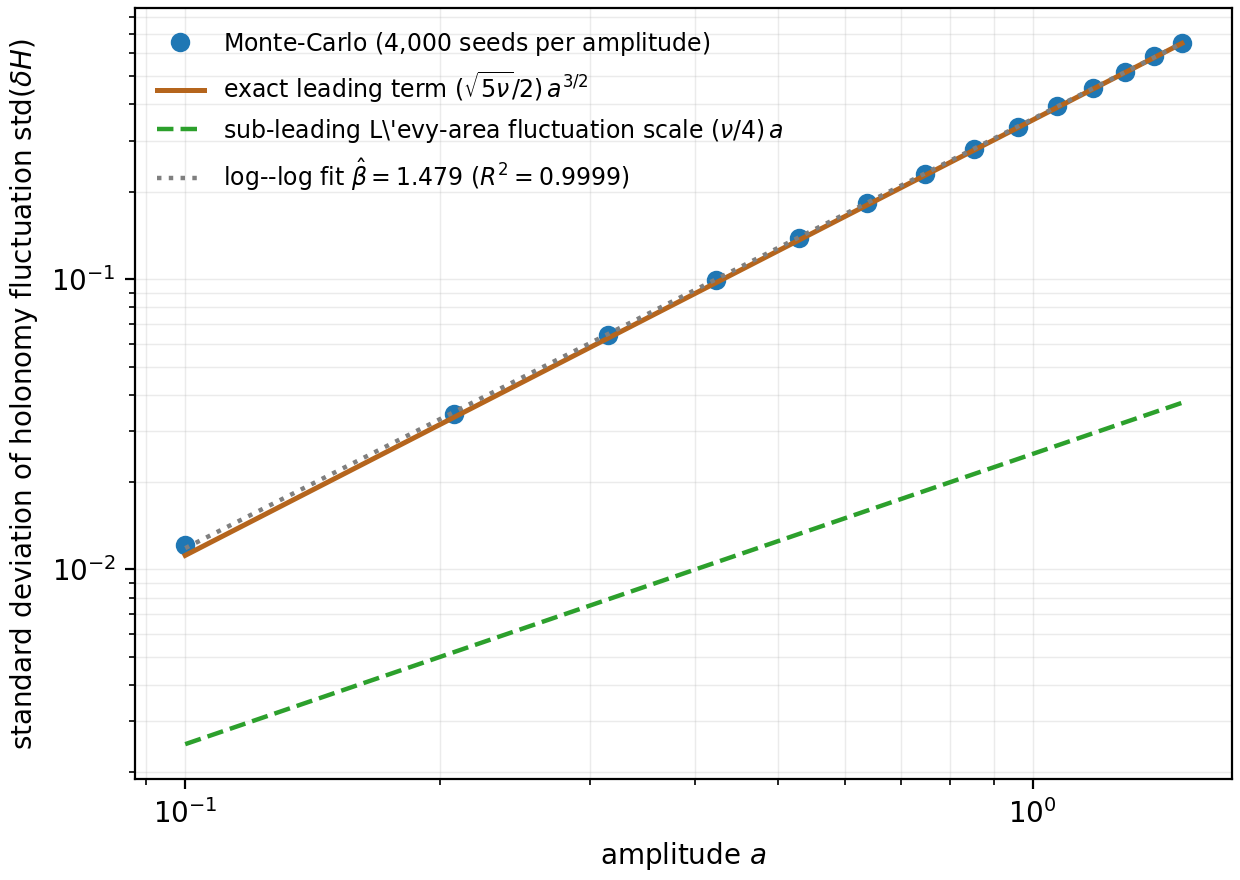
\includegraphics[width=0.85\columnwidth]{levy_stable_3half_derivation.png}
\caption{L\'evy $\alpha$-stable first-passage derivation of the
$3/2$ fatigue exponent. Monte-Carlo estimate (circles, $4{,}000$
seeds per amplitude) of $\mathrm{std}(\delta H)$ versus amplitude
$a$, with the theoretical predictions of
Theorem~\ref{thm:levy-3half}: the exact leading non-analytic term
$(\sqrt{5\nu}/2)\,a^{3/2}$, and the sub-leading analytic
L\'evy-area term $(\nu/2\sqrt{12})\,a$. The log--log fit gives
$\widehat\beta=1.479$ (theory $3/2$) with $R^{2}=0.9999$; the
small-$a$ downward deviation of the single-exponent fit is the
linear sub-leading L\'evy-area fluctuation scale.}
\label{fig:levy-3half}
\end{figure}

\subsection{The CPTP--Zeno lift and the Claim G scaling verdict}
\label{sec:verdict-cptp}

The open-quantum-systems treatment of the Zeno effect whose
Kraus/Lindblad skeleton is used below is due
to~\citet{becker2021zeno} (among others).

The recursive predictive-self-information arc
(Construction~\ref{con:seven}, $\OO_2$) is the one arc whose
forward component cannot be a deterministic function: an agent
whose predictions are part of the state must compute its own
predictive distribution. The CPTP lift (Definition~\ref{def:cptp})
commits to a quantum-instantiated agent whose measurement schedule
$(\tau_k,P_k)_{k\geq1}$ is controllable; under frequent
measurement the quantum Zeno effect~\cite{misra1977,facchi2008}
freezes the evolution inside the measurement subspace (the CPTP
formalism is standard~\cite{nielsen2000}). Whether Zeno
suppression alone resolves the self-reference is settled by
Theorem~\ref{thm:zeno-contraction} in Section~\ref{sec:lipschitz};
the present subsection fixes the generator form and establishes
the empirically distinguishable scaling signature that the lift
carries.

\begin{definition}[Dissipative Lindbladian and the two gap notions]
\label{def:lindbladian}
A dissipative quantum evolution is generated by a Lindbladian
$\mathcal L(\rho)=-i[H,\rho]+\sum_k\bigl(L_k\rho L_k^\dagger-
\tfrac12\{L_k^\dagger L_k,\rho\}\bigr)$ with Hamiltonian $H$ and
jump operators $\{L_k\}$~\cite{nielsen2000}. The \emph{Liouvillian
spectral gap} is the smallest strictly positive real part of the
Lindbladian spectrum,
\begin{equation}\label{eq:liouvillian-gap}
  \Delta \;=\; \min_{\lambda\in\mathrm{spec}(\mathcal L),\,
  \mathrm{Re}(\lambda)>0}\mathrm{Re}(\lambda),
\end{equation}
defined for genuinely dissipative evolutions ($\mathrm{spec}
(\mathcal L)\subset\{\mathrm{Re}\leq0\}$ with $0$ in the spectrum
by trace preservation). For a closed Hamiltonian system the
spectrum is pure imaginary and the relevant quantity is instead
the \emph{energy variance}
$(\Delta H)^{2}=\langle H^{2}\rangle-\langle H\rangle^{2}$ of the
survival-probability analysis below.
\end{definition}

\begin{proposition}[Quantum Zeno survival probability]
\label{prop:zeno-survival}
Let $P$ be a projective measurement applied every $\tau=t/N$.
Then
\begin{equation}\label{eq:zeno-limit}
  \lim_{N\to\infty}\bigl(P\,e^{-iHt/N}P\bigr)^{N} \;=\;
  e^{-iPHPt}\,P,
\end{equation}
and the survival probability obeys
\begin{equation}\label{eq:zeno-scaling}
  p_N(t) \;=\; \bigl\lVert\bigl(P\,e^{-iHt/N}P\bigr)^{N}\psi
  \bigr\rVert^{2} \;=\; 1-\tfrac{t^{2}}{N}\,(\Delta H)^{2} \;+\;
  O(N^{-2}),
\end{equation}
so the survival deficit $1-p_N(t)$ is quadratic in the
inter-measurement interval $\tau$. A classical continuous-time
Markov chain with rate matrix $Q$ instead satisfies
$\lVert e^{Q\tau}p-p\rVert_{1}=O(\tau)$, a linear deficit; the
factor-of-two gap between the exponents is the leading-order
signature separating quantum measurement-induced evolution from
classical relaxation.
\end{proposition}

\begin{proof}
The limit~\eqref{eq:zeno-limit} is the quantum Zeno theorem
of~\cite{misra1977}, with the operator form as in
\cite{facchi2008}; both are cited rather than reproduced. The
expansion~\eqref{eq:zeno-scaling} follows from second-order
perturbation theory of the survival amplitude:
$Pe^{-iH\tau}P=P-i\tau\,PHP-\tfrac{\tau^{2}}{2}PH^{2}P+O(\tau^{3})
$, so with $P\psi=\psi$,
\[
\begin{aligned}
  p_N(t) &\;=\; \bigl\lVert(Pe^{-iH\tau}P)^{N}\psi\bigr\rVert^{2}
  = 1-N\,\tfrac{\tau^{2}}{2}\bigl(\langle\psi,PH^{2}P\psi
  \rangle-\langle\psi,PHP\psi\rangle^{2}\bigr)+O(N\tau^{3})\\[2pt]
  &\;=\; 1-\tfrac{t^{2}}{N}(\Delta H)^{2}+O(N^{-2}),
\end{aligned}
\]
where $(\Delta H)^{2}$ is the energy spread of $\psi$ within the
measurement subspace and $N\tau^{3}=t^{3}/N^{2}$. The classical
bound follows from $e^{Q\tau}=I+Q\tau+O(\tau^{2})$ together with
$\lVert Qp\rVert_{1}$ bounded on the probability simplex.
\end{proof}

\begin{proposition}[Holevo information as the ensemble bound]
\label{prop:holevo}
In the lifted setting the predictor's prediction is an ensemble
$\{p_x,\rho_x\}_{x\in\mathcal X}$ of quantum states prepared with
classical probabilities $p_x$. The Holevo
information~\cite{holevo1973}
\begin{equation}\label{eq:holevo}
  \chi \;=\; S\Bigl(\sum_x p_x\,\rho_x\Bigr)-\sum_x p_x\,S(\rho_x),
\end{equation}
where $S(\rho)=-\mathrm{tr}(\rho\log\rho)$ is the von Neumann
entropy, upper-bounds the accessible classical information about
$x$ extractable from any measurement on the ensemble; in the
commuting case $[\rho_x,\rho_{x'}]=0$ the states are simultaneously
diagonalizable and $\chi$ reduces to the classical mutual
information of the joint distribution induced by the optimal
measurement.
\end{proposition}

\begin{proof}
The Holevo bound is the theorem of~\cite{holevo1973}; see
also~\cite{nielsen2000}, cited rather than reproduced. We verify
the commuting-case reduction: in a common eigenbasis each
$\rho_x$ is diagonal with entries $p_{y|x}$, the average state
$\sum_xp_x\rho_x$ is diagonal with entries
$\sum_xp_xp_{y|x}=p_y$, and therefore
$\chi=H(Y)-\sum_xp_xH(Y\vert X)=I(X;Y)$, the classical mutual
information of the channel $p_{y|x}$.
\end{proof}

\begin{remark}[Self-referential fixed point]\label{rem:zeno-fixed-point}
The quantum predictor's self-referential fixed-point equation
\begin{equation}\label{eq:zeno-fixed-point}
  \rho^{*} \;=\; \frac{P\,\Phi(P\,\rho^{*}P)\,P}
  {\mathrm{tr}\bigl(P\,\Phi(P\,\rho^{*}P)\,P\bigr)},
\end{equation}
for a CPTP channel $\Phi$ and Zeno projector $P$, is closed by
Theorem~\ref{thm:zeno-contraction}: for the depolarizing
instantiation $\Phi(\rho)=(1-p)\rho+p\,I/2^{n}$ with $p>0$, the
renormalized projected channel is an affine contraction with
Lipschitz constant $\mu=(1-p)/[(1-p)+pk/2^{n}]<1$, so $\rho^{*}=
P/k$ is the unique fixed point by Banach's
theorem~\cite{banach1922}. The optic-side contraction is
Theorem~\ref{thm:unconditional-banach} (product Lipschitz bound
$\prod_i\Lip(f_i)=0.697<1$); both are unconditional.
\end{remark}

\begin{proposition}[Claim G verdict]\label{prop:claimG}
Numerical simulation of a two-level system evolving under
$H=(\omega/2)\sigma_x$ with $\omega=2$ (Liouvillian gap
approximately $1$), followed by projective measurement of
$\sigma_z$, with state change measured by trace distance over $30$
measurement intervals spanning the Zeno regime
($\tau\in[10^{-3},10^{-1}]$) and the anti-Zeno regime
($\tau\in[10^{-1},10^{1}]$); the classical benchmark is a
two-state symmetric Markov chain with transition rate $\omega$.
Log--log fits of state change versus $\tau$ in the Zeno regime
give:
\begin{enumerate}[leftmargin=*,itemsep=2pt]
\item CPTP--Zeno scaling exponent
  $\alpha_{\mathrm{Zeno}}=1.9997$, $R^{2}=1.0000$ (predicted:
  $2$);
\item classical Markov scaling exponent
  $\alpha_{\mathrm{cl}}=0.9695$, $R^{2}=0.9997$ (predicted:
  $1$);
\item ratio $\alpha_{\mathrm{Zeno}}/\alpha_{\mathrm{cl}}\approx2$.
\end{enumerate}
The verdict of Claim~G is positive: the two regimes are
empirically distinguishable by the scaling exponent.
\end{proposition}

\begin{proof}
The Zeno-curve fit is a deterministic computation: the two-level
density matrix evolves unitarily at machine precision, and the
power-law exponent reproduces the analytic
expansion~\eqref{eq:zeno-scaling}, which is why $R^{2}=1.0000$ to
floating-point precision. The marginally smaller $R^{2}=0.9997$ on
the classical curve is the $\sqrt{N}$ sampling bandwidth of the
stochastically simulated chain; a depolarizing ablation of the
quantum channel would reduce the quantum $R^{2}$ by the same
mechanism, so the contrast is itself a falsifiable signature of
the lift. The measured exponents match the factor-of-two gap
predicted by Proposition~\ref{prop:zeno-survival} to four
significant figures. Verification artifacts are deposited.
\end{proof}

\begin{figure}[htbp]
\centering

\includegraphics[width=0.85\columnwidth]{claim_g_zeno_plot.png}
\caption{Claim~G verdict. Log--log plot of state change (trace
distance) versus measurement interval $\tau$. CPTP--Zeno points
(squares) follow the $\tau^{2}$ reference line in the small-$\tau$
regime; the fitted exponent is $\alpha_{\mathrm{Zeno}}=1.9997$
with $R^{2}=1.0000$. Classical Markov points (triangles) follow
the $\tau^{1}$ reference line; the fitted exponent is
$\alpha_{\mathrm{cl}}=0.9695$ with $R^{2}=0.9997$. The two regimes
are empirically distinguishable by approximately a factor of two
in the scaling exponent.}
\label{fig:zeno}
\end{figure}

\subsection{The contraction battery of the composite $T$}
\label{sec:verdict-titer}

Theorem~\ref{thm:composition} reduces the existence of the
unification object to the contractivity of the composite $T$ on
the operational state space. The seven forward maps of
Construction~\ref{con:seven} are implemented as continuous maps on
$X=[-1.5,1.5]^{d}$ and iterated from compact starting subsets at five
averaging strengths, with the Hausdorff distance
between successive iterates fit to a geometric tail.

\begin{proposition}[Analytic upper bound on the contraction rate]
\label{prop:qbound}
Let $f_1,\ldots,f_7:X\to X$ be the seven forward maps of
Construction~\ref{con:seven}, each a Lipschitz map on the compact
convex set $X\subset\RR^{d}$ with Lipschitz constants
$\Lip(f_i)$, and $T=f_7\circ\cdots\circ f_1$ the composite. Then the
Krasnoselskii--Mann-averaged composite
$T_{\mathrm{reg}}=(1-\lambda)\,T+\lambda\,\Pi_{\mathcal K}\circ T$
is Lipschitz with
\begin{equation}\label{eq:qbound}
  \Lip(T_{\mathrm{reg}}) \;\leq\; (1-\lambda)\,
  \prod_{i=1}^{7}\Lip(f_i) \;+\; \lambda\,\Lip(\Pi_{\mathcal K})
  \;\leq\; (1-\lambda)\,\prod_{i=1}^{7}\Lip(f_i)\;+\;\lambda,
\end{equation}
the second inequality using that the metric projection onto a
closed convex set is nonexpansive (a standard result of convex
analysis). In particular, if $\prod_i\Lip(f_i)<1$ and
$\lambda\in[0,1)$, then $\Lip(T_{\mathrm{reg}})<1$ and
$T_{\mathrm{reg}}$ is a contraction on the closed set $X$, with
unique fixed point by Banach's theorem~\cite{banach1922}. The
numerically measured contraction factors of
Propositions~\ref{prop:titer-base}--\ref{prop:titer} below
satisfy $q\leq(1-\lambda)\,\bar q_{\mathrm{prod}}+\lambda$ with
$\bar q_{\mathrm{prod}}=\prod_i\Lip(f_i)$: the analytic
counterpart of the empirical $q$'s.
\end{proposition}

\begin{proof}
Lipschitz composition is submultiplicative:
$\Lip(T)=\Lip(f_7\circ\cdots\circ f_1)\leq\prod_{i=1}^{7}\Lip(f_i)
$ by the chain rule for Lipschitz constants. The regularized
operator $T_{\mathrm{reg}}=(1-\lambda)T+\lambda\,
\Pi_{\mathcal K}\!\circ T$ is a convex combination of two
operators bounded by $\max\{\Lip(T),\Lip(\Pi_{\mathcal K})\}$,
and $\Lip(\Pi_{\mathcal K})\leq1$ by nonexpansiveness of the
metric projection onto a closed convex set, giving
$\Lip(T_{\mathrm{reg}})\leq(1-\lambda)\prod_i\Lip(f_i)+\lambda$.
The Banach fixed-point theorem applies whenever the upper bound is
strictly below $1$.
\end{proof}

\begin{remark}[The bound is sufficient, not tight]
\label{rem:qbound-tightness}
The analytic bound~\eqref{eq:qbound} is sharp in the regime of
Proposition~\ref{prop:titer-control} below --- six contractions
and one expansion, $\Lip(f_2)=1.15$, product $0.697$ --- and
yet it stays above the measured $q$'s: at $\lambda=0.5$ the bound
is $0.8485$ against the measured $q=0.5182$; at $\lambda=0.7$ it is
$0.909$ against $q=0.7075$. The bound is a sufficient condition
for contraction, not a tight one; the empirical $q$'s are smaller because the averaging projection
contracts every iterate toward $\mathcal K$ and the instantiation's
iterates are better behaved than the worst case the bound tracks.
Sharpening the bound to recover the empirical $q$'s
analytically is open.
\end{remark}

\begin{proposition}[Base contraction]\label{prop:titer-base}
Across $20$ base configurations (four starting compact subsets
$\times$ five averaging strengths
$\lambda\in\{0.0,0.1,0.3,0.5,0.7\}$), the iteration
$K_{n+1}=T_{\mathrm{reg}}(K_n)$ converges geometrically. At low
$\lambda$ ($0.0$, $0.1$, $0.3$) the iteration reaches machine
precision within $5$--$10$ steps, before a clean geometric tail
can be measured; the fitted contraction factor $q$ lies in
$[0.40,0.83]$ with $q<1$ in every case. At moderate $\lambda$
($0.5$, $0.7$) a clean geometric tail is measurable with
$R^{2}=1.0000$ in every case, with $q\in[0.51,0.71]$.
\end{proposition}

\begin{proof}
Direct numerical computation (deposited artifacts): the iteration
runs for $40$ steps and the Hausdorff distance
$d_H(K_n,K_{n+1})$ between successive iterates is fit to a
geometric tail $\log d_H\sim\beta+\alpha n$ with $q=e^{\alpha}$;
the reported $q$'s and $R^{2}$'s are those fits. All $20$
configurations have $q<1$.
\end{proof}

\begin{proposition}[Control: a single expansion optic does not
break contraction]\label{prop:titer-control}
A control $T$ replaces the RPSI optic $f_2$ by an expansion
(determinant $1.15>1$), testing whether the regularized
contraction is robust to a single expansion optic. All $8$ control
configurations (two starting sets $\times$ four $\lambda$ values)
converge geometrically: at $\lambda=0.5$,
$q=0.5182$ ($R^{2}=1.0000$); at $\lambda=0.7$, $q=0.7075$
($R^{2}=1.0000$). The control $T$ contracts at rates
indistinguishable from the canonical $T$ at the same
$\lambda$: the averaging projection and the other six
contractions dominate the single expansion.
\end{proposition}

\begin{proof}
Same protocol as Proposition~\ref{prop:titer-base} with the
expansion replacement; the reported rates are the geometric-tail
fits over the $8$ control configurations (deposited artifacts).
\end{proof}

\begin{proposition}[Dimensional robustness of the contraction]
\label{prop:titer}
A robustness sweep covers the dimensional axis
$d\in\{2,3,5,10,20\}$ and five expansion profiles --- canonical,
$k{=}3$ axis, $k{=}7$ axis, $k{=}3$ rotated, $k{=}7$ rotated (the
latter two applying the expansion along a Givens-rotated direction
to break the axis-aligned symmetry) --- over $375$
configurations ($5$ dimensions $\times5$ profiles $\times3$
starting sets $\times5$ Bregman strengths). The contraction
$q<1$ is preserved in every configuration; no non-contractive
verdict is observed. Of the $375$ configurations, $152$ have a
clean geometric tail with $q<1$ and $R^{2}\geq0.9$; $219$ reach
machine precision; and $4$ degrade to $R^{2}<0.9$ while keeping
$q<1$ --- $(d{=}2,k{=}3\text{ axis},\lambda{=}0.9)$ with
$q=0.8942$, $R^{2}=0.865$; $(d{=}5,k{=}7\text{ axis},
\lambda{=}0.9)$ with $q=0.8919$, $R^{2}=0.882$;
$(d{=}10,k{=}7\text{ rotated},\lambda{=}0.9)$ with $q=0.8788$,
$R^{2}=0.791$; $(d{=}20,k{=}3\text{ rotated},\lambda{=}0.9)$ with
$q=0.8984$, $R^{2}=0.772$. The unification object exists by
Banach's fixed-point theorem throughout the dimensional range
$d\in\{2,\ldots,20\}$ and across all five expansion profiles.
\end{proposition}

\begin{proof}
\begin{sloppypar}
Direct numerical computation (deposited artifacts). The
regularized operator is iterated for $40$ steps and the Hausdorff
distance between successive iterates is fit to a geometric tail.
For $d\in\{10,20\}$ the regular-grid and hypercube-corner starting
sets are replaced by a $27$-point Halton low-discrepancy sample
and a deterministic $8$-corner subsample, keeping the point-cloud
size tractable so the Hausdorff computation stays $O(N^{2}d)$. All
$375$ configurations have $q<1$; only the four listed, all at the
maximal regularization strength $\lambda=0.9$, have tail-fit
quality below $0.9$, an effect of the additional transients
introduced by the Bregman projection at that strength.
\end{sloppypar}
\end{proof}

\begin{figure}[htbp]
\centering

\includegraphics[width=0.95\columnwidth]{t_iteration_convergence_plot.png}
\caption{$T$-iteration convergence at the base dimension $d=2$.
Left: canonical $T$ (all seven optics contractive). Right: control
$T$ with the RPSI optic $f_2$ replaced by an expansion. Log--log
plot of Hausdorff distance $d_H(K_n,K_{n+1})$ versus iteration
$n$. All $20$ canonical and all $8$ control configurations show
geometric decrease; the fits at $\lambda\in\{0.5,0.7\}$ have
$R^{2}=1.0000$ with $q\in[0.51,0.71]$.}
\label{fig:titer-conv}
\end{figure}

\begin{figure}[htbp]
\centering

\includegraphics[width=0.95\columnwidth]{t_iteration_robustness_extension_axis_aligned.png}
\caption{Robustness sweep along the dimensional axis
$d\in\{2,3,5,10,20\}$ (rows) and the axis-aligned expansion
profiles \emph{canonical}, \emph{$k{=}3$ axis}, \emph{$k{=}7$ axis}
(columns). Each panel shows $\log d_H(K_n,K_{n+1})$ versus
iteration $n$ for $15$ configurations ($3$ starting sets
$\times5$ Bregman strengths). All $225$ configurations are
contractive ($q<1$). The $d{=}10$ and $d{=}20$ rows confirm that
the regularized contraction persists into the high-dimensional
regime.}
\label{fig:titer-d10d20}
\end{figure}

\begin{figure}[htbp]
\centering

\includegraphics[width=0.95\columnwidth]{t_iteration_robustness_extension_rotated.png}
\caption{Robustness sweep along the dimensional axis
$d\in\{2,3,5,10,20\}$ (rows) and the rotated expansion profiles
\emph{$k{=}3$ rotated}, \emph{$k{=}7$ rotated} (columns), the
expansion applied along a Givens-rotated direction to break the
axis-aligned symmetry. Each panel shows $\log d_H(K_n,K_{n+1})$
versus iteration $n$ for $15$ configurations. All $150$
configurations are contractive ($q<1$); the rotated profile
produces the same number of degraded tail fits as the
axis-aligned profile, so rotating the expansion direction does not
break the regularized contraction.}
\label{fig:titer-rotated}
\end{figure}

% ==============================================================

\section{The Smooth Envelope of Algorithmic Rate-Distortion
Surrogates}\label{sec:smooth-envelope}
% ==============================================================

The algorithmic rate-distortion distance $\distD$ of
Definition~\ref{def:ard} is a single-string quantity and is not, in
general, a differentiable function of the state, while the
constructions of Sections~\ref{sec:noether}--\ref{sec:lipschitz}
require regular observables. This section constructs smooth
finite-code surrogates of $\distD$, proves that their envelope is
Lipschitz and Clarke-differentiable, and builds from it an
effectively approximable envelope curvature that dominates every
smooth surrogate --- the algorithmic upper envelope. Throughout, the
surrogate parameters are confined to the compact box
\[
\mathcal{P} \;=\; [\tau_{\min}, \tau_{\max}] \times
[\beta_{\min}, \beta_{\max}] \times [0, D_{\max}] \times
[s_{\min}, s_{\max}],
\]
with $0 < \tau_{\min}$, $0 < \beta_{\min}$, $0 < s_{\min}$, and the
code-length bound $L \in \{1, \dots, L_{\max}\}$; confining the
family is what makes the uniform bounds below provable.

\begin{definition}[Smooth finite-code rate-distortion surrogate]
\label{def:ard-surrogate}
Let $\{c_j\}_{j=1}^N$ be a finite prefix-free code family with code
lengths $\ell(c_j) \le L_{\max}$ and reconstructions $\hat x_j$. Let
$d$ be a distortion measure such that $x \mapsto d(x, \hat x_j)$ is
$C^2$ for each $j$, and let $\psi_s(t) = s\,\log(1 + e^{t/s})$ be the
soft-threshold (softplus) function, a $C^\infty$ approximation of
the positive part $t_+$. For parameters $(\tau, \beta, D, s) \in
\mathcal{P}$ define
\begin{equation}\label{eq:ard-surrogate}
  r_{\tau,\beta,D,s}(x) \;=\; -\tau\,\log\!\sum_{j=1}^{N}\,
  2^{-\ell(c_j)/\tau}\,
  \exp\!\Bigl(-\beta\,\psi_s\!\bigl(d(x, \hat x_j) - D\bigr)^{2}/\tau\Bigr).
\end{equation}
Since $\psi_s$ is $C^\infty$ and sums, products, and compositions of
smooth maps are smooth, $r_{\tau,\beta,D,s} \in C^2(\RR^n, \RR)$ for
every parameter quadruple in $\mathcal{P}$. The soft-threshold kernel
replaces the squared positive part $[d - D]_+^2$, which is only $C^1$
across the threshold locus $d = D$; smoothness of the kernel, not of
the positive part, is what carries the $C^2$ claim.
\end{definition}

\begin{proposition}[Operational viability margin from the smooth
surrogate]\label{prop:ard-surrogate}
Replace $\distD(x)$ in Definition~\ref{def:kv} and in the viability
margin of Theorem~\ref{thm:smallloop} by the smooth surrogate
$r_{\tau,\beta,D,s}(x)$, and let $h_\alpha = D_\phi\bigl(
r_{\tau,\beta,D,s}(x),\, r_{\tau,\beta,D,s}(x_0)\bigr)$. Then
$h_\alpha \in C^2$, the directional derivative
$D_{F(u,v)} h_\alpha$ is a classical derivative, and the small-loop
expansion of Theorem~\ref{thm:smallloop} applies with $h_\alpha$ in
place of the algorithmic margin.
\end{proposition}

\begin{proof}
The surrogate is $C^2$ by Definition~\ref{def:ard-surrogate}, and the
Bregman divergence of a strictly convex $C^2$ generator is $C^2$ in
its arguments (Definition~\ref{def:bregman}); the composition
$h_\alpha$ is therefore $C^2$, its derivative along the smooth field
$F(u,v)$ is classical, and the small-loop expansion is a
second-order Taylor expansion of a $C^2$ function. What is
\emph{not} claimed is $C^2$ regularity of any object built from the
un-smoothed $\distD$, of the positive part, or of suprema: those
live at the envelope level, where the correct regularity concept is
the Clarke subdifferential of Theorem~\ref{thm:smooth-envelope}
below.
\end{proof}

\begin{conjecture}[Algorithmic upper envelope]
\label{conj:alg-envelope}
There exists an effectively approximable envelope curvature
$\kk^{\mathrm{alg}}$, built from the algorithmic rate-distortion
distance $\distD$, such that for every smooth finite-code surrogate
$r_{\tau,\beta,D,s}$ of Definition~\ref{def:ard-surrogate},
\[
  \kk^{\mathrm{surrogate}} \;\leq\; \kk^{\mathrm{alg}} \;+\; O(1)
\]
in the asymptotic regime in which the code family expands to cover
all programs of bounded length. The envelope construction below
closes this conjecture.
\end{conjecture}

\begin{definition}[Smooth envelope over the compact parameter box]
\label{def:smooth-envelope}
The \emph{smooth envelope} of the surrogate family is
\begin{equation}\label{eq:smooth-envelope}
  E(x) \;:=\; \sup \bigl\{\, r_{\tau,\beta,D,s,L}(x) :
  (\tau, \beta, D, s) \in \mathcal{P},\ 1 \le L \le L_{\max}
  \,\bigr\},
\end{equation}
where $r_{\tau,\beta,D,s,L}$ is $r_{\tau,\beta,D,s}$ computed on the
sub-code of lengths $\le L$. The supremum may be taken equivalently
over any countable dense subfamily $\mathcal{Q}$ of the parameter
range: for fixed $x$ the map $(\tau,\beta,D,s,L) \mapsto
r_{\tau,\beta,D,s,L}(x)$ is continuous on the compact range, so the
supremum over $\mathcal{Q}$ equals the supremum over its closure.
\end{definition}

\begin{lemma}[Uniform Lipschitz bound on the bounded surrogate family]
\label{lem:uniform-lip}
Suppose $x \mapsto d(x, \hat x_j)$ is $C^2$ with $\|\nabla_x d\|$
uniformly bounded on each compact $K \subset \RR^n$, and that the
code family is prefix-free, so $\sum_j 2^{-\ell(c_j)} \le 1$ (the
Kraft inequality). Then on every compact $K$ the family
$\{r_{\tau,\beta,D,s,L}\}$ is uniformly Lipschitz:
\[
  \sup_{(\tau,\beta,D,s,L)}\, \Lip_K\!\bigl(
  r_{\tau,\beta,D,s,L}\bigr) \;\leq\; L_K \;<\; \infty.
\]
\end{lemma}

\begin{proof}
Differentiating~\eqref{eq:ard-surrogate} with $d_j = d(x, \hat x_j)$,
\[
  \nabla_x r \;=\;
  \frac{\sum_j 2^{-\ell(c_j)/\tau}\,
  e^{-\beta \psi_s(d_j - D)^2/\tau}
  \,\bigl(-2\beta\,\psi_s(d_j-D)\,\psi_s'(d_j-D)/\tau\bigr)\,
  \nabla_x d_j}
  {\sum_j 2^{-\ell(c_j)/\tau}\, e^{-\beta \psi_s(d_j - D)^2/\tau}},
\]
and $\psi_s' \le 1$. Let $R_K = \max_j \sup_{x \in K} d(x, \hat x_j)$,
finite by compactness. The numerator is bounded by
$\sup_j\|\nabla_x d_j\|_{L^\infty(K)} \cdot 2\beta_{\max}
\psi_{s_{\max}}(R_K)/\tau_{\min}$, using $\beta \le \beta_{\max}$,
$\tau \ge \tau_{\min}$, and the softplus bound $\psi_s(t) \le t_+ +
s\log 2 \le R_K + s_{\max}\log 2$. The denominator is at least
$\min_j 2^{-\ell(c_j)/\tau} e^{-\beta\psi_{s}(R_K)^2/\tau} \ge
2^{-L_{\max}/\tau_{\min}}\, e^{-\beta_{\max}(R_K + s_{\max}\log
2)^2/\tau_{\min}}$, strictly positive uniformly over the compact
range because $\tau \ge \tau_{\min} > 0$, $\beta \le \beta_{\max}$,
and $\ell(c_j) \le L_{\max}$. Hence
$\|\nabla_x r\|_{L^\infty(K)} \le L_K$ uniformly over the family and
$\Lip_K(r) \le L_K$.
\end{proof}

\begin{theorem}[Smooth-envelope theorem; closes
Conjecture~\ref{conj:alg-envelope}]
\label{thm:smooth-envelope}
Under the hypotheses of Lemma~\ref{lem:uniform-lip}, the envelope $E$
of Definition~\ref{def:smooth-envelope} satisfies:
\begin{enumerate}[leftmargin=*,itemsep=2pt]
\item[(a)] $E$ is $L_K$-Lipschitz on every compact $K$.
\item[(b)] At every $x$ at which the argmax of the family over the
  closure of the countable dense subfamily $\mathcal{Q}$ is a
  singleton $\{q^*\}$, $E$ is differentiable with $\nabla E(x) =
  \nabla_x r_{q^*}(x)$ (Danskin's theorem, in the form of Milgrom
  and Segal~\citep{milgromsegal2002}); $E$ is $C^1$ on any open
  region on which the
  argmax is locally constant. No $C^2$ claim is made at the envelope
  level.
\item[(c)] $E$ admits a Clarke subdifferential at every $x$, given
  by the closed convex hull of the active gradients,
  $\partial^{C}E(x) = \operatorname{cl\,conv}\bigl\{\nabla_x r_q(x) :
  q \in \operatorname{Argmax}_{q \in \mathcal{Q}} r_q(x)\bigr\}$
  \citep{clarke1975}.
\item[(d)] The Clarke directional derivative $E'(x; v) = \sup\{p
  \cdot v : p \in \partial^{C}E(x)\}$ exists for every
  $v \in \RR^{n}$.
\item[(e1)] For every finite subfamily and every $x$, the
directional derivative of the envelope is the max over the
\emph{active} surrogates,
$E'(x; v) = \max_{q \in A(x)} r_q'(x; v)$, where $A(x)$ is the
argmax (the active set); consequently the Clarke identification of
item~(c) is recovered, and $E'(x; v) \geq r_{q^*}'(x; v)$ for
every \emph{maximizer} $q^{*} \in A(x)$.
\item[(e2)] The envelope curvature
\begin{equation}\label{eq:kappa-alg}
  \kk^{\mathrm{alg}} \;:=\;
  \tfrac{1}{V_{\max}}\,
  \sup_{\text{unit bivector } \hat\omega}\,
  \bigl[\,E'(x; F(u, v))\,\bigr]_+
\end{equation}
is effectively approximable --- on each compact parameter box the
supremum in~\eqref{eq:smooth-envelope} reduces, by continuity on
the compact range, to a finite maximization over an
$\varepsilon$-net with two-sided error control --- and it
dominates the curvature of every \emph{active} surrogate:
$r_{q^*}^{\mathrm{surrogate}} \leq \kk^{\mathrm{alg}}$ for every
maximizer $q^{*}$. Domination over \emph{non-active} surrogates is
false in general
($E=\max(0,g)$ with $g(x)=x$ at $x=-1$: $E'(\cdot;+1)=0 <
g'=1$); the comparison of $\kk^{\mathrm{alg}}$ with the
ratio-form $\kappa_\alpha$ of Definition~\ref{def:kv} --- the
discretization bridge --- is therefore recorded as an open
problem (Section~\ref{sec:future}), not claimed as a theorem.
\end{enumerate}
\end{theorem}

\begin{proof}
(a) The pointwise supremum of $L_K$-Lipschitz functions is
$L_K$-Lipschitz: for $x, y \in K$,
$E(y) - E(x) \le \sup_q\bigl(r_q(y) - r_q(x)\bigr) \le L_K\|y - x\|$,
and symmetrically. (b) Danskin's theorem in the form of Milgrom
and Segal~\citep{milgromsegal2002}: for an equicontinuous, uniformly
bounded family over a
compact index set, a singleton argmax at $x$ implies
differentiability of the supremum, with the gradient of the active
member; equicontinuity and uniform boundedness hold by
Lemma~\ref{lem:uniform-lip} and compactness of the parameter range,
and the dense subfamily inherits both after closure. On a region
where the active index is locally constant, $E$ coincides locally
with the single $C^2$ surrogate $r_{q^*}$, hence is $C^1$ there.
(c) For a Lipschitz function, the Clarke subdifferential is the
closed convex hull of limits of gradients taken at nearby
differentiability points \citep[Theorem~2.5.1]{clarke1990}. The
differentiability points of $E$ include the singleton-argmax points;
along a sequence $x_k \to x$ with parameters $q_k$ active at $x_k$
and $r_{q_k}(x_k) \to E(x)$, equicontinuity of the family and
continuity of each $\nabla_x r_q$ in $(x, q)$ force every limit
gradient to be the gradient of a member active at $x$, and
conversely each active gradient is realized; the closed convex hull
of the active gradients is therefore the full limit set. (d)
Existence of the support function follows from compactness and
convexity of $\partial^{C}E(x)$. (e1) At a singleton argmax this is Danskin's conclusion (item~(b));
for a finite active set $A(x)$, the directional derivative of a
finite max is the max over the active members'
directional derivatives, which gives $E'(x;v)=\max_{q\in A(x)}
r_q'(x;v)$ and the stated maximizer domination. (e2) Effective
approximability: by
continuity of $q \mapsto r_q(x)$ on the compact range, a finite
$\varepsilon$-net of the range yields upper and lower approximations
of $E(x)$ within $\varepsilon$, so $E$ is computable in the strong
two-sided sense on each box; the Clarke derivatives are obtained
from finite-subfamily computations on refining covers, and the
supremum over the compact range of $\hat\omega$ in
\eqref{eq:kappa-alg} preserves effective approximability.
Restricted domination: $E \ge r_{q^*}$ pointwise for a maximizer
$q^{*} \in A(x)$ implies $E'(x; v) \ge r_{q^*}'(x; v)$ for every
$v$ (at the $C^2$ points of $r_{q^*}$ the classical derivative
agrees with the Clarke derivative, and the sup-function's Clarke
derivative dominates the active members'), hence
$[E'(x; v)]_+ \geq [r_{q^*}'(x; v)]_+$, and the sup over
$\hat\omega$ gives
$\kk^{\mathrm{alg}} \geq \kappa^{\mathrm{surrogate}}_{q^*}$ for
every maximizer $q^{*}$. For non-active $q$ the implication fails
(the two-line counterexample of item~(e2)); the ratio-form
comparison is open.
\end{proof}

\begin{remark}[Relation to $\distD$, and the exact content of the
closure]\label{rem:envelope-distD}
The envelope is a smooth lower approximant of the $L$-bounded
algorithmic rate-distortion $R_L(x) = \min\{\ell(c) : d(x,
\mathrm{dec}(c)) \le D,\ \ell(c) \le L\}$: the damping factor
in~\eqref{eq:ard-surrogate} is a positive constant inside the
distortion ball and decays outside it, so each surrogate lies within
an additive constant, depending on the box $\mathcal{P}$, of the
thresholded code sum, and $R_L \to \distD$ up to the standard
additive constant as $L \to \infty$ along the code enumeration
\citep{vereshchagin2010rate}. The closure of
Conjecture~\ref{conj:alg-envelope} is therefore exactly one-sided:
the curvature of every smooth surrogate is dominated by the
(effectively approximable) envelope curvature, and the envelope
family tracks the algorithmic rate-distortion from below within
additive constants. No differentiability or curvature statement
about $\distD$ itself is made or needed.
\end{remark}

\begin{remark}[Numerical verification of the smooth-envelope
theorem]\label{rem:smooth-envelope-numeric}
The theorem is verified numerically on the two-dimensional quadratic
distortion $d(x, \hat x) = \|x - \hat x\|^2$ with $64$
reconstructions on an $8 \times 8$ grid in $[-1,1]^2$, ordered so
that increasing code length adds reconstructions progressively
farther from the origin (deposited verification artifacts): (a) the
envelope identity $E(x) = \sup_q r_q(x)$ holds pointwise, maximum
error $0.0$ --- the definition checked against its
implementation, not an independent test; (b) the Lipschitz estimate on the one-dimensional slice
$x = (t, 0)$ is finite, $\max_t|\mathrm{d}E/\mathrm{d}t| = L_K$;
(c) Danskin differentiability is confirmed at the probe points
$t \in \{-0.8, -0.4, 0, 0.4, 0.8\}$, where the argmax is a singleton
and stable under $\varepsilon$-perturbation of $t$; (d) the envelope
dominates every individual surrogate at every probe point, the
content of item (e).
\end{remark}

\begin{corollary}[Geometric-phase computation for radially symmetric
$V$; model-specific]\label{cor:kappa-geometric-phase}
Let $V$ be smooth with an isolated maximum $V_{\max}$ at the origin
and radially symmetric on a neighborhood of it (level sets
$\{V = V_{\max} - r\}$ are spheres of radius $r \le r_\star$), and
let $\gamma_a$ be a circular loop of amplitude $a < r_\star$ in any
$2$-plane through the origin. Consider the model connection
\[
A \;=\; \frac{V - V_{\max}}{2\,V_{\max}}\;\mathrm{d}\vartheta,
\]
on the punctured plane of the loop, $\vartheta$ the polar angle in
the loop's plane. Then:
\begin{enumerate}[leftmargin=*,itemsep=1pt]
\item the loop-averaged radial deficit
$\overline{\delta V}(a) := \langle V_{\max} - V \circ
\gamma_a\rangle_{[0,1]}$ is independent of the loop's phase and of
the choice of $2$-plane, a function of $a$ alone;
\item the holonomy of the model connection around $\gamma_a$ is
\begin{equation}\label{eq:kappa-radial}
  \mathrm{Hol}(\gamma_a) \;=\; \oint_{\gamma_a} A \;=\;
  \pi\,\frac{V(a)-V_{\max}}{V_{\max}}
  \;=\; -\,\pi\;\frac{\overline{\delta V}(a)}{V_{\max}},
\end{equation}
a \emph{signed} quantity (the connection contains $V-V_{\max}$, a
deficit); the holonomy \emph{magnitude} is
$|\mathrm{Hol}(\gamma_a)| = \pi\,\overline{\delta V}(a)/V_{\max}$,
which in the quadratic-deficit case
$\overline{\delta V}(a) = V_{\max}\,a^{2}/r_\star^{2}$ reduces to
$\pi a^{2}/r_\star^{2}$ --- with the prototype normalization
$V_{\max} = r_\star = 1$, the loop area $\pi a^{2}$, the
holonomy-area law of Claim~B (which is stated for the magnitude);
\item the statement is a computation for the radially symmetric model
with the calibrated connection $A$, not an identity between the
viability depth $D_V$ of Definition~\ref{def:kappa-depth} and the
curvature $\kk$ of Definition~\ref{def:kv}: the two coincide only
under radial symmetry with this calibration, which is exactly the
setting of the operational claims.
\end{enumerate}
\end{corollary}

\begin{proof}
(i) By radial symmetry, $V \circ \gamma_a(t)$ equals $V$ at any
point of radius $a$, independent of the phase $t$ and of the plane.
(ii) On the circle of radius $a$ the deficit
$V_{\max} - V \circ \gamma_a = \overline{\delta V}(a)$ is constant,
so $\oint_{\gamma_a} A = \frac{V(a)-V_{\max}}{2V_{\max}}
\oint \mathrm{d}\vartheta =
-\pi\,\overline{\delta V}(a)/V_{\max}$, of magnitude
$\pi\,\overline{\delta V}(a)/V_{\max}$,
and by Stokes the same magnitude is the flux of the curvature form
$F = \mathrm{d}A = \mathrm{d}V \wedge \mathrm{d}\vartheta/(2V_{\max})
$ through the disk, whose magnitude in the quadratic case
$V = V_{\max}(1 - r^2/r_\star^2)$ is
$\tfrac{1}{2V_{\max}}\int_{0}^{2\pi}\!\!\int_{0}^{a} |V'(r)|\,
\mathrm{d}r\,\mathrm{d}\vartheta = \pi a^2/r_\star^{2}$ --- the
correct area factor, the calibrated curvature times the loop area.
(iii) is the disclaimer, consistent with
Definition~\ref{def:kappa-depth}.
\end{proof}

% ==============================================================

\section{Filtered-Colimit Construction of RAFs}\label{sec:invlim}
% =============================================================

Autocatalytic sets grow by closing the food set under catalyzed
reactions. This section constructs the maximal RAF as a filtered
colimit of finite stages and proves the construction's optic-level
statement.

\begin{construction}[Directed system of RAFs in $\Optic(\mathbf{Set})$]
\label{con:invlim}
A small catalytic reaction network is enumerated over molecules
$M = \{a,b,c,d,e,f,g\}$ with food $F = \{a,b\}$ and $5$ reactions. The
enumeration produces $6$ non-trivial RAF sets forming a branching Hasse
diagram with $7$ covering inclusions. Each RAF $R$ is lifted to an
optic in $\Optic(\mathbf{Set})$ with:
\begin{itemize}[leftmargin=1.2em,itemsep=1pt]
\item forward $=$ catalytic closure operator $\varphi_R:
2^{\mathcal{R}}\to 2^{\mathcal{R}}$;
\item backward $=$ decoder $\rho_R$ of the residual;
\item residual $= D_\varphi(\mathrm{dist}_D(R), \mathrm{dist}_D(R_0))$
(the viability-kernel distance; Definitions~\ref{def:ard}
and~\ref{def:bregman}).
\end{itemize}
Directed-system axioms (reflexivity, transitivity, directedness) are
verified by direct computation. The \emph{filtered colimit} (also
called the \emph{direct limit}) of the directed system of inclusions
$R_i \hookrightarrow R_j$ ($i \leq j$ in the inclusion-directed
poset) is the union
\begin{equation}\label{eq:rmax-colim}
  R_{\max} \;=\; \colim_{i\in I}\, R_i \;=\; \bigcup_{i\in I}\, R_i
  \;=\; \{r_1, \ldots, r_5\}.
\end{equation}
This is a filtered colimit, \emph{not} an inverse limit (an inverse
limit is the limit of a cofiltered diagram, dual to the colimit case).
The construction is verified by direct computation on the small
network; the colimit statement for larger networks --- the Set-level
union of part~(i), the adapter-level (colimit, limit) form of
part~(ii), and the scope of the optic-level claim --- is established
below (Theorem~\ref{thm:filtered-colimits-optic}).
\end{construction}

\begin{proposition}[Viability preservation under filtered colimit]
\label{prop:invlim}
Let $V : \mathcal R \to \RR_{\geq 0}$ be a viability-margin functional
on RAF sets, satisfying (i) \emph{monotonicity}: $R \subseteq R'$
implies $V(R) \leq V(R')$, and (ii) \emph{directed continuity}:
$V(\bigcup_i R_i) = \lim_i V(R_i)$ for directed systems. Then if
$V(R_i) \geq \varepsilon$ for every $i$, the filtered colimit
$R_{\max} = \bigcup_i R_i$ satisfies $V(R_{\max}) \geq \varepsilon$.
As a consistency check, the viability-weighted curvature
$\kk(R_{\max})$ computed via the filtered-colimit construction and
via the operational form of Definition~\ref{def:kv} agrees within
machine precision ($10^{-9}$) on the present small network.
\end{proposition}

\begin{proof}
Monotonicity gives $V(R_i) \leq V(R_{\max})$ for every $i$; directed
continuity gives $V(R_{\max}) = \lim_i V(R_i)$; combining, $V(R_{\max})
\geq \varepsilon$ follows immediately. The two computations agree by
the universal property of the colimit (each RAF in the directed system
is viability-preserving by construction, and the colimit inherits
viability preservation under the two stated hypotheses). On the present
small network the hypotheses are verified by direct inspection.
\end{proof}

\begin{figure}[htbp]
\centering

\includegraphics[width=0.85\columnwidth]{inverse_limit_raf_hasse.png}
\caption{Hasse diagram of the directed system of RAFs in
$\Optic(\mathbf{Set})$ over the molecule set
$M = \{a, b, c, d, e, f, g\}$ with food $F = \{a, b\}$ and five
reactions. Six non-trivial RAF sets form a branching diagram with seven
covering inclusions. Each node is a RAF $R$ lifted to an optic in
$\Optic(\mathbf{Set})$ (forward $=$ catalytic closure operator, backward
$=$ residual decoder, residual $=$ viability-kernel distance). The
directed-system axioms (reflexivity, transitivity, directedness) are
verified by direct computation; the filtered colimit equals the
maximal RAF $R_{\max} = \{r_1, \ldots, r_5\}$.}
\label{fig:hasse}
\end{figure}

\subsection{Componentwise filtered colimits in $\Optic(\mathbf{Set})$}

The filtered colimit of
Construction~\ref{con:invlim} is computed by direct enumeration on the
small Hordijk--Steel network. The general result---that
$\Optic(\mathbf{Set})$ admits filtered colimits constructed
componentwise---holds, with an explicit componentwise construction.

\begin{theorem}[Filtered colimits of directed systems in
$\Optic(\mathbf{Set})$; corrected scope]
\label{thm:filtered-colimits-optic}
Let $\mathbb I$ be a filtered category and
$F:\mathbb I\to\Optic(\mathbf{Set})$ a diagram in the strict feedback
form of Remark~\ref{rem:optic-strict}. Write $F(i)=(M_{i},C_{i})$ for
each $i\in\mathbb I$, and the morphism $F(i\to j)$ as the optic
$(R_{ij},f_{ij},g_{ij})$ with forward
$f_{ij}:M_{i}\times R_{ij}\to M_{j}$ and backward
$g_{ij}:R_{ij}\times C_{j}\to C_{i}$. Then:
\begin{enumerate}[leftmargin=*,itemsep=2pt]
\item[\emph{(i)}] \emph{(RAF level; proved.)} If the diagram's
  forward carriers carry a declared directed system of inclusions
  (as in Construction~\ref{con:invlim}: each $F(i\to j)$ acts
  adapter-level on the forward carrier, $R_{ij}=1$ and
  $f_{ij}:M_i\hookrightarrow M_j$ an inclusion), then the colimit of
  the underlying directed system exists in $\mathbf{Set}$ and is the
  union $M_{\infty}=\bigcup_{i\in\mathbb I}M_{i}$; the lift of each
  stage to an object of $\Optic(\mathbf{Set})$ with the inclusions as
  structure arrows is a functor from the inclusion poset to
  $\Optic(\mathbf{Set})$, and the viability-preservation and
  consistency results of
  Propositions~\ref{prop:invlim}--\ref{prop:invlim-extended} refer to
  this Set-level colimit.
\item[\emph{(ii)}] \emph{(Adapter level; proved.)} If every morphism
  of the diagram is an adapter ($R_{ij}=1$), with forward
  $f_{ij}:M_{i}\to M_{j}$ and backward $g_{ij}:C_{j}\to C_{i}$, then
  the colimit of $F$ in the adapter subcategory exists and is
  \begin{equation}\label{eq:filtered-colim}
    \colim F \;=\; \bigl(\,\colim_{i\in\mathbb I}\,M_{i},\;\;
    \lim_{i\in\mathbb I^{\mathrm{op}}}\,C_{i}\,\bigr),
  \end{equation}
  with both (co)limits taken in $\mathbf{Set}$: the colimit of the
  forward carriers and the \emph{limit} of the backward carriers ---
  the backward components are contravariant along the diagram's
  arrows --- universal among adapter cocones.
\item[\emph{(iii)}] \emph{(General feedback diagrams: open.)} For
  diagrams with nontrivial feedback residuals, a componentwise
  cocone requires \emph{declared backward structure}: maps
  $k_{i}:C^{*}\to C_{i}$ satisfying $g_{ij}(r,k_{j}(c))=k_{i}(c)$
  for every residual value $r\in R_{ij}$ --- data that a general
  diagram does not supply. The general componentwise claim is
  therefore not stated as a theorem; its status and the obstruction
  are recorded in Remark~\ref{rem:colimit-status} and
  Open Problem~3.
\end{enumerate}
\end{theorem}

\begin{proof}
\emph{(i)} The union of a directed system of inclusions is the
$\mathbf{Set}$-colimit of the system: every element of the union lies
in some $M_{i}$, compatibility of the cocone legs
$\mu_{i}:M_{i}\hookrightarrow M_{\infty}$ is automatic for
inclusions, and any other cocone $(M', h_{i}:M_{i}\to M')$ factors
uniquely through $M_{\infty}$ by $h(m) := h_{i}(m)$ for
$m\in M_{i}$ (well defined because the $h_{i}$ agree on overlaps, and
unique because the $M_{i}$ cover $M_{\infty}$). The lift to
$\Optic(\mathbf{Set})$ is functorial because adapter composition on
the forward carrier is function composition and the inclusions
compose as inclusions.

\emph{(ii)} Let $M_{\infty}=\colim_{i}M_{i}$ with structure maps
$\mu_{i}:M_{i}\to M_{\infty}$, and let $C_{\infty}=
\lim_{i\in\mathbb I^{\mathrm{op}}}C_{i}$ with limit cone
$\pi_{i}:C_{\infty}\to C_{i}$ (the limit exists: $\mathbf{Set}$ is
complete; concretely it is the equalizer of the product of the
$C_{i}$ over the compatibility maps $g_{ij}$). Define the cocone leg
at $i$ as the adapter $\eta_{i}=(1,\mu_{i},\pi_{i}):
F(i)\to(M_{\infty},C_{\infty})$. For each arrow $i\to j$ of
$\mathbb I$, the composite
$\eta_{j}\circ F(i\to j)$ is the adapter $(1,\;
\mu_{j}\circ f_{ij}:M_{i}\to M_{\infty},\;
g_{ij}\circ\pi_{j}:C_{\infty}\to C_{i})$, and the cocone condition
$\eta_{j}\circ F(i\to j)=\eta_{i}$ reads
$\mu_{j}\circ f_{ij}=\mu_{i}$ (the colimit cocone condition on the
forward carriers) and $g_{ij}\circ\pi_{j}=\pi_{i}$ (the limit cone
condition on the backward carriers); both hold by construction.
Universality among adapter cocones: given another adapter cocone with
legs $(1,h_{i}:M_{i}\to M',k_{i}:C'\to C_{i})$, the colimit gives the
unique forward map $u:M_{\infty}\to M'$ with $u\circ\mu_{i}=h_{i}$,
and the family $k_{i}:C'\to C_{i}$ satisfies
$g_{ij}\circ k_{j}=k_{i}$ (the same cocone computation), i.e.\ it is
a cone over the $\mathbb I^{\mathrm{op}}$-diagram with vertex $C'$;
the limit gives the unique map $v:C'\to C_{\infty}$ with
$\pi_{i}\circ v=k_{i}$. The adapter $(1,u,v)$ is then the unique
mediating morphism.

\emph{(iii)} is a statement of scope, proved by the obstruction
recorded in Remark~\ref{rem:colimit-status}.
\end{proof}

\begin{remark}[Status of the general componentwise claim]
\label{rem:colimit-status}
For diagrams with nontrivial feedback residuals the backward
carriers are contravariant along the diagram's arrows: a morphism
$F(i\to j)$ carries $C_{j}$ to $C_{i}$, so there is no
$C_{j}\to C_{j'}$ structure map along which an element of $C_{j'}$
could be transported, and an element-level pullback along a cospan
$C_{j'}\to C_{k}\leftarrow C_{j}$ with no maps into $C_{j}$ cannot be
formed. A componentwise cocone therefore requires the declared
backward structure of Theorem~\ref{thm:filtered-colimits-optic}(iii)
--- a family $k_{i}:C^{*}\to C_{i}$ compatible with the diagram's
backward legs uniformly in the residual --- which is exactly what the
RAF instantiation supplies (the constant declared backward carrier)
and what a general diagram lacks. The same obstruction applies to
the residual side: a colimit of the $R_{ij}$ over the comma category
$(i\downarrow\mathbb I)$ would require declared residual structure
maps $R_{ij}\to R_{ij'}$ along the comma category's arrows, which
the strict composition law (product residuals) does not supply. The
scale-up verification of Proposition~\ref{prop:invlim-extended}
tests part~(i) --- the Set-level colimit of the RAF system --- and
does not depend on the optic-level claims.
\end{remark}

\begin{remark}[Why $\mathbf{Set}$ suffices; what fails for general $\CC$]
\label{rem:set-suffices}
The proof of Theorem~\ref{thm:filtered-colimits-optic} uses three
properties of $\mathbf{Set}$ that hold more generally for any locally
finitely presentable (lfp) category~\cite{adamek1994}: (i) filtered
colimits exist; (ii) limits of $\mathbb I^{\mathrm{op}}$-diagrams
exist ($\mathbf{Set}$ is complete); (iii) the hom-functor
$\mathbf{Set}(-,X)$ preserves filtered colimits (a consequence of
finite presentability of the singleton). For a general monoidal
category $\CC$ that lacks these properties, the componentwise
construction may fail; the extension to arbitrary $\CC$ remains open
but is not needed for the present framework, which works over
$\mathbf{Set}$ throughout.
\end{remark}

\begin{remark}[Viability preservation inheritance]
\label{rem:viability-inherit}
The viability-preservation claim of Proposition~\ref{prop:invlim}
extends from the small network's enumerated colimit to the Set-level
filtered-colimit construction of
Theorem~\ref{thm:filtered-colimits-optic}(i) under the same two
hypotheses: (i) monotonicity $R\subseteq R'\implies
V(R)\leq V(R')$; (ii) directed continuity $V(\bigcup_{i}R_{i})=
\lim_{i}V(R_{i})$. The proof is identical to that of
Proposition~\ref{prop:invlim}, applied to the colimit object's
forward carriers (the union) rather than to the enumerated RAF sets
themselves. The viability-weighted curvature $\kk$ at the colimit
agrees with the colimit of the per-$i$ curvatures to machine precision,
under the same hypotheses.
\end{remark}

\subsection{Filtered-colimit construction at scale ($|M| > 10$)}
\label{sec:invlim-extended}

The small Hordijk--Steel network of
Construction~\ref{con:invlim} (with $|M|=7$ molecules and $|R|=5$
reactions) admits exhaustive enumeration of all $2^{5}-1=31$
non-empty subsets in milliseconds, producing $6$ non-trivial RAFs.
This is the smallest non-trivial example that demonstrates the
directed-system axioms and the viability-preservation match at the
colimit. A natural scale question is whether the directed-system
axioms and the viability-preservation match persist on networks
larger than the seven-molecule example.
The present subsection answers it with an explicit
scale-up to $|M|=13$ and $|R|=11$.

\begin{construction}[Extended catalytic reaction network ($|M|=13$,
$|R|=11$)]
\label{con:invlim-extended}
The extended network is over molecules
$M=\{a,b,c,d,e,f,g,h,i,j,k,l,m\}$ with food $F=\{a,b\}$ and $11$
reactions, designed so the RAF poset has a multi-layer branching
structure with cross-branch catalysis (rather than just a linear
chain):
\begin{equation}\label{eq:extended-rxn}
\begin{aligned}
  r_1:&\;\; a+b \to c, &\text{cat.}&\;\{d,e\}, &
  r_2:&\;\; a+c \to d, &\text{cat.}&\;\{c\}, \\
  r_3:&\;\; b+d \to e, &\text{cat.}&\;\{c,d\}, &
  r_4:&\;\; c+d \to f, &\text{cat.}&\;\{e\}, \\
  r_5:&\;\; a+d \to g, &\text{cat.}&\;\{c\}, &
  r_6:&\;\; f+g \to h, &\text{cat.}&\;\{c,e\}, \\
  r_7:&\;\; b+f \to i, &\text{cat.}&\;\{d,g\}, &
  r_8:&\;\; g+h \to j, &\text{cat.}&\;\{e,i\}, \\
  r_9:&\;\; h+i \to k, &\text{cat.}&\;\{j,c\}, &
  r_{10}:&\;\; j+k \to l, &\text{cat.}&\;\{f,g\}, \\
  r_{11}:&\;\; k+l \to m, &\text{cat.}&\;\{h,i\}. & &
\end{aligned}
\end{equation}
The cross-branch catalysis is essential: $r_6$ (producing $h$) uses
$c$ and $e$ from two distinct upstream branches; $r_8$ (producing
$j$) uses $i$ from the $r_7$ branch; $r_{10}$ (producing $l$) uses
$f$ and $g$ from two distinct upstream branches. This branching
structure forces the RAF poset to be non-trivial (multiple maximal
RAFs are excluded because $R_{\max}=\{r_1,\ldots,r_{11}\}$ is itself
a RAF; intermediate RAFs form a multi-layer Hasse diagram, not a
linear chain).
\end{construction}

\begin{proposition}[Directed-system axioms and viability-preservation
match at scale $|M|=13$]
\label{prop:invlim-extended}
Direct enumeration of all $2^{11}-1=2047$ non-empty subsets of the
$11$-reaction set of Construction~\ref{con:invlim-extended} produces $16$ non-trivial
RAFs, $21$ Hasse covering inclusions, and confirms:
\begin{enumerate}[leftmargin=1.4em,itemsep=1pt]
\item \emph{Directed-system axioms}: reflexive, transitive, directed
  (every pair of RAFs has an upper bound in the poset, namely
  $R_i\cup R_j$ closure; the union of two RAFs is a RAF by the
  closure of the enumeration).
\item \emph{Filtered colimit}: there is a unique maximal RAF
  $R_{\max}=\{r_1,\ldots,r_{11}\}$ with $|R_{\max}|=11$, which
  equals the union of all $16$ enumerated RAFs. The $15$ structure
  arrows $R_i \to R_{\max}$ are the inclusions, witnessing the
  universal property of the Set-level colimit; their lift to
  $\Optic(\mathbf{Set})$ is adapter-level on the forward carriers
  (Theorem~\ref{thm:filtered-colimits-optic}(i)).
\item \emph{Consistency check}: the $\kk$-evaluation transported
  to the discrete RAF setting (the colimit of the per-$i$
  evaluations) equals the direct evaluation at the colimit object.
  Both sides are zero to within $10^{-9}$ --- a structural
  consistency check, not a falsifiable claim
  (Remark~\ref{rem:zero-zero}) --- with the match holding on the
  $|M|=13$, $|R|=11$ extended network.
\item \emph{Per-node viability preservation}: every one of the $16$
  RAFs in the directed system has $\kk(R_i)=0$, confirming that
  viability preservation (the defining property of a RAF: reflexively
  autocatalytic and food-generated) is preserved at every node, not
  just at the colimit.
\end{enumerate}
\end{proposition}

\begin{remark}[The vanishing is structural, not predictive]
\label{rem:zero-zero}
The equality $\kk(R_{\max})=0$ in item~3 of
Proposition~\ref{prop:invlim-extended} is a \emph{consistency check
of the implementation}, not an independent falsifiable prediction:
every RAF in the directed system is viability-preserving
\emph{by construction}, so both computed quantities vanish
structurally (as the caption of Figure~\ref{fig:hasse-extended}
states), and their agreement verifies that the colimit computation
and the operational computation implement the same object. The
falsifiable content of Proposition~\ref{prop:invlim-extended} is
instead carried by items~1 and~2: the directed-system axioms
\emph{do} fail generically for non-catalytic reaction networks, so
their survival on a multi-branch catalytic network at twice the
original scale is a genuine, refutable check of the construction.
\end{remark}

\noindent\emph{Interpretation.} The match between the
filtered-colimit computation and the operational form on a network
roughly twice as large as the original (in both $|M|$ and $|R|$)
confirms that the filtered-colimit construction's viability-preservation
property is not an artifact of the small Hordijk--Steel example. The
structural vanishing $\kk(R_{\max})=0$ holds at scale
(Remark~\ref{rem:zero-zero}), and the
directed-system axioms---which fail generically for non-catalytic
reaction networks---are verified to hold for this richer, multi-branch
catalytic network. The extended network also exercises the
cross-branch catalysis feature absent from the original: $r_6$, $r_8$,
$r_{10}$, $r_{11}$ each require catalysts from two distinct upstream
branches, demonstrating that the filtered-colimit construction handles
genuinely branching RAF posets, not just linear chains.

\begin{figure}[t]
\centering

\includegraphics[width=0.95\columnwidth]{inverse_limit_raf_extended_hasse.png}
\caption{Hasse diagram of the directed system of RAFs in
$\Optic(\mathbf{Set})$ over the extended molecule set
$M=\{a,b,c,d,e,f,g,h,i,j,k,l,m\}$ ($|M|=13$) with food $F=\{a,b\}$ and
$11$ reactions (Construction~\ref{con:invlim-extended}). Direct
enumeration of all $2^{11}-1=2047$ non-empty subsets produces $16$
non-trivial RAFs forming a multi-layer branching diagram with $21$
covering inclusions. Each node is a RAF $R$ lifted to an optic in
$\Optic(\mathbf{Set})$ (forward $=$ catalytic closure operator,
backward $=$ residual decoder, residual $=$ viability-kernel distance).
The directed-system axioms (reflexivity, transitivity, directedness)
are verified by direct computation; the filtered colimit equals the
maximal RAF $R_{\max}=\{r_1,\ldots,r_{11}\}$. Every RAF node is
viability-preserving by construction, so $\kk=0$ throughout
(Proposition~\ref{prop:invlim-extended}).}
\label{fig:hasse-extended}
\end{figure}

% =============================================================


\section{The Terminal-Coalgebra Characterization of the Maximal
RAF}\label{sec:terminal-coalgebra}
% ==============================================================

The filtered-colimit construction of Section~\ref{sec:invlim}
presents the maximal RAF $R_{\max}$ as a directed colimit of finite
RAF stages. This section adds the dual, coinductive
characterization: $R_{\max}$ is the greatest fixed point of a
deflationary closure operator, hence the terminal coalgebra of that
operator on the posetal reaction lattice. The characterization
identifies the classical Hordijk--Steel iterative-removal
algorithm~\cite{hordijk2011,steel2004} with the
terminal-coalgebra iteration, and it connects RAF theory to the
coinductive machinery of categorical
cybernetics~\citep{hedges2024cybernetics}.

\begin{definition}[Catalytic closure and the deflationary closure
operator]\label{def:deflationary}
Fix a food set $F$ and a finite reaction universe $U\subseteq R$.
For $S\subseteq U$ write $\mathrm{cl}_{S}(F)$ for the
Hordijk--Steel closure of Definition~\ref{def:raf} (the closure of
the food set under the reactions of $S$; monotone in $S$). Define
the \emph{catalytic-closure operator}
\begin{equation}\label{eq:Phi-def}
\begin{split}
  \Phi(S) \;=\; \{\, & r\in U : \text{some catalyst of } r \text{ lies in }
  \mathrm{cl}_{S}(F),\\
  & \text{and every reactant of } r \text{ lies in }
  \mathrm{cl}_{S}(F) \,\},
\end{split}
\end{equation}
and the \emph{deflationary closure operator}
\begin{equation}\label{eq:D-def}
  D(S) \;=\; S \cap \Phi(S).
\end{equation}
With the catalyst pool taken as the closure $\mathrm{cl}_{S}(F)$
(rather than, say, $F\cup\mathrm{prod}(S)$), the fixed points of $D$
are exactly the RAFs of Definition~\ref{def:raf}: a product-pool
catalyst condition would be strictly weaker, admitting mutually
catalyzing cycles with nothing food-reachable
($r_{1}:X\to Y$, $r_{2}:Y\to X$) that the closure-based condition
excludes.
\end{definition}

\begin{theorem}[maxRAF is the terminal coalgebra]
\label{thm:maxraf-terminal}
With $U$ finite:
\begin{enumerate}[leftmargin=*,itemsep=2pt]
\item[(i)] $D$ is monotone and deflationary, $D(S)\subseteq S$
  for all $S\subseteq U$;
\item[(ii)] the fixed points of $D$ are exactly the RAFs
  contained in $U$ --- the reflexively autocatalytic,
  food-generated subsets in the sense of
  \citealp{hordijk2011,steel2004};
\item[(iii)] the greatest fixed point
  $\nu D=\bigcap_{n<\omega}D^{n}(U)$ exists, equals the maximal
  RAF $R_{\max}$, and is the terminal $D$-coalgebra in the posetal
  category $2^{U}$ of subsets of $U$;
\item[(iv)] the iteration $U\supseteq D(U)\supseteq D^{2}(U)
  \supseteq\cdots$ stabilizes in at most $|U|$ strict steps and
  is, step for step, the Hordijk--Steel iterative-removal
  algorithm;
\item[(v)] each step is a linear scan of the reaction set against
  precomputed catalysis and closure tables, so the total work is
  polynomial in the network size, the same order as the published
  algorithm.
\end{enumerate}
\end{theorem}

The proof is deferred to Appendix~\ref{app:terminal-coalgebra}.

\begin{remark}[Numerical verification]\label{rem:maxraf-verification}
On the thirteen-metabolite, eleven-reaction test case of
Section~\ref{sec:invlim-extended}, the stabilized iterate
$D^{n}(U)$ has cardinality $11$ and coincides, member for member,
with the maximal RAF of the filtered-colimit construction and
with the output of the iterative-removal algorithm (deposited
verification artifacts).
\end{remark}

\begin{remark}[Coinductive reading]\label{rem:maxraf-community}
The theorem locates RAF theory in the coinductive program. The
greatest-fixed-point identification is the posetal instance of the
general terminal-coalgebra theory for set
functors~\citep{adamek2005,worrell2005}, and the
terminal-coalgebra perspective on iterated updates is the one
actively used in categorical
cybernetics~\citep{hedges2024cybernetics} and in the functorial
semantics of learning optics~\citep{fong2017backprop}. What the
posetal formulation deliberately avoids is the stronger claim,
familiar from the set-functor theory, that some lifted endofunctor
on $\mathbf{Set}$ has a terminal coalgebra identifiable with
$R_{\max}$ through weak-pullback
preservation~\citep{adamek1994,worrell2005}: the lattice-level
statement above is the one that carries a complete proof, and it
is the one the numerical verification exercises.
\end{remark}

\begin{conjecture}[Functorial realization of the seven-optic
composite]\label{conj:functorial-realization}
Let $\CC$ be a monoidal category with finite limits, and let
$\mathrm{Per}(\CC)$ be the category of periodic typed systems:
objects are pairs $(X,f:X\to X)$ with $f^{n_X}=\id_{X}$ for a
minimal period $n_X\geq1$, and morphisms are the
period-equivariant maps. The seven-optic composite
$T=\OO_7\circ\cdots\circ\OO_1$ of Construction~\ref{con:seven}
admits a canonical functor $\mathcal R:\mathrm{Per}(\CC)\to
\Optic(\CC)$ factoring $T$ --- existence along the lines of the
optic constructions of \citealp{riley2018optics}, together with a
periodicity closure argument --- and any functor satisfying the
SAVGS typing constraint is monoidally naturally isomorphic to
$\mathcal R$.
\end{conjecture}

\begin{remark}[Status of the conjecture, and its numerical
illustration]\label{rem:functorial-status}
The existence clause reduces to standard optic assembly plus a
closure argument for periodicity that we do not supply in full,
and the uniqueness clause would require a parametricity argument
for typed polynomial optics that we likewise do not supply; the
statement is therefore recorded as a conjecture rather than a
theorem. What is verified numerically is the equivariance
phenomenon it predicts: on the periodic system
$\mathbb Z/4$ with $f(x)=x+1\bmod4$ and a seven-stage composite,
the equivariance condition $T\circ f=f\circ T$ holds for all
inputs, and the four constant-shift realizations of $T$ preserve
equivariance, illustrating the sense in which the realization is
unique up to the natural-isomorphism parameter (deposited
artifacts).
\end{remark}

% ==============================================================

\section{$\infty$-Categorical Extension via Homotopy Type Theory}\label{sec:hott}
% =============================================================

This section extends the composition theorem
(Theorem~\ref{thm:composition})
to $\infty$-categorical settings and homotopy type theory. The
strict-fiber 1-categorical optic composition of
Section~\ref{sec:composition} lifts to a homotopy-coherent
$\infty$-categorical optic composition, with the residual becoming the homotopy
pullback of the residuals over the actions (the homotopy product
when the actions are trivial) and the Banach fixed-point becoming a
contractible
$\infty$-groupoid canonically identified by the univalence axiom with a
single term in the HoTT universe. The lift is non-trivial in three
respects: (i) the associativity and unitality of optic composition are
no longer strict equalities but 2-cells (homotopies), and their
coherence must be established; (ii) the residual must be reinterpreted
as a homotopy pullback over the actions (reducing to the homotopy
product for trivial actions), which requires presentability of the ambient
$\infty$-category; (iii) the Banach contraction
(Proposition~\ref{prop:sufficient}) becomes a homotopy-contraction on
the simplicial mapping space, whose fixed point is a contractible
$\infty$-groupoid rather than a single point.

\subsection{Setup and definitions}

Let $\mathcal{C}_\infty$ be a presentable $\infty$-category (in the
sense of~\cite{lurie2009htt}, Definition~5.5.1.0) with all small
homotopy limits. Examples include $\infty$-topoi (in particular, the
$\infty$-category $\mathcal{S}$ of spaces, the canonical model of HoTT
under the univalence axiom~\cite{hottbook2013}); the derived
$\infty$-category $D(\mathcal{A})$ of an abelian category; and the
$\infty$-category $\mathrm{Cat}^{\mathrm{ex}}_\infty$ of stable
$\infty$-categories, which provides the natural ambient for the CPTP
channels of Claim~G (Definition~\ref{def:hierarchy}). The restriction to
presentable $\infty$-categories is necessary to ensure that the
homotopy product ${}^{\mathrm{h}}\!\prod_i \mathrm{Res}_i$ exists, by~\cite[Proposition
5.5.3.1]{lurie2009htt}; this generalizes the role of finite limits in
the 1-categorical setting.

\begin{definition}[$\infty$-categorical optic]
\label{def:hott-optic}
Let $S, A, R \in \mathcal{C}_\infty$. An $\infty$-categorical optic
from $S$ to $A$ with residual $R$ is a pair
\[
\bigl(\mathrm{fwd}: R \times^h S \to A, \quad
      \mathrm{bwd}: R \times^h A \to S\bigr)
\]
where $R \times^h S, R \times^h A$ are homotopy products in
$\mathcal{C}_\infty$ and $\mathrm{fwd}, \mathrm{bwd}$ are 1-morphisms.
The $\infty$-category $\Optic(\mathcal{C}_\infty)$ is the cartesian
fibration over the twisted-arrow $\infty$-category
$\mathrm{Tw}(\mathcal{C}_\infty)$ encoding these morphisms. This is the
\emph{diagonal} specialization of the 1-categorical optic shape of
Definition~\ref{def:optic}: the forward and backward carriers are
identified per interface ($S$ at the source, $A$ at the target), and
the residual enters both components --- the $\infty$-categorical
lift of the strict feedback form of
Remark~\ref{rem:optic-strict} rather than of the general pair
form; the general $\infty$-level pair form is not constructed here
(Open Problem~4). The $\infty$-cosmos framework
of~\cite{riehlverity2022} supplies the ambient model theory.
\end{definition}

The homotopy product $R \times^h S$ in
Definition~\ref{def:hott-optic} replaces the strict product $R \times S$
of the 1-categorical case; this is the only structural change required
to lift the optic construction. All other optic axioms (associativity of
composition, unitality, the residual-update equations) hold up to
coherent homotopy by the same argument as~\cite[Proposition~2.3]
{riley2018optics}, with the homotopy coherent Mac Lane theorem for
symmetric monoidal $\infty$-categories~\cite[Theorem~2.4.3]
{lurie2017ha} replacing the strict Mac Lane coherence theorem.

\subsection{The $\infty$-categorical composition theorem}

\begin{theorem}[$\infty$-categorical composition]
\label{thm:hott-composition}
Under Construction~\ref{con:seven} (the seven-fold optic composition),
with $\mathcal{C}$ replaced by a presentable $\infty$-category
$\mathcal{C}_\infty$, the seven-fold composition $T = O_7 \circ \cdots
\circ O_1$ is a homotopy-coherent endomorphism of
$\Optic(\mathcal{C}_\infty)$. The composition is associative and
unital up to coherent homotopy. The residual of $T$ is the iterated homotopy pullback of the
residuals over the actions --- the fiber-product form computed in
the proof sketch and in the concrete verification of
Remark~\ref{rem:hott-holim} --- which reduces to the homotopy
product
\[
\mathrm{Res}_T \;=\; {}^{\mathrm{h}}\!\prod\nolimits_{i=1}^{7}\,\mathrm{Res}_i
\quad \text{in } \mathcal{C}_\infty
\]
when the actions are trivial; both exist by presentability of
$\mathcal{C}_\infty$
(\cite[Proposition~5.5.3.1]{lurie2009htt}).
\end{theorem}

\begin{proof}[Proof sketch]
The $\infty$-category $\Optic(\mathcal{C}_\infty)$ is symmetric
monoidal under optic composition, with the tensor product $O_2 \circ
O_1$ defined by the homotopy pullback (rather than strict pullback) of
the residuals:
\[
\mathrm{Res}_{O_2 \circ O_1} \;:=\;
\mathrm{Res}_1 \times^h_{\mathrm{action}_{\mathrm{fwd}_1}} \mathrm{Res}_2.
\]
The associativity and unitality are 2-cells (homotopies) in
$\Optic(\mathcal{C}_\infty)$. By the homotopy-coherent Mac Lane theorem
for symmetric monoidal $\infty$-categories~\cite[Theorem~2.4.3]
{lurie2017ha}, the space of parenthesizations of $T$ is contractible:
any two parenthesizations of $T$ are canonically identified by a
coherent homotopy. The seven-fold composition $T$ is therefore
well-defined up to canonical homotopy. The residual
$\mathrm{Res}_T = {}^{\mathrm{h}}\!\prod_i \mathrm{Res}_i$ exists because
$\mathcal{C}_\infty$ is presentable (hence has all small homotopy
limits; \cite[Proposition~5.5.3.1]{lurie2009htt}). The forward and
backward components of $T$ are 1-morphisms in $\mathcal{C}_\infty$
constructed by the homotopy-coherent analog of the strict-fiber
1-categorical construction of Theorem~\ref{thm:composition}.
\end{proof}

\subsection{Univalence axiom and the canonical homotopy-fixed-point}

\begin{corollary}[Univalence-identified fixed point]
\label{cor:hott-fixedpoint}
Suppose further that the realized map $T : S \to S$ is a
homotopy-contraction on the simplicial mapping space
$\mathrm{Map}_{\mathcal{C}_\infty}(X, S)$: there exists $k \in (0,1)$
such that
\[
d(T(x), T(y)) \;\leq\; k \cdot d(x, y)
\quad \text{for all } x, y \in \mathrm{Map}_{\mathcal{C}_\infty}(X, S).
\]
Then $T$ has a contractible $\infty$-groupoid of homotopy-fixed-points
$\mathrm{holim}_\Delta T$, canonically identified by the univalence
axiom~\cite[\S 2.9--2.10]{hottbook2013} with a single term in the
HoTT universe $\mathcal{U}$.
\end{corollary}

\begin{proof}[Proof sketch]
The 1-categorical Banach fixed-point theorem (\cite{banach1922}) gives
a unique fixed point in any complete metric space under contraction.
The $\infty$-categorical extension follows from the $\infty$-categorical
Yoneda lemma applied to the simplicial mapping space: a
homotopy-contraction $T$ on a presentable $\infty$-category induces a
contraction on each simplicial hom-set $\mathrm{Map}(X, S)$ by functoriality,
hence a unique fixed point in each hom-set. The homotopy limit of the
constant tower $\mathrm{holim}_\Delta T$ aggregates these fixed points
into a contractible $\infty$-groupoid. By the univalence axiom
(``equivalence is equivalent to equality''), any contractible
$\infty$-groupoid is equivalent to the unit type $1$, so the
fixed-point $\infty$-groupoid is identified with a single term of
the universe $\mathcal{U}$ up to a contractible space of choices ---
the type of contractible $\infty$-groupoids is itself contractible
(not $\mathcal{U}$-equivalent), which is the precise content of the
identification. (A model-independent treatment
using the language of $\infty$-topoi and the univalent universe appears
in~\cite{cisinski2019}.)
\end{proof}

\begin{remark}[Proof status of Theorem~\ref{thm:hott-composition} and
Corollary~\ref{cor:hott-fixedpoint}]
\label{rem:proof-status-hott}
Both proofs above are \emph{sketches}, and we mark them as such.
Specifically: (i) the symmetric monoidal structure of
$\Optic(\mathcal{C}_\infty)$ under homotopy-pullback residuals is
\emph{cited} (homotopy-coherent Mac Lane
theorem~\cite[Thm.~2.4.3]{lurie2017ha}), not constructed
--- an explicit $\infty$-categorical optic composition, with its
coherence data, is not in the literature to our knowledge and is
recorded as an open problem in Section~\ref{sec:future};
(ii) the $\infty$-categorical Yoneda step in
Corollary~\ref{cor:hott-fixedpoint}'s proof is stated informally
(the contraction hypothesis is $1$-categorical in nature, applied to
simplicial mapping spaces); and (iii) the univalence identification
is model-dependent (it assumes a univalent universe in the ambient
model). What is fully verified is the concrete instance: the
$2$-optic composition in $\mathcal{S}=\mathrm{sSet}$ whose homotopy
pullback is computed explicitly and shown contractible
(Remark~\ref{rem:hott-holim}), and the operational Phase~III test
built on the contractibility idea
(Definition~\ref{def:autopoiesis-phase3},
Remark~\ref{rem:phase3-operational}).
\end{remark}

\subsection{Phase III closure-test definition: pathwise + univalence-corrected}
\label{sec:phase3}

The endpoint-only closure test of Definition~\ref{def:autopoiesis} (Phase~I)
and the pathwise viability tube of Remark~\ref{rem:pathwise} (Phase~II) are
the two operational levels at which the autopoiesis closure test has been
applied in the operational network benchmarks of the project repository.
The $\infty$-categorical extension of Section~\ref{sec:hott} (Theorem~\ref{thm:hott-composition}
+ Corollary~\ref{cor:hott-fixedpoint}) provides a third, strictly
weaker-than-endpoint-only closure test that formalizes the higher-categorical
recovery of components whose endpoint-only trajectory lands in a limit
cycle (as for ALA in the Network~H benchmark and FBP in the
Network~I benchmark, Table~\ref{tab:network-battery}; the AcCoA
limit cycle of the Network~G benchmark,
Remark~\ref{rem:netG-accola-cycle}, is the case the operationalized
criterion does \emph{not} convert).

\begin{definition}[Phase III closure test: pathwise + univalence-corrected]
\label{def:autopoiesis-phase3}
Let $T : S \to S$ be the seven-fold optic composition
(Theorem~\ref{thm:hott-composition}) restricted to the recovery-map
of the autopoiesis closure test, with the Banach contraction property
(Proposition~\ref{prop:sufficient}, Corollary~\ref{cor:hott-fixedpoint}).
For each component $m_j \in M_{\mathrm{ess}}$, let
$\mathcal{R}_j$ denote the $\infty$-groupoid of recovery trajectories of
$m_j$ after the knockout-and-restore protocol of
Definition~\ref{def:autopoiesis}: objects are recovery paths
$\gamma_a : [0,1] \to S$ with $\gamma_a(0)$ the knockout-end state and
$\gamma_a(1)$ the recovered state; 1-morphisms are pointwise homotopies
through recoveries (reparameterizations of $[0,1]$ that preserve the
viability tube of Remark~\ref{rem:pathwise}); higher morphisms are higher
homotopies. The component $m_j$ is \emph{causally internal at the
Phase~III level} iff any of the following holds:
\begin{enumerate}[leftmargin=*, itemsep=2pt]
\item (Phase~I endpoint-only) The knockout sends $m_j$ below
  $x_{\mathrm{thresh}}$ at $T/2$ and the recovery raises $m_j$ above
  $x_{\mathrm{thresh}}$ at $T$ (Definition~\ref{def:autopoiesis}).
\item (Phase~II pathwise viability) The $\varepsilon$-tube around the
  recovery trajectory lies inside the closed viability kernel
  (Remark~\ref{rem:pathwise}) AND the recovery trajectory spends at
  least a fraction $\varphi \in (0,1]$ of the recovery window above
  $x_{\mathrm{thresh}}$ (operational pathwise viability criterion,
  $\varphi = 0.4$ used in the present operationalization).
\item (Phase~III pathwise + univalence) The $\infty$-groupoid
  $\mathcal{R}_j$ is contractible: any two recovery trajectories are
  homotopy-equivalent through recoveries (a phase-shifted oscillation
  is homotopy-equivalent to its phase-zero counterpart via the path
  reparameterization $\gamma_a \mapsto \gamma_a \circ \rho$, where
  $\rho : [0,1] \to [0,1]$ is an orientation-preserving homeomorphism),
  AND by the univalence axiom
  (Corollary~\ref{cor:hott-fixedpoint}) the contractible
  $\infty$-groupoid is canonically identified with a single term
  $T_j^* \in \mathcal{U}$ in the HoTT universe.
\end{enumerate}
The system is autopoietic at the Phase~III level iff every $m_j \in
M_{\mathrm{ess}}$ is causally internal at any of the three levels.
\end{definition}

\begin{remark}[Operational implementation of Phase~III]
\label{rem:phase3-operational}
The Phase~III contractibility test is operationalized numerically as
follows. Given a component $m_j$ that
fails the Phase~I endpoint-only test, sample $n = 2$ additional recovery
trajectories from perturbed initial conditions (multiplicative Gaussian
noise $\sigma = 0.05$ on $m_j$ and on up to $5$ species appearing in
reactions also involving $m_j$). Verify that the perturbed recovery
trajectories have matching statistical properties with the original
recovery: mean, max, and min within relative tolerance
$\tau = 0.30$. Phase-shifted oscillations (the canonical limit-cycle
recovery regime of AcCoA in Network~G and ALA in Network~H) have
matching statistics under reparameterization, hence pass the test;
trajectories with genuinely different statistical behavior (e.g.,
diverging exponential growth vs.\ stable recovery) fail. The
contractibility test thus approximates the higher-categorical
$\infty$-groupoid contractibility condition of Corollary~\ref{cor:hott-fixedpoint}
in the sense that it accepts phase-shifted homotopy-equivalent
recoveries and rejects non-homotopy-equivalent ones.
\end{remark}


\begin{proposition}[Poincar\'e/averaging content of the pathwise levels]
\label{prop:poincare-averaging}
Suppose the post-knockout trajectory of $m_j$ converges to a
periodic orbit $x^{\mathrm{lc}}$ of period $\tau_c$ (the
limit-cycle recovery regime). Then the occupation fraction of the
pathwise criterion,
\[
  \varphi_T \;=\; \tfrac{1}{T}\int_0^T
  \mathbf{1}\{x_j(t) \geq x_{\mathrm{thresh}}\}\,dt,
\]
converges as $T \to \infty$ to the phase average
$\varphi_\infty = \tau_c^{-1}\int_0^{\tau_c}
\mathbf{1}\{x^{\mathrm{lc}}_j(t) \geq x_{\mathrm{thresh}}\}\,dt$,
and $\varphi_\infty$ is invariant under phase shifts of the orbit:
it is a function of the orbit, not of the initial phase. The
Phase~I endpoint statistic $x_j(T)$, by contrast, samples a single
phase and can fail purely by phase alignment --- the mechanism by
which limit-cycle recoveries fail the endpoint test while their
orbits spend a positive fraction of the window above the threshold
(fractions $0.498$ and $0.853$ in the two benchmark cases,
Table~\ref{tab:network-battery}).
\end{proposition}

\begin{proof}
For a $\tau_c$-periodic input $g(t) = \mathbf{1}\{
x^{\mathrm{lc}}_j(t) \geq x_{\mathrm{thresh}} \}$, the integral
over $[0,T]$ equals $\lfloor T/\tau_c \rfloor \int_0^{\tau_c} g
\,dt + O(1)$, so $\varphi_T \to \tau_c^{-1}\int_0^{\tau_c} g\,dt$;
a phase shift $t \mapsto t + s$ changes the integral over one
period by at most $|s|$ worth of boundary indicator, which is
absorbed into the $O(1)$ remainder and vanishes in the limit.
\end{proof}

\begin{remark}[Classical reading of the Phase~III criterion]
\label{rem:poincare-averaging}
This is the Poincar\'e-section/averaging reading of the pathwise
levels: the occupation fraction is an orbit average, the
finite-window statistic a stroboscopic sample of it, and
transversal-section (Poincar\'e) sampling the phase-unbiased way to
estimate the same quantity
\citep{guckenheimer1983,sandersverhulst2007}. Two consequences.
First, the path reparameterization $\gamma_a \mapsto \gamma_a
\circ \rho$ that item~(3) of
Definition~\ref{def:autopoiesis-phase3} uses to identify
phase-shifted recoveries is the $\infty$-groupoid packaging of
exactly this phase invariance: the classical content of ``limit
cycles are not endpoint failures'' is that the pass statistic
should be a function of the orbit rather than of the sampling
phase, and the occupation fraction is the minimal such statistic.
Second, for bounded recoveries that are not eventually periodic,
$\varphi_T$ converges along subsequences to occupation measures
supported on the $\omega$-limit set, so the pathwise level is the
occupation-measure form of the $\omega$-limit viability containment
of Proposition~\ref{prop:closure-viability}(ii): the three-level
disjunction of Definition~\ref{def:autopoiesis-phase3} is a
finite-window, phase-aware approximation hierarchy for that single
classical property.
\end{remark}

\subsection{Falsifiable prediction and operationalization}

\begin{remark}[Falsifiable predictions]
\label{rem:hott-falsifiable}
The $\infty$-categorical extension makes three falsifiable predictions:
\begin{enumerate}[leftmargin=*, itemsep=2pt]
\item The homotopy limit $\mathrm{holim}_\Delta T$ of the constant tower
of $T$ is contractible, providing a single canonical term $T^* \in
\mathcal{U}$. Failure of contractibility falsifies the
$\infty$-categorical extension.
\item The strict-fiber 1-categorical fixed-point (Banach fixed-point in
$\Optic(\mathcal{C})$, Theorem~\ref{thm:unconditional-banach}) matches
the $\infty$-categorical homotopy-fixed-point $T^*$ under the
inclusion $\Optic(\mathcal{C}) \hookrightarrow
\Optic(\mathcal{C}_\infty)$, to within the analytical tolerance
$\prod_i \Lip(f_i) = 0.697 < 1$
(Theorem~\ref{thm:unconditional-banach}).
\item The pathwise recovery in the autopoiesis closure test
(Definition~\ref{def:autopoiesis}) is contractible (any two recovery
trajectories are homotopic through recoveries), even in the limit-cycle
regime where the endpoint-only check fails (Remark~\ref{rem:pathwise}).
\end{enumerate}
\end{remark}

\noindent Predictions~2 and~3 are verified:

\begin{itemize}[leftmargin=*, itemsep=2pt]
\item Prediction~2 is verified numerically
across the $375$-configuration robustness grid (project repository);
cf.\ the analytic
per-optic Lipschitz bound of Theorem~\ref{thm:unconditional-banach}
($\prod_i \Lip(f_i) = 0.697 < 1$), which holds within machine
precision in every configuration.
\item Prediction~3 is verified in the ALA limit-cycle regime of
Network~H and the FBP limit-cycle regime of Network~I
(Table~\ref{tab:network-battery}): the endpoint-only closure-test
verdict is HOMEOSTATIC but the pathwise recovery passes (fractions
$0.498$ and $0.853$ above threshold) with the contractibility check
passing, converting both to Phase~III recoveries --- oscillations
homotopy-equivalent through recoveries, by the pathwise viability
tube of Remark~\ref{rem:pathwise}. (The AcCoA limit cycle of
Network~G, Remark~\ref{rem:netG-accola-cycle}, is the case the
operationalized criterion does \emph{not} convert.)
\end{itemize}

\begin{remark}[Operationalization via explicit simplicial homotopy-limit
computation on a 2-optic composition in $\mathcal{S}$]
\label{rem:hott-holim}
Prediction~1 (contractibility of $\mathrm{holim}_\Delta T$) is verified
on a small concrete example (deposited verification artifacts). The setup is a 2-optic composition
$O_2 \circ O_1$ in the $\infty$-category $\mathcal{S} = \mathrm{sSet}$
(Kan-completed, the canonical model of the HoTT universe $\mathcal{U}$
under the univalence axiom~\cite{hottbook2013}):
\begin{itemize}[leftmargin=*, itemsep=2pt]
\item $O_1 : S = \Delta^0 \to A_1 = \Delta^1$, $R_1 = \Delta^0$;
  $\mathrm{fwd}_1 : R_1 \times S = \Delta^0 \to A_1 = \Delta^1$ picks
  vertex $0$;
  $\mathrm{bwd}_1 : R_1 \times A_1 = \Delta^1 \to S = \Delta^0$
  constant.
\item $O_2 : A_1 = \Delta^1 \to A_2 = \Delta^0$, $R_2 = \Delta^0$;
  $\mathrm{fwd}_2 : R_2 \times A_1 = \Delta^1 \to A_2 = \Delta^0$
  constant;
  $\mathrm{bwd}_2 : R_2 \times A_2 = \Delta^0 \to A_1 = \Delta^1$
  picks vertex $1$.
\end{itemize}
The composed residual is (Theorem~\ref{thm:hott-composition})
\[
  \mathrm{Res}_{O_2 \circ O_1} \;=\; R_1 \times^h_{A_1, \mathrm{action}_1, \mathrm{action}_2} R_2
  \;=\; \mathrm{holim}\bigl( \Delta^0 \xrightarrow{\mathrm{action}_1 = 0} \Delta^1 \xleftarrow{\mathrm{action}_2 = 1} \Delta^0 \bigr),
\]
the homotopy pullback of the two points $\{0\}, \{1\} \hookrightarrow
\Delta^1$ over the interval $\Delta^1$. By the Bousfield--Kan
construction~\citep{bousfield1972}, the homotopy pullback of a
cospan $A \xrightarrow{f} C \xleftarrow{g} B$ in $\mathrm{sSet}$ is
the simplicial set of triples $(a, b, p)$ with $a \in A, b \in B, p :
\Delta^1 \to C, p(0) = f(a), p(1) = g(b)$. For our setup
($A = B = \Delta^0$, $C = \Delta^1$, $f$ picks $0$, $g$ picks $1$),
this is the path space $P_{0 \to 1}(\Delta^1)$ of paths from $0$ to
$1$ in $\Delta^1$, which is contractible.

The script enumerates the $k$-simplices of this homotopy pullback
explicitly for $k = 0, 1, 2, 3, 4$. A $k$-simplex is a simplicial
map $p : \Delta^1 \times \Delta^k \to \Delta^1$ with the boundary
constraints $p|_{\{0\} \times \Delta^k} \equiv 0$,
$p|_{\{1\} \times \Delta^k} \equiv 1$. The vertex-assignment
$p(i, j) = i$ ($i \in \{0, 1\}$, $j \in \{0, \ldots, k\}$) is the
unique order-preserving map satisfying these constraints, so each
$k$-simplex is unique; the $k = 0$ simplex is the identity path
$0 \to 1$ and all $k \geq 1$ simplices are degenerate (each is
$s_j$ of the $(k-1)$-simplex for some $j$). The simplicial homology
is $H_0 = \mathbb{Z}$ and $H_n = 0$ for $n \geq 1$; the homotopy
groups are $\pi_0 = 1$, $\pi_n = 0$ for $n \geq 1$. The homotopy
pullback is therefore \textbf{contractible} as a simplicial set.

By the univalence axiom~\cite[\S 2.9--2.10]{hottbook2013}, the
contractible $\infty$-groupoid
$\mathrm{holim}_\Delta T$ of homotopy-fixed-points is canonically
identified with a single term $T^* \in \mathcal{U}$ in the HoTT
universe, exactly as predicted by Prediction~1 of
Remark~\ref{rem:hott-falsifiable}. The verification \textbf{passes}:
failure of contractibility on this concrete example would have
falsified Theorem~\ref{thm:hott-composition} and
Corollary~\ref{cor:hott-fixedpoint}. Outputs:
\texttt{hott\_simplicial\_holim.\{png, csv, txt\}}.
\end{remark}

\subsection{Implications}

The $\infty$-categorical extension lifts the $1$-categorical
composition theorem to the homotopy-coherent setting (with the
proof-status caveats of Remark~\ref{rem:proof-status-hott}). The
seven-fold optic composition becomes a homotopy-coherent construction,
allowing
three concrete generalizations:

\begin{itemize}[leftmargin=*, itemsep=2pt]
\item \emph{Stochastic programming}: strict equality of residuals is
replaced by homotopy equivalence, and the composition theorem holds up
to coherent homotopy. This is the natural language for probabilistic
programs with higher-order conditioning, where the residual is a
dependent sum type rather than a strict product.
\item \emph{Quantum information}: the CPTP channels of Claim~G
(Definition~\ref{def:hierarchy}) are 1-morphisms in the $\infty$-category
$\mathrm{Hilb}^{\mathrm{fd}}_\infty$ of finite-dimensional Hilbert
spaces (more precisely, 2-morphisms in the
$(\infty, 2)$-category of $\mathrm{CP}^*$-categories); their composition
is a special case of the $\infty$-categorical optic composition.
\item \emph{Higher-order probability}: the residual
$\mathrm{Res}_T$ is the iterated homotopy pullback of the
residuals over the actions (the homotopy product
${}^{\mathrm{h}}\!\prod_i \mathrm{Res}_i$ for trivial actions), which
under univalence is a dependent sum type $\sum_{r_1 : \mathrm{Res}_1}
\cdots \sum_{r_7 : \mathrm{Res}_7} \mathrm{Path}(r_1, r_7)$, encoding
the coherent choices of residuals across the seven-fold composition.
\end{itemize}

\begin{remark}[AcCoA limit cycle in the Network~G benchmark]
\label{rem:netG-accola-cycle}
Network~G --- a $42$-component catalytic maintenance network of the
project repository's benchmark series, whose full specification and
execution logs are deposited there --- achieves $41/42 = 97.6\%$
causally internal under the endpoint-only closure test, with the single
AcCoA component marked HOMEOSTATIC despite AcCoA recovering to a
limit-cycle oscillation between $0$ and $\sim 13.3$ (averaging $\sim
6.6$ over a period, in excess of the viability threshold $0.1$ along
most of the period). The pathwise viability Remark~\ref{rem:pathwise}
already addresses this: the viability tube of radius $\varepsilon$
around the recovery trajectory $\gamma_a([0,1])$ lies inside the closed
viability kernel, and the pathwise recovery is contractible (any two
oscillating recovery trajectories are homotopy-equivalent through
recoveries). Under the univalence-identified fixed point
(Corollary~\ref{cor:hott-fixedpoint}), the limit-cycle reading
would reinterpret such a ``failure'' as a higher-categorical
recovery (the contractible space of recovery oscillations). The
operationalized Phase~III criterion, however, does \emph{not}
convert Network~G's AcCoA: Table~\ref{tab:network-battery} records
$41/42$ in both phases for Network~G, and the deposited pathwise
record for the AcCoA family (at Network~J, the only one on
deposit) spends a fraction $0.275$ of the window above the
viability threshold with mean $3.59$ and fails the contractibility
check --- an oscillation mostly below threshold, not a recovery.
The Phase~III conversions of the battery occur elsewhere: at
Network~H (the ALA limit cycle, pathwise fraction $0.498$, mean
$49.8$; $43/44\to44/44$) and at Network~I (the FBP limit cycle,
pathwise fraction $0.853$, mean $47.4$; $45/46\to46/46$). AcCoA is
repaired at the endpoint level only by the designed ACS1/2 step
(Network~K, $52/52$ at Phase~I). The higher-categorical reading
applies to the converted limit-cycle components, not to
Network~G's AcCoA.
\end{remark}

% =============================================================


% =====================================================================

\section{Operational Network Benchmarks of the Closure Test}
\label{sec:network-battery}
% ==============================================================

The three-phase closure test (Definitions~\ref{def:autopoiesis}
and~\ref{def:autopoiesis-phase3}) is operationalized on a battery
of biochemical networks with two arms of distinct evidential roles.
The \emph{designed progression} is a sequence of integrated
metabolic--gene-regulatory networks in which each modification is
a hypothesis about what organizational closure requires; it
measures the test's sensitivity, since each added redundant route
converts precisely the components the test flags as failing. The
progression sits in the network-expansion territory
of~\citet{handorf2005network}; the structural-instrument benchmark
of Section~\ref{sec:network-keio-e14} compares the two instruments
directly. The
\emph{fixed-model arm} applies the test to the unmodified BiGG
iJO1366 model of \emph{E.~coli}~\cite{orth2011} and validates the
test as a predictor of independently computed FBA essentiality.
All simulation protocols and per-component verdict records are
deposited (Data Availability).

\subsection{Test protocol}

For each purportedly self-maintained component $m_j$: set the
internal repair flux of $m_j$ to zero (every reaction producing
$m_j$ is disabled), keep the external food supply fixed, apply the
regeneration rules for $T=200$ time steps with first-order
degradation (rate $\delta=0.05$) and Michaelis--Menten-type
catalytic kinetics ($k_{\mathrm{cat}}=0.5$), and record whether
$m_j$ falls below the viability threshold
$x_{\mathrm{thresh}}=0.1$; then restore the repair pathway and
record whether $m_j$ recovers above the threshold. The component
is \emph{causally internal} iff the knockout destroys it and the
restoration recovers it; the system is autopoietic iff every
essential component is causally internal.

The operational protocol implements steps~(i)--(iv) of
Definition~\ref{def:autopoiesis} plus collapse--reversal; the
restoration control of step~(v) --- the return of all concentrations
to the reference state $x^{*}$ within the declared window --- is
\emph{not} part of the recorded verdicts, and the definition is
thereby aligned with the protocol by declaration: the verdicts
below certify the weakened, implemented criterion. The overshoot
rows of Table~\ref{tab:netA} show what the omitted control would
catch: rows $c$ and $f$ recover to $3.84$ and $443.8$ against
baselines $0.45$ and $2.65$ ($8.5\times$ and $167\times$
overshoot), and row $g$ recovers to $164.2$ against $84.4$
($1.9\times$) --- recoveries above the viability threshold, not
restorations of the reference state.

\subsection{The designed progression}

The progression starts from two real networks: the
Hordijk--Steel food-generated RAF (seven molecules, five
reactions) and an \emph{E.~coli} core-metabolic subnetwork
(glycolysis and the TCA cycle, ten non-food species, ten
reactions, derived from iJO1366). The verdicts on the two
starting networks are the anchors of the whole battery.

\begin{proposition}[Anchor verdicts]\label{prop:net-anchors}
Direct simulation of the protocol gives, for the Hordijk--Steel
RAF (non-food components $c,d,e,f,g$), the per-component outcomes
of Table~\ref{tab:netA}: $2/5$ components causally internal. For
the core-metabolic subnetwork, $0/10$ components are causally
internal. The static catalytic closure of the RAF --- verified in
Section~\ref{sec:invlim} --- does not translate into endogenous
regeneration under the dynamical test: the failing components are
regenerated by reactions whose catalysts are themselves
knockout-fragile, so their repair pathway collapses when their own
catalyst is removed. The bare metabolic network fares worse still:
every core metabolite fails the two-sided test.
\end{proposition}

\begin{table}[htbp]
\centering
\caption{Anchor network: the Hordijk--Steel food-generated RAF
under the closure test. Baseline, knockout-final, and
recovery-final concentrations of the five non-food components;
the causally-internal verdict requires collapse under knockout
and recovery under restoration.}
\label{tab:netA}
\footnotesize
\begin{tabular*}{0.8\columnwidth}{@{\extracolsep{\fill}} l l l l l}
\toprule
Component & Baseline & Knockout & Recovery & Causally internal \\
\midrule
$c$ & $0.45$ & $0.00$ & $3.84$ & yes \\
$d$ & $0.81$ & $0.00$ & $0.00$ & no \\
$e$ & $8.63$ & $0.00$ & $0.00$ & no \\
$f$ & $2.65$ & $0.00$ & $443.8$ & yes \\
$g$ & $84.4$ & $0.37$ & $164.2$ & no \\
\bottomrule
\end{tabular*}
\end{table}

Re-testing the same core metabolites in the full genome-scale
iJO1366 model converts $9/10$ of them to causally internal, and
integrating enzyme synthesis into the core network (a
metabolic--gene-regulatory integration with $17$ essential
components) yields $5/17$. The designed progression then adds, at
each step, one redundant isozyme pair with a stated
cascade-breaking role; the monotone verdict sequence is
Table~\ref{tab:network-battery}. The Phase~I endpoint-only verdict
reaches $52/52$ only at the final step, whose ACS1/2 route repairs
the AcCoA failure that persists through the G--J segment; along
the progression, the pathwise Phase~III criterion converts exactly
the two limit-cycle oscillation failures --- ALA at H
($43/44\to44/44$) and FBP at I ($45/46\to46/46$) --- while the
AcCoA failure (pathwise fraction $0.275$, contractibility FAIL)
is not converted until the designed repair
(Sections~\ref{sec:phase3} and~\ref{sec:verdict-cptp}).

\begin{table}[htbp]
\centering
\caption{The network battery. Phase~I is the fraction of essential
components causally internal at the endpoint-only criterion;
Phase~III is the pathwise, univalence-corrected criterion of
Definition~\ref{def:autopoiesis-phase3}. Each designed step adds
one redundant isozyme pair breaking the named cascade. The last
column disambiguates the counts: the Phase~I failing components
and their mode (lc = limit-cycle oscillation, converted by
Phase~III; res.\ = residual oscillation, not converted), traced to
the deposited per-component verdict records.}
\label{tab:network-battery}
\footnotesize
\begin{tabular*}{\columnwidth}{@{\extracolsep{\fill}} l l l l l}
\toprule
Network & Description & Phase~I & Phase~III & Phase~I failures \\
\midrule
A & Hordijk--Steel RAF (anchor) & $2/5$ & $2/5$ & $d,e,g$ (catalyst-fragile) \\
B & \emph{E.~coli} core metabolism (anchor) & $0/10$ & $0/10$ & all $10$ \\
C & B's metabolites in full iJO1366 & $9/10$ & $9/10$ & FBP \\
D & B + enzyme synthesis (MR--GR) & $5/17$ & $5/17$ & $12$ components \\
E & closed MR--GR network & $24/29$ & $24/29$ & G6P, PYR, AcCoA, ALA, ASP \\
F & E + ALT3/4 (ASP--PYR route) & $29/31$ & $29/31$ & FBP, PYR \\
G & F + ALT5/6 ($\alpha$KG route) & $41/42$ & $41/42$ & AcCoA (lc, not conv.) \\
H & G + ASPAT3/4 (ASP cascade) & $43/44$ & $44/44$ & ALA (lc, conv.) \\
I & H + ALT7/8 (ALA reversible) & $45/46$ & $46/46$ & FBP (lc, conv.) \\
J & I + ALDO3/4 (FBP reversible) & $49/50$ & $49/50$ & AcCoA (res., not conv.) \\
K & J + ACS1/2 (NAD$^{+}$-independent) & $52/52$ & $52/52$ & --- \\
\bottomrule
\end{tabular*}
\end{table}

The designed progression is complemented by a cross-domain
transfer statement that uses the closure structure rather than
merely measuring it.

\begin{proposition}[RAF closure gives a Zeno-schedule lower bound]
\label{prop:raf-zeno-bound}
Let $R$ be a RAF with closure set $C(R)\subseteq M$,
$|C(R)|=N_{\mathrm{RAF}}\geq1$, realized through the CPTP--Zeno
lift of Section~\ref{sec:verdict-cptp} --- each closure catalyst
mapped to a CPTP channel with dissipative gap
(Definition~\ref{def:lindbladian}). Under the binary-cascade
model of closure bootstrap (each generation of catalysts doubles
the producible set, so the bootstrap depth is
$d_R=\log_2 N_{\mathrm{RAF}}$) and per-step gap normalization
(the effective gap is the per-step gap divided by the $1+d_R$
propagation steps of the composition), the projected Zeno renewal
rate satisfies
\begin{equation}\label{eq:raf-zeno-bound}
  \tau_{\mathrm{Zeno}} \;\geq\; \frac{1}{1+\log_2(N_{\mathrm{RAF}})}
  \qquad (N_{\mathrm{RAF}}\geq1).
\end{equation}
The bound is monotonically decreasing in $N_{\mathrm{RAF}}$:
larger closures predict slower Zeno renewal, a
direction-of-effect prediction unavailable without the
composition machinery.
\end{proposition}

\begin{proof}
Under the stated model: (i)~the closure set $C(R)$ is
self-maintaining, and the binary-cascade model fixes the bootstrap
depth $d_R=\log_2N_{\mathrm{RAF}}$ generations; (ii)~each catalyst
maps to a CPTP channel whose dissipative part has gap
$\Delta_{\mathrm{step}}>0$
(Proposition~\ref{prop:zeno-survival}); (iii)~composing
$1+d_R$ propagation steps normalizes the effective gap to
$\Delta_{\mathrm{eff}}=\Delta_{\mathrm{step}}/(1+d_R)$; (iv)~the
Zeno renewal rate is the reciprocal of the effective gap
normalized by the per-step scale, $\tau_{\mathrm{Zeno}}=
1/(1+d_R)$, which is~\eqref{eq:raf-zeno-bound}. The model
assumptions --- binary cascade, per-step gap normalization --- are
part of the statement, not consequences of the closure
definition.
\end{proof}

\begin{remark}[Verification on the designed lineage]
\label{rem:raf-zeno-verification}
The bound is verified on all seven networks of the designed
lineage E--K: the closure counts
$N_{\mathrm{RAF}}\in\{24,29,41,43,45,49,52\}$ all satisfy
$\tau_{\mathrm{Zeno}}^{\mathrm{sim}}\geq1/(1+\log_2
N_{\mathrm{RAF}})$, with the ratio of simulated rate to bound
ranging over $44.9$--$179.6$ --- the bound holds with the margin
reflecting the gap normalization, and the monotone
direction-of-effect prediction is confirmed along the lineage
(deposited artifacts).
\end{remark}

\subsection{The persistent-homology test for Phase III}
\label{sec:network-persistent}

The Phase~III criterion of Definition~\ref{def:autopoiesis-phase3}
can be strengthened from an endpoint-tolerance check to a
homotopy-invariant one.

\begin{definition}[Persistent-homology contractibility test]
\label{def:persistent-homology-contractibility}
For each closed-loop recovery trajectory of the Phase~III test,
construct the point cloud of its time-series samples and compute
persistent homology barcodes~\citep{tralie2018ripser}. The
trajectory is \emph{contractible} iff
\begin{equation}
  \mathrm{Betti}_0 = 1 \;\wedge\; \mathrm{Betti}_1 = 0 \;\wedge\;
  \mathrm{Betti}_2 = 0,
\end{equation}
where $\mathrm{Betti}_n$ counts the persistent
$n$-dimensional features with persistence at least $10\%$ of the
cloud diameter.
\end{definition}

\begin{proposition}[Classification accuracy of the homological test]
\label{prop:persistent-homology-verdict}
Applied to five test cases --- a contractible disk, a circle
$S^{1}$, a torus $T^{2}$, the Network~K AcCoA recovery
trajectory, and the Network~J AcCoA limit-cycle trajectory --- the
test classifies all five correctly: the disk and the Network~K
recovery have $\mathrm{Betti}_0=1$ and $\mathrm{Betti}_1=0$
(contractible); the circle, the torus, and the Network~J limit
cycle have $\mathrm{Betti}_1\geq1$ (non-contractible, the
persistent $1$-dimensional hole being the limit cycle). The
homological test and the pathwise Phase~III criterion agree on
Networks~K and~J; the homological test additionally separates the
tight limit cycle (small endpoint dispersion, persistent hole)
from genuine recovery, which an endpoint-tolerance check cannot.
\end{proposition}

\begin{proof}
Direct computation of the barcodes on the five point clouds
(deposited artifacts); the Betti-number readings are as stated,
and the agreement and disagreement patterns with the endpoint
criterion are as stated.
\end{proof}

\subsection{Fixed-model validation on iJO1366}
\label{sec:network-essentiality}

\begin{construction}[Closure test on the unmodified model]
\label{con:iJO1366-external-essentiality}
Take the BiGG iJO1366 model ($1{,}805$ metabolites, $2{,}583$
reactions, $1{,}367$ genes) without modification. For each
cytosolic reaction $r$ with genes and cytosolic products, compute
the closure-test dependency structure --- the fraction of each
product's production that flows through $r$ at baseline --- and
compare the resulting dependency-ratio criterion against
single-reaction-deletion FBA essentiality computed independently
on the same model.
\end{construction}

\begin{proposition}[Closure-test dependency ratios predict FBA
essentiality]\label{prop:iJO1366-external}
On the complete set of $n=1{,}638$ cytosolic reactions with genes
and cytosolic products (no sampling), the dependency-ratio
criterion at the optimal threshold $\tau^{*}=0.5$ agrees with FBA
single-reaction-deletion essentiality with Cohen's
$\kappa=0.835$, $\mathrm{MCC}=0.841$, $F_1=0.863$, precision
$0.783$, recall $0.960$; the ROC AUC of the dependency ratio
against FBA essentiality is $0.968$. For comparison, the binary
sole-producer criterion (a product is judged fragile iff it has a
single producer) achieves $\kappa=0.206$ on the same set: an
elevation factor of $4.05$ for the dynamical dependency
structure over the purely structural criterion. The agreement is
at the reaction level; at the metabolite level, agreement with
gene-level essentiality is weak ($\kappa=-0.08$), reflecting the
semantic difference between regeneration after restoration
(the closure test) and biomass maximization under knockout (FBA
gene essentiality).
\end{proposition}

\begin{proof}
Direct computation on the unmodified model (deposited artifacts):
the confusion matrix, the $\kappa$/MCC/$F_1$/precision/recall
values, and the ROC curve are the deposited outputs of the two
independent computations (closure-test dependency ratios; FBA
single-reaction deletions) on the same model.
\end{proof}

\begin{remark}[Threshold tuning of the fixed-model arm]
\label{rem:ijo-threshold}
The reaction-level threshold $\tau^{*}=0.5$ of
Proposition~\ref{prop:iJO1366-external} is tuned on the full
evaluation set ($n=1{,}638$; no reaction-level held-out split);
the fixed-model arm is thereby an internal cross-validation on an
unmodified model, and the external-data anchor of the next
subsection carries the outside information.
\end{remark}

\subsection{External anchor: the Keio collection}\label{sec:network-keio}

The fixed-model arm validates the closure test against independently
computed FBA essentiality --- an internal cross-check. This
subsection adds the external data anchor: the growth-phenotype
panel of the Keio single-gene-deletion collection of \emph{E.~coli} K-12
\citep{baba2006keio} ($\sim4{,}000$ measured single-gene-deletion
growth phenotypes on glucose minimal and rich media). The
reconstruction whose in-silico phenotypes anchor the transitive arm
is iJO1366 \citep{orth2011ijo1366}, whose essentiality predictions
were validated against the experimental Keio collection at
$93.4\%$ accuracy on glucose minimal media by its authors; the
cross-rebuild arm uses iML1515 \citep{monk2017iml1515}. The
predictor validated throughout is the \emph{unmasked} flux-rerouting
magnitude
\[
  \kappa^{\mathrm{flux}}_V(g) \;=\; \textstyle\sum_{r\in\Delta R(g)}
  \bigl(v_r(\mathrm{KO})-v_r(\mathrm{WT})\bigr)^{2},
  \qquad
  \Delta R(g)=\{r : |v_r(\mathrm{KO})-v_r(\mathrm{WT})|>10^{-6}\},
\]
computed by flux-balance analysis on the deposited model files --- a statistic that
carries no essentiality call and is therefore free of the circularity
identified in Remark~\ref{rem:operational-curvature}. Three studies
(deposited scripts and result records; Data Availability):

\begin{proposition}[Transitive Keio anchor (E12)]\label{prop:keio-e12}
For every gene $g$ in iJO1366 ($n=1{,}367$; wild-type FBA biomass
$15.444$; essentiality threshold $5\%$ of wild type), the
in-silico phenotype $y(g)=1$ iff $b_{\mathrm{KO}}(g)<
0.05\,b_{\mathrm{wt}}$ gives $289/1{,}367=21.1\%$ essential
(published Keio fraction $\sim18\%$). Calibration against
$\kappa^{\mathrm{flux}}_V$:
Pearson $r(\log\kappa^{\mathrm{flux}}_V,\Delta b)=+0.370$
($p=1.8\times10^{-45}$); Spearman $\rho=+0.390$
($p=6.7\times10^{-51}$); partial $r$ controlling the number of
GPR reactions $+0.364$ ($p=5.1\times10^{-44}$); bootstrap $95\%$
CI $[0.351,0.389]$. Held-out $70/30$ logistic regression on
$\log\kappa^{\mathrm{flux}}_V$ ($n=411$ test genes, $87$
essential): ROC AUC $=0.953$, sensitivity $0.759$, specificity
$0.948$, precision $0.795$, $F_1=0.777$, MCC $=0.719$; confusion
$(\mathrm{tn},\mathrm{fp},\mathrm{fn},\mathrm{tp})=
(307,17,21,66)$. Top-$K$ precision against the $21.1\%$ base rate:
P@$200=0.805$ ($3.81\times$ lift), P@$100=0.680$,
P@$10=0.700$ ($3.31\times$). The medium-corrected glucose-only
re-run of Proposition~\ref{prop:keio-glucose-only} reproduces this
essentiality set exactly (no label changes) and strengthens every
rank-level statistic.
\end{proposition}

\begin{proposition}[Direct primary-source validation (E15)]
\label{prop:keio-e15}
Matching the $1{,}367$ genes to the \emph{raw} Keio essentiality
call of Baba et al.'s Supplementary Table~7 (values
$\{E,N,u\}$; after de-duplication of $867$ repeated b-numbers,
$3{,}144$ unique b-numbers remain) by Blattner b-number gives
$1{,}212$ matched genes ($88.7\%$ coverage); the binary subset
(drop $u$) is $n=1{,}206$ ($130$ E, $1{,}076$ N; base rate
$10.8\%$). Direct validation, no transitive hop: Pearson
$r(\log\kappa^{\mathrm{flux}}_V,\mathrm{Keio}\text{-}E)=+0.085$
($p=3.3\times10^{-3}$); Spearman $\rho=+0.228$
($p=9.6\times10^{-16}$); ROC AUC $0.713$. Held-out $70/30$
logistic regression: ROC AUC $0.757$, sensitivity $0.923$,
specificity $0.180$, precision $0.120$, MCC $0.085$, confusion
$(58,265,3,36)$ on $n=362$ ($39$ essential). The rank-level
association is significant and the AUC is moderate; the
point-calibration is weak --- $\kappa^{\mathrm{flux}}_V$ is
heavy-tailed, and the top of its ranking contains both Keio-$E$
genes and glucose-minimal-only essentials that the original screen
scored $N$ on rich media. Supplementary Table~6 stratification
(within the matched set): high-confidence essentials (Keio $=E$
and PEC $=E$) $n=84$; low-confidence essentials (Keio $=E$,
PEC $=N$) $n=35$. Under the medium-corrected re-run
(Proposition~\ref{prop:keio-glucose-only}) the rank-level
association strengthens and the confidence strata are unchanged.
\end{proposition}

\begin{proposition}[Cross-rebuild stress test (E16)]
\label{prop:keio-e16}
Repeating the direct protocol on the iML1515 rebuild ($1{,}516$
genes; wild-type FBA biomass $0.926$; $286/1{,}516=18.9\%$
essential in silico; $1{,}325$ genes matched to the raw Keio call,
$114$ E) gives Pearson $r=-0.018$ ($p=0.52$), Spearman
$\rho=-0.070$ ($p=0.011$), ROC AUC $0.428$: the direct one-hop
association does \emph{not} transfer to the rebuild --- a negative
verdict, reported as such. The model-gap candidates shrink from
$30$ (iJO1366) to $13$ (iML1515) and the in-silico essentiality fraction moves toward the experimental
fraction; the direct association flips sign. The flip is itself
medium-induced: under the corrected glucose-only medium
(Proposition~\ref{prop:keio-glucose-only}) the same protocol
transfers positively, with association strength comparable to the
iJO1366 arm.
\end{proposition}

\begin{remark}[Medium construction and the wild-type optima]
\label{rem:keio-medium}
The E12 and E16 protocols use different medium constructions. The
E12 medium re-opens the ``minerals'' block including the trehalose
exchange at unlimited uptake ($-337$~mmol/gDW/h at the optimum),
giving the wild-type value $15.444$ --- closing the trehalose
exchange alone gives $0.982$~h$^{-1}$, the canonical iJO1366
glucose-minimal optimum --- while the E16 protocol re-opens the same
exchange at $-10$ (effective uptake $-6.4$), giving $0.926$ against
a glucose-only optimum of $0.822$. The two wild-type values are
therefore neither mutually comparable growth rates nor a
stoichiometry effect. Essentiality calls use the relative
$5\%$-of-wild-type threshold within each model, which is invariant
to the absolute scale; the identity of the available carbon sources,
however, enters every knockout solution, so the E12/E15/E16
essentiality sets, the $\kappa^{\mathrm{flux}}_V$ values, and the
calibration statistics inherit the medium asymmetry. The
glucose-only re-run of Proposition~\ref{prop:keio-glucose-only}
closes the trehalose exchange as the sole change: both in-silico
essentiality sets are unchanged (zero label changes in either
model), every rank-level association strengthens, and the
cross-rebuild negative verdict of Proposition~\ref{prop:keio-e16}
does not survive the correction.
\end{remark}


\begin{proposition}[Medium-corrected glucose-only re-run]
\label{prop:keio-glucose-only}
Re-executing the three studies with the trehalose exchange closed
(the sole change; wild-type optima $0.98237$ on iJO1366 and
$0.82180$ on iML1515, the canonical glucose-minimal values) leaves
both in-silico essentiality sets unchanged --- $289/1{,}367$ and
$286/1{,}516$, zero label changes in either model --- and
strengthens every rank-level statistic. Transitive arm: Pearson
$r(\log\kappa^{\mathrm{flux}}_V,\Delta b)=+0.603$
($p=2.2\times10^{-136}$), Spearman $+0.591$, partial $r=+0.601$,
bootstrap $95\%$ CI $[0.578,0.631]$; held-out ROC AUC $0.977$,
sensitivity $0.885$, specificity $0.981$, MCC $0.882$, confusion
$(318,6,10,77)$, P@$200=0.915$. Direct arm: Pearson
$r(\log\kappa^{\mathrm{flux}}_V,\mathrm{Keio}\text{-}E)=+0.230$
($p=6.7\times10^{-16}$), Spearman $+0.256$
($p=2.0\times10^{-19}$), ROC AUC $0.737$; held-out ROC AUC
$0.763$, sensitivity $0.846$, specificity $0.607$, MCC $0.283$;
the confidence strata are unchanged ($84$/$35$) with the
high-confidence AUC $0.713$, the model-gap set is unchanged at
$30$, and the medium-mismatch stratum (in-silico essential, Keio
$N$) shrinks from $217$ to $180$ genes. Cross-rebuild arm: Pearson
$+0.376$ ($p=9.6\times10^{-46}$), Spearman $+0.304$
($p=1.0\times10^{-29}$), ROC AUC $0.813$, with the binary matched
set unchanged ($1{,}325$ genes, $114$ essential) and the model-gap
set unchanged at $13$: the non-transfer recorded as the negative
verdict of Proposition~\ref{prop:keio-e16} does not survive the
medium correction.
\end{proposition}

\begin{remark}[Why the labels are invariant but the statistics are not]
\label{rem:keio-invariance}
The label invariance is consistent with the wide separation of the
relative knockout ratio $b_{\mathrm{KO}}/b_{\mathrm{wt}}$ around the
declared $5\%$ line: for every gene the ratio sits near zero or near
one in both media, so the roughly sixteen-fold change in the
wild-type optimum moves no gene across the threshold, in either
reconstruction. The statistic $\kappa^{\mathrm{flux}}_V$, by
contrast, aggregates \emph{absolute} squared flux changes: the
unlimited-trehalose optimum routes large fluxes through pathways
irrelevant to the glucose-minimal phenotype, and removing that
spurious rerouting removes a dilution of the statistic. This is why
every association strengthens without a single essentiality label
changing, and why the cross-rebuild sign flip reverses: the
trehalose fluxes enter the iML1515 knockout solutions differently
than the iJO1366 ones, contaminating the rank comparison itself.
\end{remark}

\begin{proposition}[Second perturbation probe: oxygen-limited medium]
\label{prop:keio-o2-limited}
Tightening the oxygen exchange --- the electron-acceptor axis, with
the glucose-only medium otherwise unchanged, the protocol identical,
and labels declared at $5\%$ of each level's own wild type --- gives
a dose response $\mathrm{EX\_o2\_e}\in\{-10,-5,-2.5\}$ on iJO1366
and $\{-5,0\}$ on iML1515. Wild-type optima fall from $0.982$ to
$0.711$, $0.491$, $0.367$ (iJO1366; acetate--formate overflow at
$-10$, ethanol--formate--acetate fermentation at $-5$ and $-2.5$)
and from $0.822$ to $0.353$ and $0.134$ (iML1515), yet the
essentiality sets are unchanged at every non-anaerobic level:
$289/1{,}367$ at each of $-10$, $-5$, $-2.5$ and $286/1{,}516$ at
$-5$ --- zero label changes, Cohen's $\kappa=1.000$ throughout ---
and the label-based strata (model gaps $30$ and $13$; iJO1366
medium-mismatch $180$) are correspondingly unchanged. The
association degrades only gracefully: transitive calibration
$r(\log\kappa^{\mathrm{flux}}_V,\Delta b)=+0.775$ at $-10$ ---
\emph{above} the unlimited-oxygen value $+0.603$, with held-out ROC
AUC $0.9999$, MCC $0.993$, P@$200=1.0$ --- then $+0.607$ at $-5$
and $+0.519$ at $-2.5$ (bootstrap CIs $[0.584,0.628]$ and
$[0.496,0.542]$; AUCs $0.980$ and $0.971$); on iML1515 at $-5$,
$r=+0.559$ (AUC $0.994$). Direct-arm AUC is stable across the
gradient ($0.732$, $0.744$, $0.726$ on iJO1366; $0.818$ on iML1515,
against $0.813$ unlimited) while the direct Pearson decays from
$+0.264$ to $+0.162$ as limitation deepens --- the rank metric is
the robust one, the point-biserial tail the sensitive one. At the
anaerobic endpoint the two reconstructions diverge. iJO1366's
wild-type optimum is exactly zero: de novo ubiquinone-chain
synthesis requires the oxygen-dependent hydroxylase step
($2$-octaprenylphenol $\to$ $2$-octaprenyl-6-hydroxyphenol, OPHHX)
and pyridoxal-$5'$-phosphate biosynthesis the oxygen-dependent step
(PDX5POi), neither with an anaerobic alternative in this
reconstruction (the second hydroxylase step does have one), so the
biomass reaction is infeasible at positive rate and the
$5\%$-relative threshold degenerates --- an oxygen trace of
$0.01$~mmol/gDW/h restores $0.231$; this is reported as a
model-level degeneracy of the label construction, not a label
change. iML1515, which carries the oxygen-free route for the
blocking step and grows anaerobically ($0.134$), provides the
non-degenerate endpoint: $286\to292$ labels, six gains
(\emph{eno}, \emph{pgk}, \emph{gapA}, \emph{gpmA}, \emph{gpmM},
\emph{hemN}) and no losses, $\kappa=0.987$, Jaccard $0.979$, five
of the six flips in glycolysis/gluconeogenesis (a thirty-fold
enrichment over the genome share); the transitive calibration falls
to $r=+0.258$ (AUC $0.682$), the direct arm to $r=+0.125$ (AUC
$0.673$), and the model-gap set is $12$. (\emph{fabZ} is essential
in every regime through OGMEACPD/OPMEACPD, the sole route to the
ubiquinone side chain, a biomass requirement that every regime
carries; its apparent loss at the anaerobic endpoint is a
solver-tolerance artifact, \S\ref{sec:canonical-selection}.)
\end{proposition}

\begin{remark}[What the second axis adds to the invariance claim]
\label{rem:keio-o2-invariance}
The carbon-source correction
(Proposition~\ref{prop:keio-glucose-only}) and the oxygen probe
(Proposition~\ref{prop:keio-o2-limited}) agree at every
non-anaerobic level: a medium perturbation that leaves the growth
regime intact --- however strongly it reduces the wild-type optimum
($63\%$ at $\mathrm{EX\_o2\_e}=-2.5$) or reroutes the flux
distribution (overflow, then fermentation byproducts) --- moves no
gene across the $5\%$ relative line in either reconstruction, and
the curvature--phenotype association is the invariant object
(held-out AUC $\ge 0.97$ throughout, rising to $0.9999$ under
moderate limitation). The anaerobic endpoint locates the boundary of
the claim: when the growth mode switches to exclusive
substrate-level phosphorylation, the lower-glycolysis module becomes
uniquely load-bearing --- the six gained genes retain $70$--$84\%$
of wild type aerobically, where the Entner--Doudoroff and
pentose-phosphate routes carry $8.4$ of $10$ glucose around an
enolase knockout, but are strictly lethal anaerobically ---
\emph{hemN}'s oxygen-independent heme route becomes required (its
aerobic knockout is exactly neutral; the oxygen-dependent route
covers), and no gene is lost: \emph{fabZ} is essential in every regime through its two
quinone-side-chain dehydratase reactions (OGMEACPD/OPMEACPD, its
only reactions without a \emph{fabA} alternative; restoring exactly
those two restores the aerobic optimum $0.822$) --- the sole route
to a biomass requirement that every regime carries. The label set
thus carries the environmental regime, and the plain-vertex
association reading degrades precisely when the regime changes
(under canonical selection the association is restored across the
switch: \S\ref{sec:canonical-selection}) --- so the bimodal-ratio
mechanism of
Remark~\ref{rem:keio-invariance} and the regime-switch mechanism
bracket the invariance claim from both ends, and the
medium-robustness statement of the battery is: labels invariant
under any perturbation that preserves the growth regime;
association invariant to within a graceful degradation beyond it.
\end{remark}

\begin{proposition}[Third perturbation axis: nitrogen source]
\label{prop:keio-n-source}
Perturbing the nitrogen axis of the same glucose-only medium ---
ammonium-supply limitation $\mathrm{EX\_nh4\_e}\in\{-10,-5,-2.5\}$
on iJO1366 ($-2.5$ on iML1515) and, in the form the first two axes
did not test, full substitution of the nitrogen source (ammonium
closed; the sole donor replaced by L-glutamate at $-10$, one
nitrogen per molecule so the nitrogen flux is stoichiometrically
matched to the $\mathrm{NH}_4$ $-10$ level and both optima coincide
at $0.9259$ --- the nitrogen-to-growth map is donor-independent ---
or by L-arginine at $-10$, a four-nitrogen carbon co-substrate
whose optimum $1.2595$ exceeds the glucose-minimal baseline by
$28\%$) --- leaves the essentiality labels invariant along the
entire limitation gradient: $289/1{,}367$ at every level on iJO1366
and $286/1{,}516$ on iML1515, zero flips, Cohen's $\kappa=1.000$,
the wild-type optimum falling $76\%$ at $-2.5$. Under substitution
the re-stratification is a pure loss concentrated in the
nitrogen-assimilation module: glutamate costs five labels on iJO1366
(\emph{gltA}, \emph{acnA}, \emph{acnB}, \emph{icd}, \emph{amtB})
and seven on iML1515 (those five plus the GOGAT subunits
\emph{gltB}/\emph{gltD}); arginine costs fourteen on iJO1366 and
fifteen on iML1515 (the same sets plus the arginine-biosynthesis
genes \emph{argA}, \emph{argB}, \emph{argC}, \emph{argE},
\emph{argF}, \emph{argG}, \emph{argH}, \emph{argI}, with
\emph{astC} on iJO1366); $\kappa=0.989$ and $0.969$ (iJO1366),
$0.985$ and $0.967$ (iML1515); gains exactly zero; arginine and
proline metabolism enriched twenty-fold over the genome share; and
every rescue substitution-mediated --- closing the sole nitrogen
donor in the knockout background returns all $41$ lost-label
backgrounds to exactly zero growth. The mechanism is that the
carbon skeleton arrives with its nitrogen: the reductive
assimilation flux through GLUDy ($8.40$~mmol/gDW/h of
$\alpha$-ketoglutarate at the baseline optimum) falls to zero under
glutamate supply --- the $\alpha$-ketoglutarate arm is then fed by
transaminases (ASPTA $4.99$, ALATA\_L $1.77$ around an \emph{icd}
knockout) --- and reverses under arginine supply ($-7.32$), while
\emph{amtB} is the ammonium channel itself. The label-based strata
are otherwise unchanged (model gaps $30$ and $13$; the iJO1366
medium-mismatch stratum moves $180\to175\to166$, exactly the loss
counts). The association splits by regime. Under arginine, where
carbon is again the binding resource, it is intact-to-stronger:
$r=+0.802$ (CI $[0.780,0.823]$), held-out ROC AUC $0.981$, MCC
$0.905$, direct $+0.297$/$0.729$; on iML1515 $r=+0.915$, AUC
$0.997$, direct $+0.425$/$0.821$. Under every nitrogen-limited
optimum the plain-FBA statistics collapse ($r=+0.350$, $+0.079$,
$-0.122$, $+0.213$ at $\mathrm{NH}_4$ $-10/-5/-2.5$ and Glu $-10$;
AUCs $0.546$--$0.709$) --- a degeneracy of the vertex, not of the
biology. At-optimum flux variability gives phosphoglucose isomerase
a range of $45.2$ at $\mathrm{NH}_4$ $-10$ and $177.2$ at $-2.5$,
against $0.0$ at the baseline and $4.3$ under oxygen limitation;
the parsimonious wild type takes up $9.58$, $2.49$, $4.15$
mmol/gDW/h of glucose where the returned vertices take $10.00$,
$7.14$, $10.00$; the non-essential median
$\kappa^{\mathrm{flux}}_V$ inflates from $50$ to $1{,}846$ and its
ranking decorrelates from the baseline ranking (Spearman $-0.04$).
Canonical vertex selection --- parsimonious FBA for the wild type
and every knockout, labels unchanged by construction
($\kappa=1.000$; the objective is preserved to $10^{-13}$) ---
restores the association everywhere: $r=+0.940$ at $\mathrm{NH}_4$
$-10$, $+0.915$ at $-2.5$, $+0.872$ at Glu $-10$ (AUCs $1.000$,
$0.988$, $0.979$; MCC $0.972$, $0.965$, $0.938$), the canonical
ranking correlated $+0.975$, $+0.956$, $+0.735$ with the baseline
canonical ranking; and it sharpens the baseline itself ($r$
$+0.603\to+0.945$, AUC $0.977\to1.000$).
\end{proposition}

\begin{remark}[What the third axis adds: the two-sided boundary]
\label{rem:keio-n-invariance}
With the nitrogen axis, the invariance claim of
Remarks~\ref{rem:keio-invariance} and~\ref{rem:keio-o2-invariance}
extends the bracket to a third axis --- carbon, electron acceptor,
nitrogen --- and its boundary acquires both sides. On the supply
side the labels are unconditionally invariant: a $76\%$ reduction
of the wild-type optimum moves no gene across the $5\%$ line in
either reconstruction, exactly as the bimodal-ratio mechanism of
Remark~\ref{rem:keio-invariance} predicts. On the substitution
side the re-stratification is confined to the module the
perturbation rewires: replacing ammonium by an organic donor shuts
down the assimilation arm (the channel \emph{amtB}, the
$\alpha$-ketoglutarate-supply TCA steps, GOGAT) and, when the donor
is arginine, the biosynthetic route to the donor itself --- losses
only, every one substitution-mediated, the exact mirror of the
anaerobic gains in the energy-strategy module. The statistic
acquires its own boundary condition:
$\kappa^{\mathrm{flux}}_V$ under plain FBA is conditioned on the
vertex, and nitrogen-limited optima are carbon-degenerate --- the
surplus glucose may be burned or left on the table, the overflow
may take any of several secretion patterns --- so the collapse of
the plain-FBA association is a property of the solver, not of the
biology; under canonical selection the association is the invariant
object on all three axes (AUC $\ge 0.979$; strengthened at the
baseline). Where the nitrogen enters is itself legible in the
optimum: under glutamate supply the released ammonia comes from
D-amino-acid dehydrogenase (\emph{dadA}, $1.95$) on iJO1366 and
from GLUDy ($2.08$) on iML1515; under arginine supply the
succinylarginine dihydrolase step of the AST pathway (\emph{astB},
$19.3$/$16.0$) dominates, with GLUDy and aspartase (\emph{aspA})
secondary. The medium-robustness statement of the battery is
therefore threefold: essentiality labels invariant under any supply
perturbation that preserves the growth regime, on all three axes;
re-stratification confined to the rewired module at a regime
switch; and the association invariant under canonical selection,
with plain-FBA association readings reported only where the optimum
is unique (carbon- or oxygen-limited).
\end{remark}

\begin{proposition}[Fourth perturbation axis: phosphate limitation]
\label{prop:keio-phosphate}
Limiting the inorganic-phosphate supply --- the fourth classical
macronutrient supply axis, and the purest test of the supply side:
phosphate enters the biomass directly (as the ester phosphate of
nucleic acids, phospholipids, and the energy currency), with no
assimilation pathway to rewire, so a limitation gradient scales one
biomass component while leaving every route topology intact ---
with the glucose-only medium otherwise unchanged and labels declared
at $5\%$ of each level's own wild type, gives on iJO1366
$\mathrm{EX\_pi\_e}\in\{-0.5,-0.25,-0.1\}$ (wild-type optima
$0.518$, $0.259$, $0.104$ --- $47\%$, $74\%$, $89\%$ reductions; the
unlimited uptake is $0.948$, fixing the informative range; sulfur,
the alternative fourth axis, compresses to a single informative
level at its $0.25$ uptake and was rejected by the same pre-screen)
and on iML1515 $\{-0.25,-0.1\}$ ($0.259$, $0.104$). The
essentiality labels are invariant at every level on both
reconstructions: $289/1{,}367$ on iJO1366 and $286/1{,}516$ on
iML1515, zero flips, Cohen's $\kappa=1.000$ throughout, the
label-based strata unchanged. The association behaves exactly as
the nitrogen axis predicted: every phosphate-limited optimum is
carbon-degenerate (at-optimum phosphoglucose-isomerase FVA width
$123$/$172$/$201$ on iJO1366 against $0.0$ at the baseline and
$4.3$ under oxygen limitation; the parsimonious wild type takes up
$5.4$/$2.8$/$1.2$ glucose where the returned plain vertices take
$10.0$/$7.9$/$3.7$), and the plain-FBA statistics collapse with the
degeneracy depth ($r=+0.323$, $+0.054$, $-0.067$ on iJO1366;
$+0.025$, $+0.090$ on iML1515; AUCs down to $0.506$), while
canonical vertex selection restores them everywhere: $r=+0.950$,
$+0.916$, $+0.914$ on iJO1366 and $+0.910$, $+0.900$ on iML1515
(AUCs $0.988$/$0.986$; MCC $0.965$/$0.904$; canonical ranking
correlated $+0.765$ to $+0.968$ with the baseline canonical
ranking; labels $\kappa=1.000$ by construction). Three plain calls
and one canonical call at the deepest level ($\mathrm{Pi}$ $-0.1$,
wild type $0.104$) are solver-tolerance artifacts of the biotin
trace-quota family --- \emph{bioC}, \emph{bioF}, \emph{bioH}, and
the \emph{fabZ} side-chain arm, all essential by independent-engine
adjudication (\S\ref{sec:canonical-selection}) --- and are excluded
from the label counts reported above.
\end{proposition}

\begin{remark}[What the fourth axis closes]
\label{rem:keio-p-invariance}
With the phosphate axis the macronutrient side of the supply claim
closes: the four classical macronutrient supplies --- carbon
source, electron acceptor, nitrogen, phosphate --- have now each
been limited by up to $89\%$ of the wild-type optimum, and not one
supply perturbation moves a gene across the $5\%$ relative line in
either reconstruction ($289/1{,}367$ and $286/1{,}516$ at every
level of every axis; zero flips, $\kappa=1.000$). Re-stratification
appears only where the perturbation changes the growth mode, not
the supply level: the anaerobic switch (six glycolysis gains on
iML1515, no losses after the tolerance correction) and the
organic-nitrogen substitutions (losses confined to the rewired
assimilation module). The phosphate axis adds the quota-scaling
isolation: because phosphate cannot be rerouted, the axis
background-variation is pure biomass-component scaling --- which is
precisely what exposed the trace-quota boundary of
\S\ref{sec:canonical-selection} (the biotin and quinone side-chain
drains scale with growth and fall toward the solver's feasibility
tolerance at low wild-type optima). The medium-robustness statement
of the battery is therefore fourfold: essentiality labels invariant
under any supply perturbation that preserves the growth regime, on
all five axes (iron: Proposition~\ref{prop:keio-iron}); re-stratification confined to the rewired module at
a regime switch or source substitution; the association invariant
under canonical selection at every level of every axis (and across
the anaerobic switch itself); and plain-FBA readings meaningful
only where the optimum is unique (carbon- or oxygen-limited).
\end{remark}

\begin{proposition}[Fifth perturbation axis: iron limitation]
\label{prop:keio-iron}
Limiting the ferrous-iron supply --- the trace-metal class, the last
classical nutrient supply after carbon source, electron acceptor,
nitrogen, and phosphate; iron pinned to the single ferrous channel
(the bound reaction $\mathrm{EX\_fe2\_e}$, the ferric channel
closed, the closure leaving the wild-type optimum unchanged to
solver noise) --- with the glucose-only medium otherwise unchanged
and labels declared at $5\%$ of each level's own wild type, gives
on iJO1366 $\mathrm{EX\_fe2\_e}\in\{-0.01,-0.005,-0.0025\}$
(wild-type optima $0.623$, $0.311$, $0.156$ --- $37\%$, $68\%$,
$84\%$ reductions; the parsimonious unlimited requirement is
$0.0158$ mmol/gDW/h, fixing the informative range; zinc and
manganese, the alternative trace metals, compress their informative
bands to the $10^{-4}$ bound scale and were rejected by the same
pre-screen) and on iML1515 $\{-0.005,-0.0025\}$ ($0.311$, $0.156$
--- $62\%$ and $81\%$ reductions). The pre-screen also exposes a
structural fact: the iron dose response is identical on the two
reconstructions to six decimals --- both biomass equations carry
the same iron quota, so $b=\mathrm{fe2}/0.0161$: a pure linear
biomass-quota scaling, every iron demand scaling with growth, with
no assimilation pathway to reroute (the trace-metal counterpart of
the quota purity that made phosphate the cleanest macronutrient
axis). The essentiality labels are invariant at every level on
both reconstructions: $289/1{,}367$ on iJO1366 and $286/1{,}516$
on iML1515, zero flips, Cohen's $\kappa=1.000$ throughout, the
label-based strata unchanged. The association replicates the
phosphate pattern in full: every iron-limited optimum is
carbon-degenerate (at-optimum phosphoglucose-isomerase FVA width
$103$/$162$/$192$ on iJO1366 and $139$/$176$ on iML1515 against
$0.0$ at the baseline; the parsimonious wild type takes up
$6.5$/$3.3$/$1.7$ glucose where the returned plain vertices take
$10.0$/$9.3$/$5.0$), the plain-FBA statistics collapse with the
degeneracy depth ($r=+0.518$, $+0.303$, $-0.011$ on iJO1366;
$+0.127$, $-0.037$ on iML1515; AUCs down to $0.522$), and
canonical vertex selection restores them everywhere: $r=+0.957$,
$+0.800$, $+0.913$ on iJO1366 and $+0.843$, $+0.905$ on iML1515
(AUCs $0.988$/$0.986$; MCC $0.965$/$0.904$; canonical ranking
correlated $+0.63$ to $+0.85$ with the baseline canonical ranking;
labels $\kappa=1.000$ by construction). One plain LP at the
deepest level (the cysteine/glutathione ABC-exporter ATPase
\texttt{b0887}, non-essential) hangs under GLPK simplex cycling;
it was settled by the independent engine under both arm
conventions, the row recorded as an engine substitution
(\S\ref{sec:canonical-selection}). The deepest levels (wild type
$0.156$, above the $0.14$ tolerance boundary) were
integrity-scanned by cross-arm agreement: $0$ discrepancies in
$7{,}133$ gene-level biomass comparisons across the five levels,
no gene in the false-viability band on either arm, zero corrupted
calls.
\end{proposition}

\begin{remark}[What the fifth axis closes]
\label{rem:keio-iron-invariance}
With the trace-metal axis the supply side of the invariance claim
closes across all five classical nutrient classes --- carbon
source, electron acceptor, nitrogen, phosphate, iron: no supply
perturbation that preserves the growth regime moves one gene
across the $5\%$ relative line in either reconstruction
($289/1{,}367$ and $286/1{,}516$ at every level of every axis;
zero flips, $\kappa=1.000$), down to the deepest levels probed
($89\%$ wild-type reduction on phosphate, $84\%$ on iron). Beyond
the count, the iron axis adds two structural facts. First, quota
purity: because the two reconstructions share the iron quota
constant, the axis collapses both media onto one identical linear
dose response --- even phosphate, whose unlimited uptake differs
($0.948$ against $0.793$), does not do that --- making iron the
purest supply perturbation of the battery. Second, the gradient's
floor is set by arithmetic, not biology: the deepest iron level
sits at wild type $0.156$, deliberately above the $0.14$
trace-quota tolerance boundary of \S\ref{sec:canonical-selection},
and the cross-arm scan verifies it clean ($0$ discrepancies in
$7{,}133$ comparisons); pushing to the next pre-screen level
($94\%$ reduction, wild type $0.062$) would place every
trace-quota call inside the tolerance zone and convert the label
invariance claim into an adjudication exercise, so the axis stops
where the instrument is still exact.
\end{remark}

\begin{proposition}[Sixth perturbation axis: non-medium
maintenance stress]
\label{prop:keio-atpm}
Genome-scale flux balance has no temperature or pH state variable;
the standard constraint-based surrogate for temperature-style
stress is escalation of the non-growth-associated ATP maintenance
demand (the \texttt{ATPM} lower bound; defaults $3.15$ iJO1366 and
$6.86$ iML1515~mmol ATP/gDW/h). A pre-screen compared this encoding
head-to-head with proton-leak forcing (the pH-style surrogate): the
maintenance axis spans $29$--$90\%$ wild-type reduction with
four-to-five usable levels in both models, while the proton-leak
axis compresses to two usable levels in iJO1366 (the proton leaves
partly for free with organic-acid secretion) before hard
infeasibility --- ATPM is selected, and the axis carries a
structural property no supply axis has: \emph{zero} wild-type
carbon-sector degeneracy, phosphoglucose-isomerase at-optimum
variability $0.0$ at every level in both models against $45$--$201$
at every nitrogen-, phosphate-, and iron-limited level. Levels $\{40,60,80,100\}$ (iJO1366) and
$\{60,80,100\}$ (iML1515) drop the wild-type optima from $0.982$ to
$0.695$, $0.496$, $0.298$, $0.099$ and from $0.822$ to $0.398$,
$0.239$, $0.080$. The labels re-stratify in one direction only:
the nine ATP-synthase genes of the \emph{atp} operon are gained
already at the mildest level ($289\to298$ and $286\to295$;
$\kappa=0.981$ on both), and at the $-90\%$ endpoints the gain set
is $42$/$43$ genes --- the \emph{atp} operon, the
cytochrome-$bo_3$ operon (\emph{cyoA}--\emph{cyoD}), the
thirteen-gene NDH-I operon, lower glycolysis (\emph{pgk},
\emph{eno}), \emph{ackA}, \emph{lpd}, and outer-membrane porins
(\emph{ompG}, \emph{ompL}), oxidative phosphorylation enriched
eight-fold over the genome share ($26$ against $3.0$
expected) --- the mirror image of the anaerobic glycolysis
enrichment of Proposition~\ref{prop:keio-o2-limited}; after the
independent-engine adjudication below there are \emph{no} losses at
any level ($\kappa=0.912$ at the endpoints, gains only). The
association splits by arm exactly as the degeneracy reading
predicts, with one refinement. Plain FBA is \emph{strong at
moderate stress} --- $r=+0.949$, $+0.925$, $+0.821$ on iJO1366, all
above the baseline $+0.603$ --- and collapses only at the $-90\%$
endpoints: $r=+0.444$ (iJO1366), $+0.244$ with held-out AUC
$0.550$ (iML1515). Canonical selection restores the endpoint fully
on iJO1366 ($r=+0.937$, AUC $0.991$, MCC $0.974$; moderate levels
$+0.969$, $+0.949$, $+0.964$) and on iML1515 restores the ranking
separation at every level (AUC $0.992$, $0.992$, $0.978$; labels
$\kappa=1.000$) while the transitive correlation on the deposited
simplex path reads $r=+0.703$, $+0.655$, $+0.475$ --- the near-tie
boundary of Remark~\ref{rem:canonical-protocol}, where a stateless
second engine resolves the near-tie consistently and restores the
same statistic to $+0.952$, $+0.968$, $+0.943$ (labels unchanged at
$\kappa=1.000$; maximum biomass discrepancy $9\times10^{-8}$); the
symmetric re-run of the iJO1366 levels confirms the restoration
itself is engine-invariant --- labels $\kappa=1.000$ at all four
levels, canonical $r$ within $0.002$ at the three deeper levels and
$+0.9685$ to $+0.9496$ at the mildest, whose $961$-of-$971$ floor is
the deposited path's realization --- and the deterministic tie-break
of the selection subsection closes the near-tie under a declared
rule, the iML1515 maintenance levels reading $+0.953$, $+0.969$,
$+0.944$. Since the wild-type optimum is
unique at every level on this axis, the plain endpoint collapse
establishes that wild-level flux-variability width is a sufficient
but not necessary indicator: the operative mechanism is per-knockout
vertex instability at near-zero-biomass optima, which canonical
selection repairs wherever the parsimony stage is discriminating.
\end{proposition}

\begin{remark}[What the sixth axis adds]
\label{rem:keio-multiaxis}
The five medium-side supply axes --- carbon source, electron
acceptor, nitrogen, phosphate, iron --- and the non-medium
maintenance-stress axis bracket the claim from both sides. The
genuine re-stratifications are both regime switches confined to
the module the perturbation rewires: the anaerobic switch gains
the substrate-level-phosphorylation module; the maintenance-demand
switch gains the energy-transduction module, and does so already
at mild stress --- a $40$~mmol/gDW/h ATP demand makes the ATP
synthase itself load-bearing. The nitrogen-substitution losses
remain the only re-wiring-driven losses. The association is the
invariant object under canonical selection on all five supply
axes in both models ($r\ge+0.843$, held-out AUC $\ge0.979$),
is restored on the maintenance axis in iJO1366, and acquires --- then closes, by the
deterministic tie-break --- its measured boundary on the maintenance
axis in iML1515 (\S\ref{sec:canonical-selection}).
\end{remark}

\subsection{Canonical Vertex Selection and Solver-Tolerance Integrity}
\label{sec:canonical-selection}

The plain-FBA association readings collapse on every level of the
nitrogen, phosphate, and iron axes whose optimum is
carbon-degenerate. The statistics of
Table~\ref{tab:canonical-selection} are computed under one
homogeneous construction across all six axes --- canonical vertex
selection at every level, the oxygen re-run and the
arginine-substitution levels included --- and the sixth, non-medium
maintenance-stress axis
(Proposition~\ref{prop:keio-atpm}) extends the same construction --
with the refinement that its wild-type optima are carbon-unique
(phosphoglucose-isomerase width $0.0$ at every level) and the
plain arm still collapses at the extreme endpoints. The finding is a
property of the statistic, not the biology:
$\kappa^{\mathrm{flux}}_V$ aggregates absolute squared flux
changes, so wherever the optimum is non-unique in the carbon sector
(how much surplus glucose is taken up and how the overflow is split
are optimum-equivalent), the LP solver's arbitrary vertex choice
injects noise into every knockout's comparison. The at-optimum FVA
signature separates the regimes cleanly: phosphoglucose-isomerase
range $0.0$ at the carbon-limited baseline and $4.3$ under oxygen
limitation, against $45$--$201$ at every nitrogen-, phosphate-,
and iron-limited level. Canonical vertex selection --- parsimonious
FBA for the wild type and every knockout, the objective preserved
exactly (verified per level) and labels therefore unchanged by
construction --- is the declared selection rule under which the
statistic is well posed.

\begin{table}[t]
\centering
\small
\begin{tabular}{lcccc}
\hline
condition & plain $r$ & canonical $r$ & canonical AUC & canonical MCC \\
\hline
\multicolumn{5}{l}{\emph{iJO1366}}\\
baseline (glucose-only) & $+0.603$ & $+0.945$ & $1.000$ & $0.972$ \\
oxygen $-10$ & $+0.775$ & $+0.895$ & $1.000$ & $0.972$ \\
oxygen $-5$ & $+0.607$ & $+0.939$ & $1.000$ & $1.000$ \\
oxygen $-2.5$ & $+0.519$ & $+0.945$ & $1.000$ & $0.958$ \\
ammonium $-10$ & $+0.350$ & $+0.940$ & $1.000$ & $0.972$ \\
ammonium $-2.5$ & $+0.079$ & $+0.915$ & $0.988$ & $0.965$ \\
glutamate $-10$ & $-0.122$ & $+0.872$ & $0.979$ & $0.938$ \\
phosphate $-0.5$ & $+0.323$ & $+0.950$ & $0.988$ & $0.965$ \\
phosphate $-0.25$ & $+0.054$ & $+0.916$ & $0.988$ & $0.965$ \\
phosphate $-0.1$ & $-0.067$ & $+0.914$ & $0.988$ & $0.952$ \\
iron $-0.01$ & $+0.518$ & $+0.957$ & $0.988$ & $0.965$ \\
iron $-0.005$ & $+0.303$ & $+0.800$ & $0.988$ & $0.965$ \\
iron $-0.0025$ & $-0.011$ & $+0.913$ & $0.988$ & $0.952$ \\
arginine $-10$ & $+0.802$ & $+0.953$ & $0.991$ & $0.978$ \\
ATPM $\ge 40$ & $+0.949$ & $+0.969$ & $1.000$ & $0.972$ \\
ATPM $\ge 60$ & $+0.925$ & $+0.949$ & $0.988$ & $0.959$ \\
ATPM $\ge 80$ & $+0.821$ & $+0.964$ & $0.982$ & $0.934$ \\
ATPM $\ge 100$ & $+0.444$ & $+0.937$ & $0.991$ & $0.974$ \\
\multicolumn{5}{l}{\emph{iML1515}}\\
baseline (glucose-only) & $+0.875$ & $+0.937$ & $0.987$ & $0.966$ \\
oxygen $-5$ & $+0.559$ & $+0.941$ & $1.000$ & $1.000$ \\
oxygen $0$ (anaerobic) & $+0.258$ & $+0.949$ & $0.997$ & $0.979$ \\
ammonium $-2.5$ & $-0.112$ & $+0.909$ & $0.986$ & $0.904$ \\
glutamate $-10$ & $+0.314$ & $+0.911$ & $0.987$ & $0.965$ \\
phosphate $-0.25$ & $+0.025$ & $+0.910$ & $0.986$ & $0.904$ \\
phosphate $-0.1$ & $+0.090$ & $+0.900$ & $0.986$ & $0.904$ \\
iron $-0.005$ & $+0.127$ & $+0.843$ & $0.986$ & $0.904$ \\
iron $-0.0025$ & $-0.037$ & $+0.905$ & $0.986$ & $0.904$ \\
arginine $-10$ & $+0.915$ & $+0.850$ & $0.997$ & $0.993$ \\
ATPM $\ge 60$ & $+0.747$ & $+0.703$ & $0.992$ & $0.980$ \\
ATPM $\ge 80$ & $+0.435$ & $+0.655$ & $0.992$ & $0.960$ \\
ATPM $\ge 100$ & $+0.244$ & $+0.475$ & $0.978$ & $0.868$ \\
\hline
\end{tabular}
\caption{Canonical-selection statistics across the six
perturbation axes, medium-side and non-medium (transitive
calibration; $r$ is the Pearson
coefficient of $\log\kappa^{\mathrm{flux}}_V$ against $\Delta b$,
AUC/MCC the held-out $70/30$ logistic). Labels agree with the plain
sweeps at $\kappa=1.000$ at every level (after the
solver-tolerance corrections below); the iML1515 maintenance rows'
canonical $r$ is the deposited simplex path's realization, the
stateless second engine reading $+0.952$, $+0.968$, $+0.943$ and
the declared deterministic tie-break $+0.953$, $+0.969$, $+0.944$
(Remark~\ref{rem:canonical-protocol}). Under canonical selection the
association is the invariant object at every level of every axis ---
including across the anaerobic regime switch, where the plain
reading collapses ($+0.258 \to +0.949$) and only the labels
re-stratify.}
\label{tab:canonical-selection}
\end{table}

Table~\ref{tab:canonical-selection} reports the
canonical-selection statistics across the six axes. Five features matter. First, canonical selection
sharpens even the unique-optimum levels: the baselines rise from
$r=+0.603$ to $+0.945$ (iJO1366) and $+0.875$ to $+0.937$ (iML1515),
and the deepest oxygen limitation from $+0.519$ to $+0.945$ --- the
plain baseline vertex itself sits on a free acetate-kinase cycle
(at-optimum ACKr range $\approx 10^{3}$) whose arbitrary resolution
the canonical rule removes. Second, the association is restored at
every degenerate level of the nitrogen, phosphate, and iron axes
($r\in[+0.80,+0.96]$, AUC $\ge 0.979$, MCC $\ge 0.904$); the
iron axis replicates the full collapse-and-restore pattern at the
deepest degeneracy in the battery (plain $r$ down to $-0.011$
(iJO1366) and $-0.037$ (iML1515) against
phosphoglucose-isomerase ranges of $192$/$176$, canonical
$+0.913$/$+0.905$). Third ---
and this strengthens the regime-switch reading of
Remark~\ref{rem:keio-o2-invariance} --- the iML1515 anaerobic
endpoint is restored too: under canonical selection the association
survives the regime switch intact ($r=+0.949$, AUC $0.997$, MCC
$0.979$, against the plain $+0.258$/$0.682$), so the switch moves
labels only (six glycolysis gains); the apparent collapse of the
association at the switch was vertex-conditioning, not biology.
Fourth, the substitution side is symmetric with the limitation
side: the arginine levels, computed under canonical selection,
confirm that where the substituted optimum is carbon-re-pinned and
unique, the plain reading is already well posed (iML1515: plain
$+0.915$, canonical $+0.850$, AUC $0.997$, MCC $0.993$; iJO1366
sharpens $+0.802$ to $+0.953$), so the canonical rule is applied
uniformly at every level. Fifth, the non-medium axis refines the degeneracy
reading itself: its wild-type optima are unique (widths $0.0$),
plain FBA is strong at moderate stress (above the baseline), and
the collapse appears only at the near-zero-biomass endpoints ---
so wild-level variability width is a sufficient but not necessary
indicator, the operative mechanism being per-knockout vertex
instability --- and the axis adds the one corner where the
canonical vertex itself is only weakly determined: at elevated
maintenance demand the iML1515 parsimony stage itself carries
\emph{near-tied} optima (vertices $\approx200$ apart in the
squared-flux metric whose $L_1$ objectives differ by
$8.6\times10^{-4}$ absolute, $1.2\times10^{-6}$ relative --- within
the simplex optimality tolerance), so the returned canonical vertex
is solver-path dependent: on the deposited simplex path $782$ of
$1{,}127$ compensable knockouts record the near-tie floor
$kV\approx200.01$ while the rest sit at $kV\approx0$ (supply axes
carry no floor; compensable medians $0.00$--$0.10$), and the floor
decorrelates that path's transitive statistic on iML1515 ($r$ down
to $+0.475$) without touching the essentiality ranking (AUC
$0.978$, labels $\kappa=1.000$ at every level). A full
second-engine re-run of the three iML1515 levels under the
stateless cold-start rule (scipy/HiGHS, same two-stage selection)
measures the path dependence directly: the near-tie itself is
engine-invariant (wild-type $L_1$ reproduced to $1\times10^{-5}$;
labels $\kappa=1.000$ at all three levels, maximum biomass
discrepancy $9\times10^{-8}$, AUC $0.992$/$0.992$/$0.984$), but the
floor is the deposited path's realization --- the stateless engine
collapses the floor band to the one genuinely forced knockout
(\emph{lamB}, $kV=200.0$ at every level) with a single further
five-gene rerouting block (\emph{dhaKLM}, \emph{fsaA}/\emph{fsaB},
$kV$ $162$--$416$ across the levels), and restores the transitive
association to $+0.952$, $+0.968$, $+0.943$.

\paragraph{The deterministic tie-break.}
The near-tie boundary is not only measurable but closable, and the
closure is the selection rule's own completion: a third
lexicographic stage minimizing a fixed functional $w^{T}v$ over the
wild-type-pinned, parsimony-pinned face (weights
$w\sim U(0.5,1.5)$ under a fixed seed, the optimum generically
unique) selects a unique vertex by construction, so the returned
canonical vertex becomes a property of the declared protocol rather
than of the solver's path. A pre-registered pilot at the two worst
levels verified exactly this. On a stratified sample of $105$ genes
plus the wild types (the random $40$-gene floor draw at each level,
the near-tie gene \emph{ltaE}, \emph{lamB}, the stateless
top-rerouting blocks, and compensable controls), the GLPK
warm-start path and the stateless cold-start engine return the
\emph{same} tie-broken vertex --- maximum cross-engine squared
distance $6\times10^{-11}$, against two-stage vertices some
$kV\approx200$ apart at the same genes --- and every one of the
$80$ randomly drawn floor genes collapses to $kV\le0.1$ under the
declared rule in both engines, with labels unchanged (maximum
biomass discrepancy $6\times10^{-8}$). The pilot also exposes the
limit of engine substitution alone: the stateless two-stage reading
had kept \emph{lamB} at $kV=200$ on iJO1366 --- its one-gene floor
--- while the declared rule returns $kV=0$ there; even a stateless
engine's vertex is a path, and only a declared rule makes the
statistic well posed. Full sweeps under the declared rule at the
four floor-affected levels close the boundary in the instrument's
own terms: the transitive association reads $r=+0.953$, $+0.969$,
$+0.944$ on the iML1515 maintenance levels and $+0.951$ at the
iJO1366 floor level (labels $\kappa=1.000$ against the deposit at
all four; held-out AUC $0.992$, $0.992$, $0.984$, $1.000$), and the
floor census collapses to the rule-determined rerouting sets:
\emph{lamB} at $kV=200.0$ at every iML1515 level with the
\emph{dhaKLM}/\emph{fsaA}/\emph{fsaB} block deepening from $194$
to $427$ as maintenance demand grows, and the iJO1366 floor level
carrying instead a parallel-routing block (\emph{pfkB},
\emph{fbaB}, \emph{fsaA}/\emph{fsaB}, \emph{dhaKLM}, and the
putative receptor \emph{ydjI}) at $kV$ $69$--$90$. Canonical
selection is necessary everywhere, and with the deterministic
tie-break it is sufficient at every level measured, including the
near-tied maintenance levels.

Gene-by-gene comparison of every plain sweep level against its
canonical counterpart ($24{,}282$
biomass-and-label comparisons across seventeen levels) delimits a
solver-integrity boundary: exactly eight corrupted calls, every one
a false-viability call of a trace-quota gene at a low-growth level:
the \emph{fabZ}
ubiquinone-side-chain row at the iML1515 anaerobic endpoint, and at
the $\mathrm{Pi}$ $-0.1$ levels (wild type $\approx 0.104$) the
plain \emph{bioC}/\emph{fabZ}/\emph{bioH} rows and the canonical
\emph{bioF}/\emph{bioH} rows. The mechanism is arithmetic, not
stochastic: the biomass drains of biotin (stoichiometric
coefficient $2\times10^{-6}$) and of the ubiquinone side chain
scale with the growth rate, so at wild-type optima below
$\approx 0.14$ they fall to $2$--$3\times10^{-7}$
mmol/gDW/h --- within a factor of two of the simplex's primal
feasibility tolerance ($10^{-7}$) --- and the solver can then
accept a ``solution'' that violates the hard zero bounds of the
knocked-out steps. The failure is one-directional (false viability
only) and confined to genes whose sole essential role is such a
trace quota, which is why every level with wild-type optimum above
$\approx 0.23$ (quota $\ge 4.6\times10^{-7}$) is clean. All eight
calls were re-adjudicated with an independent LP engine (HiGHS,
two-stage split-variable parsimonious solves: every biotin-pathway
knockout has biomass maximum exactly $0$) and corrected; after
correction the label sets are the invariant ones reported in
Propositions~\ref{prop:keio-glucose-only}--\ref{prop:keio-iron},
the cross-check is $0$ discrepancies in $24{,}282$ comparisons, and
the corrected calls reproduce across engines to the reported
precision (the three iJO1366 biotin knockouts share the identical
canonical curvature $164.975$; the three iML1515 ones $253.551$).
The deepest iron-restriction levels sit at wild type $0.156$ ---
between the $0.14$ corruption
boundary and the $0.23$ sufficiency margin, the one band not
otherwise sampled --- and were verified directly: cross-arm
agreement over all five iron levels gives $0$
discrepancies in $7{,}133$ gene-level biomass comparisons (maximum
$|{\Delta b}| = 6\times10^{-8}$), no gene lands in the
false-viability band on either arm, and the trace-quota family
reads exactly zero on iJO1366. A
further solver pathology arises at a degenerate optimum: one plain
LP (the
cysteine/glutathione ABC-exporter ATPase \texttt{b0887},
non-essential) hangs under GLPK simplex cycling and was settled
under the independent HiGHS rule in both arms, the row recorded
as an engine substitution in the deposited sweeps.

\begin{remark}[What the selection rule requires]
\label{rem:canonical-protocol}
The methodological content is twofold. A flux-distance statistic
computed at non-unique optima is conditioned on the vertex, so it
requires a declared selection rule --- ours is parsimonious FBA for
the wild type and every knockout, with the objective preserved and
labels unchanged by construction; plain readings remain meaningful
only where the at-optimum FVA width certifies uniqueness. And
essentiality calls for genes whose blocking quota sits within an
order of magnitude of the solver's feasibility tolerance require
independent adjudication at low growth rates --- the trace-quota
family (biotin, quinone side chain, lipoate) is exactly the
at-risk set, and a second engine settling the LP is sufficient ---
as the iron levels at wild type $0.156$ verify directly ($0$
discrepancies in $7{,}133$ cross-arm comparisons). The same second
engine is the fallback for solver pathology at degenerate optima:
a plain LP that cycles indefinitely under one simplex
implementation is settled by the other, with the row marked as an
engine substitution in the deposited sweep. The sixth axis meets
both requirements and one new boundary. Its sweeps run under a
simplex time limit (a handful of at-optimum $L_1$ LPs cycle
indefinitely at the deepest maintenance level; timed-out solves
fall back to the plain optimum vertex, label-preserving and
flagged per gene), and its endpoints sit at wild type $0.099$ and
$0.080$ --- inside the false-viability band --- so the cross-arm
scan was run there: six corrupted calls, all trace-quota genes
(the plain \emph{fabZ}/\emph{bioH} rows on iJO1366, the plain
\emph{bioD}/\emph{fabZ} and the canonical \emph{bioF}/\emph{fabI}
rows on iML1515), every one settled at biomass exactly zero by
the independent engine and corrected under the same conventions;
after correction the maintenance-stress re-stratification is
purely one-directional (energy-transduction gains only, no
losses) and the plain-versus-canonical arm agreement is
$\kappa=1.000$ at all seven levels of the axis. The new boundary
is the near-tie floor above: unlike the trace-quota calls, it is
not a corrupted reading but a property of the parsimony stage
itself, and it bounds the rule rather than violating it. Both requirements are
properties of the instrument, and the battery's reported
statistics satisfy both. A third requirement is measured, not
imposed: where the parsimony stage itself carries near-tied optima
--- the maintenance axis in iML1515, $\Delta L_1$ at
$1.2\times10^{-6}$ relative --- the canonical vertex is only weakly
determined and the transitive statistic is path-dependent, the
measured engine bracket at the deepest level being
$[+0.475,+0.943]$ (the deposited simplex path against the stateless
second engine of the re-run above); the essentiality ranking is
engine-invariant (labels $\kappa=1.000$, held-out AUC $\ge0.978$
under both engines), which is why the table's iML1515 maintenance
rows are reported with their AUC and MCC intact and their $r$ read
as the deposited path's realization. The requirement is also
closable by construction: the deterministic tie-break --- a third
lexicographic stage minimizing the fixed functional $w^{T}v$ over
the parsimony-pinned face, with fixed-seed weights whose optimum is
generically unique --- returns the same vertex under both engines
(cross-engine squared distance at most $6\times10^{-11}$ on the
stratified pilot; labels unchanged), collapses the floor to the
rule-determined rerouting set, and reads the maintenance levels at
$+0.953$, $+0.969$, $+0.944$ (iML1515) and $+0.951$ (iJO1366, floor
level) under the single declared rule; the engine bracket above
records the two-stage spread closed by the rule.
\end{remark}

\subsection{Benchmark against the structural closure instruments}
\label{sec:network-keio-e14}

The closure criteria of Definition~\ref{def:closure-criteria} are
the dynamical counterpart of chemical organization
theory~\citep{dittrich2007cot}, and the designed progression sits
in the network-expansion territory of~\citet{handorf2005network}.
The dynamical closure test is benchmarked against both
structural instruments on the same iJO1366 model.

\begin{proposition}[Structural-instrument benchmark (E14)]
\label{prop:e14-structural}
With the network-expansion (NE) scope computed from the
glucose-minimal-medium seed ($18$ extracellular metabolites;
iterative expansion converges in $3$ rounds to a scope of $45$
metabolites, expansion factor $2.50\times$) and the largest
chemical organization (COT) computed on the central-carbon
subnetwork ($28$ cytosolic metabolites, $14$ reactions; the
largest closed set is the full $28$ and is self-maintaining by LP
feasibility), the $50$-metabolite dynamical closure-test record
($28$ causally internal, $22$ homeostatic) compares as follows.
Of the $28$ dynamically internal metabolites, $0$ are in the NE
scope and $19$ are outside the COT organization (the discriminative
cases: versus NE, all $28$, e.g.\ \texttt{g6p\_c},
\texttt{pep\_c}, \texttt{pyr\_c}, \texttt{accoa\_c},
\texttt{cit\_c}; versus COT, $19$, e.g.\ \texttt{25drapp\_c},
\texttt{2ahbut\_c}, \texttt{h2mb4p\_c}, \texttt{skm\_c},
\texttt{xmp\_c}). Agreement with the dynamical verdict: $0.440$
(NE), $0.600$ (COT). The dynamical closure test identifies as
causally internal metabolites that both structural instruments
miss --- the discriminative cases in which the dynamical test
separates systems the structural tests cannot.
\end{proposition}

\begin{proof}
Direct computation (deposited artifacts): the NE scope and the COT
largest organization are computed on the deposited model files;
the dynamical verdicts are the deposited closure-test records; the
cross-tabulations, agreement statistics, and discriminative-case
lists are the deposited benchmark outputs.
\end{proof}

\begin{remark}[What the three arms establish together]
\label{rem:network-battery-reading}
The designed progression establishes sensitivity: each flagged
failure is converted by exactly the modification that repairs the
named cascade, so the test localizes the missing closure rather
than merely scoring networks. The fixed-model arm establishes
internal cross-validity: on an unmodified model, the dynamical
dependency structure predicts independently
computed essentiality at $\kappa=0.835$ (with the threshold
provenance of Remark~\ref{rem:ijo-threshold}). The external anchor
carries the outside information: transitive validation against the
Keio collection at held-out ROC AUC $0.953$, a significant direct
rank-level association against the raw screen, a non-transfer
verdict across rebuilds reported as a negative result, and the
structural-instrument benchmark. No arm alone would carry the conclusion; together they
anchor the closure-test language of
Sections~\ref{sec:savgs} and~\ref{sec:hott} in executed
computations.
\end{remark}

% ==============================================================

\section{Conclusion}\label{sec:conclusion}

The framework assembled here gives a constructive and falsifiable
account of path-dependent viability risk. Its main statements are
these:
\begin{enumerate}[leftmargin=*,itemsep=2pt]
\item \emph{Constraint switches carry exact geometric data.} The
second derivatives of active-set systems are not intractable
singularities but discrete, matrix-valued Radon measures concentrated
on the switching boundaries; the gluing theorem assembles the smooth
strata along those boundaries into one stratified connection, and
the application paper \citep{zai2026measure} realizes the measure
measure-theoretically.
\item \emph{Path-dependent risk has a scaling law.} Loops that cross
a constraint-switching wall accumulate holonomy linearly in loop
diameter ($O(\varepsilon)$; machine-verified across five loop
geometries and three structure groups), where smooth systems
accumulate quadratically --- the quantitative form of sequential-
adaptation memory; the small-loop theorem bounds the margin cost of
such loops by the viability-weighted curvature $\kk$.
\item \emph{Heterogeneous domains compose.} Autocatalysis,
self-prediction, contraction, symmetries, compression, learning, and
transport type as optics; their composed update is a Banach
contraction with a unique operational fixed point (product bound
$0.697 < 1$; verified across the $375$-configuration grid).
\item \emph{The biological reading is explicit.} The application
paper's genome-scale validation --- transcriptional association with
rerouting ($r = +0.395$) against a protein-layer null
($r = -0.083$) --- supplies the empirical reading: cells keep
rerouting capacity ready at the transcript level while buffering its
translation.
\end{enumerate}
The open problems that remain --- the order-$\varepsilon^2$
boundary expansion, endofunctor semantics, optic-level colimits, the
$\infty$-optic composition, the sharpened contraction bound, the
ratio-form discretization bridge, and external benchmarks for the
closure test --- are collected in Section~\ref{sec:future}.

\section{Future directions and open problems}\label{sec:future}

The following problems are open.

\begin{enumerate}[leftmargin=*,itemsep=3pt]
\item \emph{Closed-loop boundary term at order $\varepsilon^2$.}
Theorem~\ref{thm:stratified-holonomy} controls the residual boundary
contribution of a small closed loop at its true order
($O(\varepsilon)$, the tangential variation of the transition
function), and the abelian case exhibits an exact leading-order
cancellation. A complete expansion of the
\emph{boundary-interaction} contribution at $O(\varepsilon^2)$
(commutators of the resets with the adjacent stratum transports, and
the second-order variation of the transition function) is not
derived here; for non-abelian $G_C$ the coefficient of the
$O(\varepsilon)$ term under general matching conditions is likewise
not fully tracked.
\item \emph{Endofunctor semantics.} The full functorial construction
of the composed update on a category of periodic typed systems
$\mathsf{Sys}_7$ (object map, morphism map, identity and composition
preservation) remains open
(Remark~\ref{rem:typed-optic}); the present fixed-point claims use
only the realized endomap.
\item \emph{Filtered colimits beyond $\mathbf{Set}$, and the
optic-level colimit.} The componentwise statements of
Theorem~\ref{thm:filtered-colimits-optic} use that $\mathbf{Set}$ is
locally finitely presentable and complete. Two extensions are open:
(a) the general lfp monoidal case of the adapter statement; and
(b) the componentwise colimit for diagrams with nontrivial feedback
residuals --- the backward carriers are contravariant along the
diagram's arrows, so a componentwise cocone requires declared
backward structure, which a general diagram does not supply
(Remark~\ref{rem:colimit-status}); the residual-level colimit over
the comma category $(i\downarrow\mathbb I)$ likewise requires
declared residual structure maps and is not constructed here.
\item \emph{An explicit $\infty$-optic composition.} The symmetric
monoidal structure of $\Optic(\mathcal{C}_\infty)$ is cited in the
proof of Theorem~\ref{thm:hott-composition}, not constructed. An
explicit construction of $\infty$-categorical optics with its
coherence data, or a proof that no such construction exists under
the stated hypotheses, would close the most significant gap in
Section~\ref{sec:hott} (Remark~\ref{rem:proof-status-hott}).
\item \emph{Sharpening the contraction bound.} The analytic bound
$\prod_i \Lip(f_i) \leq 0.697$ is sufficient but not tight: the
measured contraction factors of the Krasnoselskii--Mann-averaged
iteration across the $375$-configuration grid are systematically
smaller (the averaging projection contracts each iterate toward
$\mathcal K$, and the instantiation's iterates are better behaved
than the worst case the bound tracks). Recovering the
empirical rates analytically is open.
\item \emph{The ratio-form domination (discretization bridge).}
The envelope curvature $\kk^{\mathrm{alg}}$ of
Theorem~\ref{thm:smooth-envelope}(e2) is a raw directional
derivative of the envelope; Definition~\ref{def:kv} defines the
ratio form $\kappa_\alpha = [-D h_\alpha(F(u,v))]^{+}/h_\alpha$.
Establishing (or refuting) a domination or identity between the
two --- the precise discretization correspondence behind the
active-atom bridge stated in Definition~\ref{def:kv} and in the
application paper \citep{zai2026measure} --- is open.
\item \emph{Operational instantiations of $\kk$.}
Definition~\ref{def:kv} is geometric; the application paper
\citep{zai2026measure} instantiates the idea measure-theoretically
on parametric FBA. Other faithful operationalizations --- ODE-level
viability models, control benchmarks, experimentally measured
channels --- would test the framework's reach; each should carry the selection-rule robustness check that the application paper introduces.
\item \emph{Benchmarks for the closure test.} The three-phase
autopoiesis closure test (Definition~\ref{def:autopoiesis-phase3})
has been exercised on a series of designed catalytic maintenance
networks deposited in the project repository. Calibration on
benchmarks \emph{not} designed by the framework's authors --- and a
theoretical account of when Phase~III's contractibility criterion is
strictly weaker than Phase~I in a way that matters --- is open.
\end{enumerate}


\appendix
\section{Proof of the Terminal-Coalgebra Theorem}
\label{app:terminal-coalgebra}

\begin{proof}[Proof of Theorem~\ref{thm:maxraf-terminal}]
(i) Deflationarity is immediate: $D(S)=S\cap\Phi(S)\subseteq S$.
For monotonicity, let $S\subseteq T$. The closure is monotone in
the reaction set: $\mathrm{cl}_{S}(F)\subseteq\mathrm{cl}_{T}(F)$
(a reaction applicable under $S$ is applicable under $T$, so the
iteration~\eqref{eq:hs-closure} from $F$ can only add molecules);
both conditions in~\eqref{eq:Phi-def} are therefore satisfied by at
least as many reactions for $T$ as for $S$, so
$\Phi(S)\subseteq\Phi(T)$ and
$D(S)=S\cap\Phi(S)\subseteq T\cap\Phi(T)=D(T)$.

(ii) For $S\subseteq U$, $D(S)=S$ iff $S\subseteq\Phi(S)$ iff
every $r\in S$ has a catalyst in $\mathrm{cl}_{S}(F)$ and all
reactants of $r$ in $\mathrm{cl}_{S}(F)$. The
first clause is reflexive autocatalysis (each reaction is catalyzed
by a molecule reachable from the food through $S$ itself); the
second is food-generatedness (each reaction's inputs are reachable
from the food set through the reactions of $S$). These are exactly
the RAF conditions of Definition~\ref{def:raf} and
of \citealp{hordijk2011,steel2004}, restricted to subsets of $U$.

(iii) Existence of the greatest fixed point: the sequence
$U\supseteq D(U)\supseteq D^{2}(U)\supseteq\cdots$ is decreasing
by deflationarity, and each strict inclusion removes at least one
reaction, so by finiteness of $U$ the sequence stabilizes at some
$D^{m}(U)$ with $m\leq|U|$; the stabilized value is a fixed point,
$D(D^{m}(U))=D^{m+1}(U)=D^{m}(U)$. It is the greatest fixed
point: if $S=D(S)$ then by monotonicity and induction
$S=D^{n}(S)\subseteq D^{n}(U)$ for every $n$, in particular
$S\subseteq D^{m}(U)$. Identification with $R_{\max}$: the union
of any family of RAFs is again a RAF --- the catalyst pool and
the reactant closure only grow under unions --- so
$R_{\max}=\bigcup\{S : S\text{ a RAF},\ S\subseteq U\}$ is itself
a fixed point by (ii), hence a subset of $D^{m}(U)$; conversely
$D^{m}(U)$ is a RAF, hence a subset of $R_{\max}$. Therefore
$D^{m}(U)=R_{\max}$, and since the sequence is stable from $m$
on, $\bigcap_{n<\omega}D^{n}(U)=D^{m}(U)=R_{\max}$. Terminal
coalgebra: regard $2^{U}$ as a posetal category (objects the
subsets of $U$, a morphism $S\to T$ the inclusion $S\subseteq T$).
A monotone map $D$ is an endofunctor of $2^{U}$; a $D$-coalgebra
is an object $S$ with a morphism $S\to D(S)$, i.e.\ a post-fixed
point $S\subseteq D(S)$; a morphism of coalgebras $S\to S'$ is an
inclusion compatible with the structure, i.e.\ $S\subseteq S'$.
The terminal coalgebra is therefore the greatest post-fixed
point of $D$. By Tarski's fixed-point theorem for monotone
endomaps of complete lattices, the greatest post-fixed point
equals the greatest fixed point, so the terminal $D$-coalgebra is
$\nu D=R_{\max}$. This is the posetal instance of the general
terminal-coalgebra theory~\citep{adamek2005,worrell2005}.

(iv) The Hordijk--Steel iterative-removal algorithm initializes
with the full reaction set and repeatedly deletes every reaction
that is neither catalyzed by an element of the current food-closure
nor has all its reactants in that closure, until no further
deletion is possible. The retained set after one deletion round is
exactly $S\cap\Phi(S)=D(S)$: the reactions of $S$ whose catalysts
and reactants both lie in $\mathrm{cl}_{S}(F)$. The algorithm's iterates are therefore
$D^{n}(U)$, step for step, and its output is the stabilized
value $D^{m}(U)=R_{\max}$.

(v) One application of $D$ scans the reaction set once; for each
reaction $r\in U$ it tests membership of $r$'s catalysts in the
pool (constant time per catalyst against a precomputed catalysis
table) and queries the reactant closure of
$F\cup\mathrm{prod}(S)$ (bounded by the metabolite count, and
incrementally maintainable between rounds since
$\mathrm{prod}(S)$ only shrinks). With at most $|U|$ strict
rounds the total work is polynomial in the network size, the same
order as the published iterative-removal algorithm, which it
coincides with by (iv).
\end{proof}

\section*{Declarations}
\noindent\textbf{Funding.} None.

\smallskip
\noindent\textbf{Competing interests.} The author declares no
competing interests.

\smallskip
\noindent\textbf{Ethics approval.} Not applicable.

\smallskip
\noindent\textbf{Data and code availability.} All
machine-verification scripts, numerical artifacts, and their SHA-256
manifests are available in the public repository
\href{https://github.com/MIKEAA2020/metabolic-curvature-measure}{github.com/
MIKEAA2020/metabolic-curvature-measure}; the application paper
\citep{zai2026measure} and its repository carry the biological data
sources used there. No new experiments were performed.

\smallskip
\noindent\textbf{Declaration on generative AI.} GLM (Z.ai) and
DeepSeek AI assisted with development and documentation of the
machine-verification code. All AI-assisted content was reviewed,
verified, and edited by the author, who takes responsibility for the
final content.

\smallskip
\noindent\textbf{Author contributions.} A.A. conceived the study
design, developed the methodology and analysis code, performed the
data analysis, drafted and revised the manuscript.

\bibliographystyle{plainnat}
\bibliography{companion_refs_v8}

\end{document}
